%% -*- LaTeX -*-
\documentclass{report}

\usepackage{thesis}

%some other packages I found useful, comment out or remove if you do not need them
\usepackage{amsmath}
\usepackage{amssymb}
\usepackage{amsthm}
\usepackage[titletoc,toc,title]{appendix}
\usepackage{chapterbib}
\usepackage{cite}
\usepackage [autostyle, english = american]{csquotes}
\usepackage{hyperref}
\usepackage[pdftex]{graphicx}
\usepackage{mathtools}
\usepackage{mdframed}
\usepackage{minted}
\usepackage{multirow}
\usepackage{newtx}
\usepackage{newunicodechar}
\usepackage{pdfcomment}
\usepackage{semantic}
\usepackage{subfigure}
\usepackage{tabularx}
\usepackage{textgreek}
\usepackage{titlesec}
\usepackage{url}
\usepackage{xspace}

% must be loaded after hyperref
\usepackage{cleveref}

\usemintedstyle{friendly}
%\setminted{fontfamily=lmtt}
\usepackage{zlmtt}
\usepackage[T1]{fontenc}

\newunicodechar{⇒}{\ensuremath{\Rightarrow}}
\newunicodechar{→}{\ensuremath{\rightarrow}}
\newunicodechar{λ}{\ifmmode\lambda\else\textlambda\fi}
\newunicodechar{Θ}{\ifmmode\Theta\else\textTheta\fi}
\newunicodechar{Γ}{\ifmmode\Gamma\else\textGamma\fi}
\newunicodechar{μ}{\ifmmode\mu\else\textmu\fi}
\newunicodechar{η}{\ifmmode\eta\else\texteta\fi}
\newunicodechar{Π}{\ifmmode\Pi\else\textPi\fi}
\newunicodechar{𐤄}{\ifmmode{\rotatebox[origin=c]{15}{\textphnc{e}}\hspace{-1pt}}\else{\textphnc{e}}\fi}
\newunicodechar{⊥}{\ensuremath{\bot}}
\newunicodechar{×}{\ensuremath{\times}}
\newunicodechar{⊳}{\ensuremath{\rhd}}
\newunicodechar{∩}{\ensuremath{\cap}}
\newunicodechar{∪}{\ensuremath{\cup}}
\newunicodechar{≠}{\ensuremath{\neq}}
\newunicodechar{∅}{\ensuremath{\varnothing}}
\newunicodechar{⊢}{\ensuremath{\vdash}}
\newunicodechar{△}{\ensuremath{\bigtriangleup}}
\newunicodechar{≡}{\equiv}
\newunicodechar{≢}{\not\equiv}
\newunicodechar{≤}{\ensuremath\leq}
\newunicodechar{⊕}{\oplus}
\newunicodechar{⊖}{\ominus}
\newunicodechar{⟦}{\lBrack}
\newunicodechar{⟧}{\rBrack}
\newunicodechar{∖}{\setminus}

\definecolor{myBGblue}{rgb}{0.94, 0.97, 1.0}

\newcommand{\BNF}{\quad\operatorname{::=}\quad}
\newcommand{\BNFOR}{\quad\operatorname{\big{|}}\quad}
\newcommand{\CASE}[6]{\langword{case}_{#1}#2\langword{of}\INL #3 ⇒ #4 ; \INR #5 ⇒ #6}
\newcommand{\CASEm}[6]{\begin{aligned}[t]\langword{case}_{#1}#2\langword{of}&\INL #3 ⇒ #4 ;\\& \INR #5 ⇒ #6\end{aligned}}
\newcommand{\COMM}[2]{\langword{com}_{#1;#2}}
\newcommand{\cmark}{\ding{51}}%
\newcommand{\DEF}{{\quad\operatorname{\triangleq}\quad}}
\newcommand{\DEFCASE}{\quad\operatorname{\xRightarrow{△}}\quad}
\newcommand{\DOT}{\langword{.}}
\newcommand{\eg}{\textit{e.g.}\xspace}
\newcommand{\FLR}[1]{\left\lfloor{#1}\right\rfloor}
\newcommand{\FST}[1]{\langword{fst}_{#1}}
\newcommand{\FuncLang}[1][small]{$𐤄_{λ\mathrm{#1}}$\xspace}
\newcommand{\ie}{\textit{i.e.}\xspace}
\newcommand{\INL}{\langword{Inl}}
\newcommand{\inlinecode}[2][haskell]{\mintinline[breaklines,bgcolor=myBGblue,fontsize=\small]{#1}{#2}}
\newcommand{\INR}{\langword{Inr}}
\newcommand{\langword}[1]{\operatorname{\mathsf{#1}}}
\newcommand{\LOOKUP}[2]{\langword{lookup}^{#1}_{#2}}
\newcommand{\mask}{\ifmmode{\operatorname{⊳}}\else{⊳}\fi\xspace}
\newcommand{\myference}[3]{\inference[\textsc{#1}]{#2}{#3}}
\newcommand{\netstep}[2]{\xlongrightarrow{ #1 \ifthenelse{\equal{#1}{}}{}{:} #2 }}
\newcommand{\nonempty}[1]{{#1^{+}}}
\newcommand{\noop}[2]{\mathtt{noop}^{\mask #1}\!\!(#2)}
\newcommand{\PAIR}{\langword{Pair}}
\newcommand{\prcstep}[2]{\xlongrightarrow{ ⊕#1 ; ⊖#2 }}
\newcommand{\RECV}[1]{\langword{recv}_{#1}}
\newcommand{\roles}[1]{\mathtt{roles}(#1)}
\newcommand{\SEND}[1]{\langword{send}_{#1}}
\newcommand{\set}[1]{\left\{#1\right\}}
\newcommand{\SND}[1]{\langword{snd}_{#1}}
\newcommand{\step}{\operatorname{\longrightarrow}}
\newcommand{\stepname}[1]{$\mathfrak{#1}$}
\newcommand{\vdbl}{\\[8pt]}
\newcommand{\xmark}{{\large $\times$}}%

\newcommand{\ChoreographyTS}{ChoreoTS\xspace}
\newcommand{\chorLambda}{Chor$\lambda$\xspace}
\newcommand{\Chorus}{ChoRus\xspace}
\newcommand{\dotcho}{\textsc{\textbf{.}CHO}\xspace}
\newcommand{\dtsim}{\textsc{DT-SIM}\xspace}
\newcommand{\HasChor}{Has\-Chor\xspace}
\newcommand{\HLSCentral}{$\boldsymbol{\lambda}_{\boldsymbol{C}}$\xspace}
\newcommand{\HLSLocal}{$\boldsymbol{\lambda}_{\boldsymbol{L}}$\xspace}
\newcommand{\HLSNet}{$\boldsymbol{\lambda}_{\boldsymbol{N}}$\xspace}
\newcommand{\minichor}{Mini\-Chor\xspace}
\newcommand{\MultiChor}{Multi\-Chor\xspace}

\newtheorem{theorem}{Theorem}
\newtheorem{lemma}{Lemma}
\newtheorem{corollary}{Corollary}

\newtheorem*{future}{Future Work}

%\newcommand{\todo}[1]
%    {{\color{red} \fbox{\bfseries\sffamily\scriptsize{TODO}}
%    {\small$\blacktriangleright$\textsf{\emph{#1}}$\blacktriangleleft$}}~}

\widowpenalty=1000000
\clubpenalty=1000000

\MakeOuterQuote{"}


\title{A New Architecture for\\Choreographic Programming Languages}
\author{Mako Bates}
\defendingOn{2025}{June}{27}
\graduatingIn{2025}{August}
%\proposal % or finalpresentation
\finalpresentation
\dissertation                             %% or \dissertation
\doctorphilosophy                      %% or \doctorphilosophy or \masterarts
\cs                                 %% this is the only speciality defined.
\advisor{Joseph P. Near, Ph.D.}
\readerone{Christian Skalka, Ph.D.}
\readertwo{Yuanyuan Feng, Ph.D.}      %% Optional if MS.
\readerthree{Andrew K. Hirsch, Ph.D.}
\chair{Alice Patania, Ph.D.}
\dean{Holger Hoock, DPhil}


\begin{document}
\maketitle


\begin{abstract}
  Choreographic programming (CP) is a paradigm for implementing
  distributed systems that uses a single global program to define the
  actions and interactions of all participants.
  One characteristic of CP is that values are "located",
  \ie associated or annotated with parties who own them,
  and non-owners of a located value cannot use it.
  %
  Existing CP systems are generally either \emph{select-\&-merge} systems,
  which have a designated "select" operator for communicating knowledge of choice,
  or use alternative strategies that are known to be less efficient.
  
  We make four contributions to the ongoing development of CP systems.
  First, we propose and formalize \emph{conclaves} and \emph{multiply-located values};
  this combination of features enables efficient conditionals
  without redundant communication or a specialized operator.
  Second, we implement this "conclaves-\&-MLVs" paradigm in Haskell as the \MultiChor library.
  Third, we propose
  \emph{census polymorphism}, a technique for abstracting over the
  number of participants in a choreography.
  Forth, we demonstrate the viability of a CP system \minichor that uses only conclaves and has no designated syntax for located values.

  \MultiChor is available to end-users now,
  and contains solutions to key engineering problems.
  Based on anecdotal experiences using it
  and subsequent work on the theory-oriented fork \minichor,
  we outline near-term avenues for future work on CP systems for industry use.
\end{abstract}

\begin{citationspage}
\citationheadingpublished

\noindent Bates, M. and Kashiwa, S. and Jafri, S. and Shen, G. and Kuper, L. and Near, J. P..
	  (2025). Efficient, Portable, Census-Polymorphic Choreographic Programming. {\it PLDI25}.
\end{citationspage}

\tableofcontents
\listoffigures
%\listoftables

\mainmatter
\sloppy

%for journal format dissertation each chapter needs its own reference section, and want references to be included in global bibliography
%this is accomplished using include commands
%but, for things like the lit review (chapter 1) or an appendix, should use input so it does not get it's own references section

%if not doing a journal format dissertation you can just use input for all chapters, or put text here directly.
\chapter{Introduction and Literature Review}

\section{Introduction}
\label{sec:introduction}

Choreographic programming (CP)
is a language paradigm for implementing distributed systems in which the programmer writes one unified program, called a choreography,
that describes how the participants of the system interact
from a third-person-omniscient perspective.~\shortcite{montesi-carbone-dfbd,montesi-dissertation,montesi_book}
A choreography can be translated into to a collection of executable programs for use in the real world, one for each participant;
this process is called endpoint projection (EPP).
The CP approach has benefits both for understandability of distributed system implementations,
and for strong static guarantees about the deadlock-freedom of the resulting executable code~\cite{montesi-carbone-dfbd}.

The study of CP is comparatively young; while some of the ideas have existed informally as far back as the 1970s,
choreographic programming as it's understood today was first formalized in~\shortcite{montesi-carbone-dfbd}.
In this chapter we describe the central concepts of choreographic programming,
its advantages and disadvantages,
and past and ongoing work to push the boundaries of the kinds of systems it can implement.

\subsection{Layout}

\Cref{sec:formalism} presents
a formal model of a CP system with
\emph{multiply-located values} (MLVs)
and \emph{conclaves}.
These features combine to allow a compelling new strategy for KoC management.
In particular, all well-typed \HLSCentral choreographies are projectable and have cromulent KoC by construction.
In \Cref{sec:formalism-comparisons} we compare \HLSCentral to representative systems that use other KoC management strategies.

\Cref{sec:multichor} presents our implementation of the conclaves-\&-MLVs paradigm in Haskell.
The \MultiChor library is already available on Hackage, Haskell's main package management system.
\MultiChor directly implements the main concepts of \HLSCentral as a monadic eDSL in Haskell,
and combines Haskell's Hindley–Milner-based type system with a proof-witness system
to capture the requisite notion of a well-typed choreography.
We also describes \emph{census polymorphism},
a design pattern for choreographies that different CP systems may or may not support.
\MultiChor is the first CP implementation to support type-safe census polymorphism,
by which we mean the ability to write choreographies
that are parametric over their set of participants.
Because \MultiChor is fully embedded in and interoperable with Haskell,
functional-programming patterns can be applied to the choreographic setting without further theoretical or infrastructural work.
\MultiChor's census polymorphic functions work by applying advanced type-level programming techniques native to modern Haskell
to \MultiChor's core API.
We discuss census polymorphism in greater detail in \Cref{sec:census-poly}.

\Cref{sec:future} explores possibilities for the future development of \MultiChor,
in particular we show that located values are not a necessary primitive component of CP systems.
We show this
by developing \minichor,
a variant of \MultiChor which can implement the same choreographies using only conclaves, communication, and local computation on normal ("naked") values.

\Cref{sec:conclusion} concludes this dissertation and describes promising avenues for future research.

\subsection{Contributions}
We enumerate four substantive contributions of this work:
\begin{enumerate}
	\item Description of the conclaves-\&-MLVs choreographic programming paradigm and knowledge-of-choice management strategy.
		In \Cref{sec:formalism} we formalize these ideas,
		prove relevant theorems about the formalism,
		and compare the system to other CP systems.
	\item Implementation of conclaves-\&-MLVs paradigm as a Haskell eDSL named \MultiChor.
		In \Cref{sec:multichor} we discuss the engineering challenges involved,
		our solutions to them,
		some example programs,
		and the qualitative experience of writing software in \MultiChor.
	\item Description of and implementation of census polymorphism in \MultiChor.
		Although it is common to describe concurrent protocols parametrically with respect to the quantities of participants,
		we know of only one prior system capable of actually expressing choreographies in that way:
		an un-implemented extension to Procedural Choreographies described abstractly in \cite{cp_practice_cruz_filipe_montesi}.
		We discus this subject and our implementation in \Cref{sec:census-poly}.
	\item Demonstration by example that (multiply or singly) located values need not be a primitive concept in choreographic programming.
		Specifically, \Cref{sec:future} describes a transformation of \MultiChor into \minichor,
		an equally expressive CP system in which MLVs are an emergent special case of conclaved computation.
		In other words, in an appropriate computational context and type system, the conclaves-\&-MLVs system
		can be collapsed into a \emph{just conclaves} system.
\end{enumerate}

\subsection{Basics of Choreographic Programming}
Characteristic features of CP are the use of a single program to represent the behavior of multiple concurrent parties or threads,
and a unified communication operator typically written $\rightsquigarrow$, \inlinecode{~>}, \inlinecode{comm}, or \inlinecode{com}.
For example, the expression \inlinecode{Alice{"hello"} ~> Bob}
represents both Alice's implementation \inlinecode{send "hello" to Bob}
and Bob's implementation \inlinecode{receive String from Alice}.
Endpoint projection is the process of automatically deriving these "local" implementations from a choreography; see \Cref{sec:endpoint-projection}.
Traditional computations (possibly annotated with a location)
and choreographic expressions like \inlinecode{comm} can be sequenced and composed to make more involved choreographies.
For example, we could write a simple call-and-response choreography like
\begin{align*}
  & x := \textsf{Client}\{\texttt{"Hello, my name is "} +\!\!+\; \textit{input}()\} \rightsquigarrow \textsf{Server} ; \\[-0.9em]
  & \textsf{Server}\{\textit{log}(x)\} ; \\[-0.9em]
  & \_ := \textsf{Server}\{\texttt{"Hi "} +\!\!+\; \textit{last}(\textit{words}(x))\} \rightsquigarrow \textsf{Client} ;
\end{align*}
to represent both a client's behavior,
\begin{align*}
  & \textsf{send}\; \texttt{"Hello, my name is "} +\!\!+\; \textit{input}() \;\textsf{to}\; \textsf{Server} ; \\[-0.9em]
  & \_ := \textsf{receive String from Server} ;
\end{align*}
and the corresponding server's behavior:
\begin{align*}
  & x := \textsf{receive String from Client} ; \\[-0.9em]
  & \textit{log}(x) ; \\[-0.9em]
  & \textsf{send}\; \texttt{"Hi "} +\!\!+\; \textit{last}(\textit{words}(x)) \;\textsf{to}\; \textsf{Client} ;
\end{align*}
Compare the above pseudo-code with the \MultiChor code in \Cref{fig:call-n-response}.
\begin{figure}[tbhp]
  \begin{mdframed}
  \begin{tabular}{c}
  \begin{minipage}{0.95\linewidth}
    \inputminted[xleftmargin=10pt,linenos,fontsize=\footnotesize]{haskell}{figures/call-n-response.hs.txt}
  \end{minipage} \\\\
  \begin{minipage}{0.95\linewidth}
	  The choreography \inlinecode{callNResponse} is defined on lines~2--8;
	  its type is declared on line~1.
	  In \MultiChor local computations must be sequenced with, rather than freely composed with,
	  communication operations,
	  \eg on line~3 \inlinecode{name} is first computed (by the side-effect-full \inlinecode{getInput})
	  before it can be sent as a message on line~4.
	  \MultiChor does contain helper functions that would allow a user to express \inlinecode{callNResponse}
	  in a natural three-line format, but we neglect to use them here in the interest of simplicity.
	  Endpoint projection of \inlinecode{callNResponse} to \inlinecode{"Client"}
	  would result in a first-person procedure like \inlinecode{clientBehavior} (line~13),
	  and \inlinecode{"Server"} would similarly get \inlinecode{serverBehavior} (line~20).
	  Those two definitions are somewhat simplified compared to the actual \inlinecode{Network} values
	  \MultiChor manipulates at runtime;
	  the structure of the modules makes \inlinecode{unwrap} (lines~22 and~23) inaccessible to users,
	  and in practice no human should ever need to inspect a \inlinecode{Network} value generated by \inlinecode{epp}.
  \end{minipage}
  \end{tabular}
	  \caption{A Simple Choreography and its Projections: a call \& response.}
  \label{fig:call-n-response}
  \end{mdframed}
\end{figure}

\subsection{A More Involved Example}
To motivate choreographic programming,
consider the three (non-choreographic, single-thread) programs in \Cref{fig:kvspiecewise},
which are intended to run concurrently and pass messages back and forth between each other.
The overall effect is a protocol in which the client makes a \inlinecode{Get} or \inlinecode{Put} request to
a server (with a backup) that manages a key-value-store (KVS).
Even this simplified example takes a moment for a reader to make sense of;
one must read the three programs, infer the correspondence between messages sent and received by the three parties,
and judge for oneself if the communication protocol implemented is sensical.
One might even judge that this simple protocol has a bug:
if the request is a \inlinecode{Get}, the backup server will hang indefinitely!

\begin{figure}[tbhp]
  \begin{mdframed}
  \begin{tabular}{c}
  \begin{minipage}{0.95\linewidth}
    \inputminted[xleftmargin=10pt,linenos,fontsize=\footnotesize]{haskell}{figures/kvs_piecewise_client.hs.txt}
  \end{minipage} \\\\
  \begin{minipage}{0.95\linewidth}
	  \textbf{(a)} The function to be called by the client process.
	  They pass in their \inlinecode{Request} object and send it to the server.
	  Then they receive a response from the server and return it.
  \end{minipage}\\\\
  \hline\\
  \begin{minipage}{0.95\linewidth}
    \inputminted[xleftmargin=10pt,linenos,fontsize=\footnotesize]{haskell}{figures/kvs_piecewise_server.hs.txt}
  \end{minipage} \\\\
  \begin{minipage}{0.95\linewidth}
  \textbf{(b)} The function to be called by the primary server.
	  They pass in a reference to their mutable state, and receive a message of type \inlinecode{Request} from the client.
	  In the case of a \inlinecode{Put} request, they forward it to the backup server and check for the backup's acknowledgement.
	  In either case, they process the request against their own mutable state and send the response back to the client.
  \end{minipage}\\\\
  \hline\\
  \begin{minipage}{0.95\linewidth}
    \inputminted[xleftmargin=10pt,linenos,fontsize=\footnotesize]{haskell}{figures/kvs_piecewise_backup.hs.txt}
  \end{minipage} \\\\
  \begin{minipage}{0.95\linewidth}
  \textbf{(c)} The function to be called by the backup server.
	  They pass in a reference to their mutable state, and receive a \inlinecode{Put} message from the primary server.
	  They process it against their mutable state and send back an acknowledgement message to indicate their success.
  \end{minipage}
  \end{tabular}
  \caption{A Simple Concurrent Protocol: a key-value store with a backup server}
  \label{fig:kvspiecewise}
  \end{mdframed}
\end{figure}

In \Cref{sec:history} we will mention some other techniques that have been used to facilitate
writing large and complicated concurrent protocols,
but here we jump directly to choreographic programming (CP).
\Cref{fig:kvspseudo} shows the same protocol as \Cref{fig:kvspiecewise}, but implemented as a choreography.
In this form there is no cognitive overhead for matching \inlinecode{send} and \inlinecode{recv} operations,
because matching pairs of them are combined into monolithic \inlinecode{comm} operations.
The entire protocol can be read at once in a sensical order.
(The order in which operations are presented in a choreography is not necessarily the order in which they will happen;
the participants are not guaranteed to all start at the same physical time, or to operate at the same speeds.)
Re-writing the example KVS system as a choreography does not immediately solve the issue
of what the backup server should do in the event of a \inlinecode{Get} request,
but it makes the problem detectable by static analysis.
In fact, the choreography in \Cref{fig:kvspseudo} cannot compile in any real CP system
because \inlinecode{"backup"}'s behavior is ambiguous!
\Cref{fig:kvsconclave} shows two variations of how to realize the KVS behavior in Haskell using our \MultiChor library.

\begin{figure}[tbhp]
  \begin{mdframed}
  \begin{tabular}{c}
  \begin{minipage}{0.95\linewidth}
    \inputminted[xleftmargin=10pt,linenos,fontsize=\footnotesize]{haskell}{figures/kvs_pseudo.hs.txt}
  \end{minipage} \\\\
  \begin{minipage}{0.95\linewidth}
	  This pseudo-code choreography implements the protocol from \Cref{fig:kvspiecewise} as a single program.
	  As written, it is not actually realizable because \inlinecode{backup} doesn't know
	  whether to expect a message or not.
	  Real CP systems have ways of detecting and fixing problems like this.
  \end{minipage}
  \end{tabular}
	  \caption{A (Less) Simple Choreography: a key-value store with a backup server}
  \label{fig:kvspseudo}
  \end{mdframed}
\end{figure}


\begin{figure}[tbhp]
  \begin{mdframed}
  \begin{tabular}{c c}
  \begin{minipage}{9.75cm}
    \inputminted[xleftmargin=10pt,linenos,fontsize=\scriptsize]{haskell}{figures/kvsconclave_a.hs.txt}
  \end{minipage}
  &
  \begin{minipage}{3.75cm}
    \includegraphics[width=4cm]{figures/seq2.pdf}
  \end{minipage} \\\\
  \multicolumn{2}{c}{\begin{minipage}{0.95\linewidth}
	  \textbf{(a)} A key-value store with a backup server, written in \MultiChor.
           The backup server sends an acknowledgement message \textsf{ack} to the primary server
           if and only if \inlinecode{request} is a \inlinecode{Put}.
           The \inlinecode{broadcast} operator (line 19) ensures KoC
           so that the primary and backup servers are guaranteed to use the same case of \inlinecode{handleBackup},
           but it results in redundant communication (shown in red in the sequence diagram).
  \end{minipage}}\\\\
  \hline\\
  \begin{minipage}{9.75cm}
    \inputminted[xleftmargin=10pt,linenos,fontsize=\scriptsize]{haskell}{figures/kvsconclave_b.hs.txt}
  \end{minipage}
  &
  \begin{minipage}{3.75cm}
     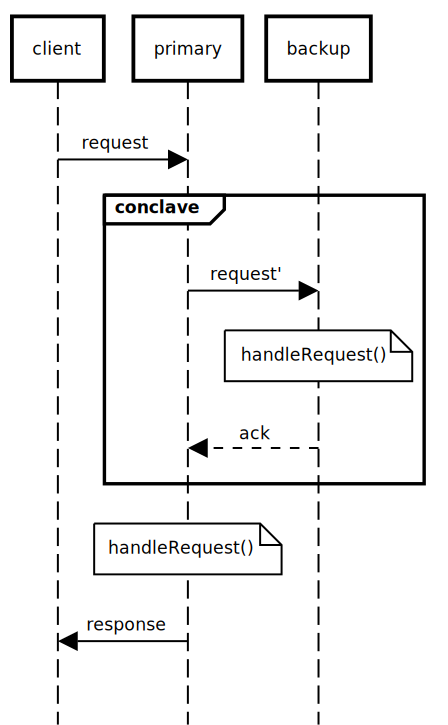
\includegraphics[width=4cm]{figures/seq3.pdf}
  \end{minipage} \\\\
  \multicolumn{2}{c}{\begin{minipage}{0.95\linewidth}
	  \textbf{(b)} In this variation, the \inlinecode{conclave} operator eliminates the redundant communication.
           The conclaved sub-choreography is indicated by a box in the sequence diagram.
           On line~3, \inlinecode{@@ nobody} is \MultiChor idiom explained in \Cref{sec:membership}.
  \end{minipage}}
  \end{tabular}
  \caption{Real Choreographies: a key-value store writing using \MultiChor, two variations.}
  \label{fig:kvsconclave}
    %%\Description{In the top section, twenty four lines of Haskell code using the MultiChor library, with a UML sequence diagram of that program.
%%	The code defines a choreography called "kvs", and helper-functions "handleRequest" and "handleBackup".
%%	In the sequence diagram, first "client" sends "request" to "server",
%%	  then "server" sends "request-prime" to "client" and "backup",
%%	  then backup calls "handleRequest",
%%	  then backup may send "ack" to "server",
%%	  then server calls "handleRequest",
%%	  then server sends "response" to "client.
%%	The bottom sections shows changes to the code in the top section.
%%	In particular, the return type of "handleBackup" is changed to exclude "client".
%%	In the updated sequence diagram, the part of the protocol representing "handleBackup" is in a box named "conclave",
%%	  and the spurious transmission of "request-prime" from "server" to "client" is omitted.
%%	  }
  \end{mdframed}
\end{figure}





\section{Background}
\label{sec:background}

Choreographic programming is a paradigm that expresses a distributed system
as a single, global program describing the behavior and interactions of all parties.
The global view of the distributed system enables easier reasoning about the system's behavior;
for example choreographic languages can ensure \emph{deadlock freedom}~\cite{montesi-carbone-dfbd}
and choreographies can be composed modularly like normal single-threaded protocols.

\subsection{History and Adjacent Domains}
\label{sec:history}

Theoretical and pragmatic frameworks for thinking clearly about concurrent and communicating systems are many and varied,
and include well known examples like Petri Nets that are over sixty years old~\cite{Petri1962}.
A number of other systems from the following decades are important both as historical markers and because modern research
builds directly on their ideas, their theory, structural patterns, and terminology.
The actor model~\cite{hewitt_actor_model} posits the description of an "actor" and their behavior as the fundamental
unit of a concurrent program, while being deliberately abstract about what an actor actually is.
Process- or \textpi-calculi are generally characterized by a designated syntax for parallelism
(actions that may happen in any order or simultaneously),
and typically have names or addresses associated with the participating processes and/or channels of communication between processes.
\cite{baeten2004} gives a good history of the field as it developed and diversified through the end of the 20\textsuperscript{th} century.

A basic goal in computer science is to provide guarantees that a program \emph{can't} exbibit a behavior that has been deemed bad,
\eg run-time exceptions or deadlocking;
a common way to accomplish this is by applying a type checker to the program.
One successful system (or style of system) for typing concurrent protocols has been \emph{multiparty session types} (MPST)~\cite{honda-mpsts}.
MPST encode a protocol of (possible sequences of) communication in a \emph{global type} in the language of MPST.
Projection of a global type to a named party ("endpoint") in the type yields a \emph{local type}
that can be ascribed to (and enforced against) an implementation (\eg in a \textpi-calculus) of that process's behavior\footnote{
	As in CP, the endpoint projection function in MPST is incomplete.
}.
In addition to the simple "what kind of thing might \inlinecode{x} be" sense of type safety,
MPST also provided communication safety (\eg a party never binds a received message to the wrong variable at runtime)
and a form of deadlock freedom.

Research extending MPST's expressiveness (the space of desirable programs that can be judged well-formed)
and safety (the space of undesired programs that can be statically rejected) is ongoing.
For example \cite{stutz2025} describe Automata-based Multiparty Protocols,
a MPST-like framework that, with various caveats, is more expressive than MPST and in which endpoint projection is total.
\cite{leBrun2025}, presented at the same conference, directly extend the syntax and semantics of MPST
with first-class process names and open-ended receiving channels;
in addition to the utility of these features \textit{per se}, this lets their system model mutual-exclusion and race conditions.
One way to think about choreographic programming is as the extension of the core ideas of MPST to include
\emph{both} the communication plan and the implementation of the computations each party is doing.

Although in this present work we use the noun "choreography" to refer to actual programs written in CP systems,
the word was already in use before the invention of choreographic programming \textit{per se}.
The broader sense of the word is any unified 3rd-person description of or plan for interaction between two or more participating systems.
Pseudo-code diagrams featuring a unified communication operator "→"
were being used to describe cryptographic protocols at least as early as 1978 \cite{needham_schroeder_1978}.
As an example,
\cite{w3c2005} presented the \emph{"Web Services Choreography Description Language"}
in which a user could specify the interaction, the sequence of communications, between parties.
Like MPST (introduced a few years later),
this was a specification language; implementations compatible with a given specification needed to be written separately.

Another technique for multiparty programming
(broadly, any technique for representing the behavior of a system of concurrent participants in as a single program)
is \emph{multitier programming}.
A multitier program has a "first person" perspective that privileges one party or role;
this perspective shifts to other roles, with implicit or explicit communication mediating these shifts.
ScalaLoci is an example of a multitier language with an embedded implementation in Scala and a formalism demonstrating its soundness~\cite{scalaLoci}.
A similar computational model named "first person choreographies", implemented as a Rascal proof-of-concept named 1CPLT,
omits ScalaLoci's reactive programming aspects~\cite{jongmans1cp2025}.
Of particular interest to our current work, both these languages can represent applications with variable quantities of participants.
The network behavior of a system built in these languages is less straightforward than that of a similar-looking choreography in two ways:
critical contextual information (roughly corresponding to Knowledge of Choice) is communicated implicitly,
and the exact communications that must or could happen (which depend on the variable quantities of participants) are determined dynamically.
Nonetheless, \cite{multiparty-languages} were able to show a degree of equivalence between minimalist models of multitier and choreographic programming.

\subsection{Endpoint Projection}
\label{sec:endpoint-projection}
CP systems necessarily include a means by which a given computer can execute the behavior of a role in the choreography.
Typically, this takes the form of a function from choreographies to programs in a "local" language
which the target computer can execute.
Such a function is parameterized by the target role, and is called \emph{Endpoint Projection} (EPP);
the roles are "endpoints", \ie surfaces from which and into which messages pass,
and the choreography is "projected" in the sense that the given endpoint's view of it is extracted.

As an example, EPP of the choreography in \Cref{fig:kvsconclave}\emph{(b)} to each of the three participants
would yield respective programs very similar to the ones in \Cref{fig:kvspiecewise},
except that the primary server would always send the request to the backup server
(and therefor the backup server would know how to proceed).

In a choreographic program, many (in some systems, all) values will be \emph{located}:
they will have explicit or implicit metadata indicating their owner.
EPP of a located value to its owner results in the value itself
(typically with the ownership annotation removed),
and EPP to anyone else results in a special placeholder symbol, \eg $\bot$.
The appearance of $\bot$ in a party's projection is not an error,
but attempting to do any semantic evaluation on $\bot$ would be,
so an important correctness property for choreographies is that parties never do that.

\subsection{Knowledge of Choice}
\label{sec:knowledge-of-choice}

Choreographies with conditionals
(\inlinecode{if}-expressions or anything that could be used for conditional control-flow)
introduce
a challenge for endpoint projection:
\emph{some parties might not know which branch to take!}
This challenge is referred to as the \emph{knowledge of choice}  (KoC)~\cite{castagna-knowledge-of-choice} problem.
All choreographic programming languages include a strategy for KoC
that ensures that relevant parties have enough information to play their part in the program.

The pseudo-code in \Cref{fig:kvspseudo} shows a simple instance of this exact problem:
\inlinecode{backup} doesn't know whether to expect a message or not,
because that decision depends on a value (\inlinecode{request'}) that \inlinecode{backup} doesn't have.
\Cref{fig:kvsconclave}\emph{(a)} implements the KoC strategy used by HasChor~\cite{shen-haschor}: the branch guard is broadcast to everyone.
HasChor's authors knew this to be an inefficient (but expedient) solution.
As we show in \Cref{fig:kvsconclave}\emph{(b)}, \MultiChor can do better.

A more traditional approach,
which we refer to as \emph{select-\&-merge},
is to include in one's language a special operator just for communicating KoC.
This operator is called "\inlinecode[bash]{select}"; it sends a statically-declared flag
to the recipient to select which of that party's possible behaviors should be activated.
For example, \Cref{fig:kvs_snm} shows how our KVS choreography might be expressed in a select-\&-merge system.
Under both the centralized semantics and type analysis, \inlinecode[bash]{select} is a no-op!
During EPP, \inlinecode[bash]{select} results in "offer" and "choose" actions at the receiver and sender, respectively.
Because \inlinecode[bash]{select} doesn't affect typing,
in \Cref{fig:kvs_snm} it would not be possible to encode the need for the lines~9 and~12 in Haskell's type system.
Instead, such CP systems enforce KoC requirements in their "merge" operator, which is applied during EPP.
Any party besides the owner of a branch guard will replace the entire conditional expression with the merge of their projections of the branches.
The merge of two "offer" expressions is an offer of the union of the possible continuations;
merges of any other combinations of expressions are only defined when the two expressions are the same.
Thus, if lines~9 and~12 were omitted from \Cref{fig:kvs_snm}, the error would be detected during EPP to \inlinecode{backup}
when the system tried to merge \inlinecode{{}} with
\begin{minted}[xleftmargin=30pt,fontsize=\small]{haskell}
{ request'' <- recv primary;
  success <- handleRequest request'' backupStateRef;
  send success primary  }
\end{minted}
A substantial body of research has explored the soundness select-\&-merge
and its fundamentals, implementation, and extensions
\cite{montesi-carbone-dfbd,core_choreographies,giallorenzo-choral,robust_choreographies}.
That said, HasChor, \MultiChor, ChoRus, and ChoreoTS all do EPP at runtime\cite{batesenclaves},
so using EPP to detect KoC problems would not be a satisfactory solution for them.

\begin{figure}[tbhp]
  \begin{mdframed}
  \begin{tabular}{c}
  \begin{minipage}{0.95\linewidth}
    \inputminted[xleftmargin=10pt,linenos,fontsize=\footnotesize]{haskell}{figures/kvs_snm.hs.txt}
  \end{minipage} \\\\
  \begin{minipage}{0.95\linewidth}
	  This pseudo-code choreography implements the protocol from \Cref{fig:kvsconclave}\emph{(b)}
	  using "select-\&-merge" syntax.
	  Attempting to engineer a real select-\&-merge CP eDSL in the style of \MultiChor
	  would result in a system that could not detect KoC errors until runtime.
  \end{minipage}
  \end{tabular}
  \caption{A Select-\&-Merge Choreography: a key-value store with a backup server}
  \label{fig:kvs_snm}
  \end{mdframed}
\end{figure}

Yet another KoC strategy was proposed by \cite{jongmans2022predicates}.
Their approach requires writing distinct guards for every
participant in a conditional expression; they show how to use predicate transformers to check that
such distributed decisions are unanimous.
This system is verbose, but at least as expressive as the one we describe in this work.

\subsection{The "Census" typing context}
\label{sec:census}
Although it is a hallmark of CP that a user may write actions for various parties in any given place in the program
without demarcations of who "control" is passing to,
it is not necessarily the case that every party that exists is eligible to take action at every place in the choreography.
Some earlier works, \eg \cite{chor-lambda}, have tracked these sets of participants in their type systems,
and used that typing context to control participation inside of function bodies.
Such a typing context plays a more active role in this present work, so we coin the term \emph{"census"}
for a typing context that controls which parties are "present" to participate in any given part of a choreography.
A party not listed in a census typically should not evaluate that section of the choreography;
exactly how that's enforced or implemented will depend on the system in question.

\subsection{Additional Literature}
\label{sec:modern-work}

Research and development of CP systems seems to have accelerated since approximately 2022.
Pirouette~\cite{hirsch2021pirouette}, Chorλ~\cite{chor-lambda},
and  PolyChorλ~\cite{graversen2023polychor}
are (higher order) functional languages for writing select-\&-merge choreographies;
PolChorλ additionally introduces polymorphism over identities of parties.
Choral~\cite{giallorenzo-choral} is a choreographic language implementing the select-\&-merge paradigm
and targeting industrial use;
it runs on the JVM and can easily import local Java code.
Dyno~\cite{zakhour23} is a CP system for Android development;
it's key feature is the ability to resolve the location and ownership of data and computation dynamically,
while still providing static safety guarantees.

Excitingly, CP libraries for a variety of general purpose languages have recently appeared on the scene.
These include UniChorn~\cite{unichorn}, Chorex~\cite{chorex-github}, and Klor~\cite{klor-github}.
All three are under development; here we report on their state toward the end of 2024.
UniChorn is a port of HasChor into the Unison programming language.
To implement EPP, it uses the Unison feature of \emph{abilities}, better known in the literature as algebraic effects~\cite{plotkin-2003,plotkin-2013}.
This implementation approach, which was also recently proposed by~\cite{shen-alg-eff-cp},
can be thought of as a generalization of the free(r)-monad approach.
As a direct port of HasChor, UniChorn does not support conclaves, MLVs, or census polymorphism.
Chorex is a CP system for Elixir, and Klor is a CP system for Clojure;
both Chorex and Klor leverage the powerful macro systems of their respective host languages to carry out EPP.
Chorex uses the select-\&-merge KoC strategy, and unprojectable choreographies can be detected at macro expansion time.
Klor, on the other hand, is effectively an conclaves-\&-MLVs system, but their API differs from the implementations we present here,
and the authors have not yet shown what safety guarantees it does or does not offer.
Neither Chorex nor Klor support census polymorphism.

Wysteria~\cite{wysteria} and Symphony~\cite{Sweet_2023} are domain-specific languages for \emph{secure multiparty computation}.
Programs in these languages can exhibit census polymorphism,
but they have homomorphic encryption baked into their
semantics for communication,
and they are not intended for general-purpose choreographic programming.
Wysteria has a \inlinecode{par} language construct, used for evaluating an expression at a set of locations,
that is somewhat similar in spirit to our conclaves.
However, applying the conclave concept to choreographic programming, and to the choreographic knowledge-of-choice problem in particular,
is to our knowledge a novel contribution of this paper.
Symphony does not support conditionals, and therefore KoC propagation is a moot point for them.

Another possible antecedent to census polymorphism as described in \Cref{sec:census-poly} is \cite{cp_practice_cruz_filipe_montesi},
which extends the syntax of Procedural Choreographies (PC) \cite{cp_procedural_cruz_filipe_montesi}
to support lists of processes as arguments to procedure calls.
Exact comparison between the extended PC system and \MultiChor is difficult for a few reasons:
First, PC is an advanced select-\&-merge system which tracks mutable network topology instead of a census.
Second, in PC's computational model processes serve double-duty as "participants" who do things and as "variables" that store data;
this is a sensible choice for their target usage context: parallelized object-oriented programming in which communication is cheap.
Understanding the limits of their syntax extensions in the context of their computational model is difficult because
the commensurate typing rule extensions not explicit.
Third, PC does not have an implementation.
We do not assert here whether either system's expressivity subsumes that of the other.


\bibliographystyle{chicago}
\bibliography{refs}

\chapter{A New Core Choreographic Calculus}
%\chaptermark{Formalism???} %this is the chapter heading that will show on subsequent pages
\label{sec:formalism}


\section{Introduction}
The HasChor library is inefficient in two ways.
The first is particular to its broadcast-based KoC strategy:
in order for any parities to branch on a value, the value must be broadcast to \emph{all} parties.
This can be overcome by adding censuses and \emph{conclaves} to the system.
The second shortcoming is shared in common with many select-\&-merge systems like Pirouette:
Sequential conditional clauses on the same branch-guard (\textit{aka} "scrutinee") require KoC to be \emph{re}communicated.
We address this issue by extending the notion of located values into \emph{multiply located values} (MLVs).
MLVs allow multiple parties to branch together on a shared guard;
in addition to recyclability, this alleviates the need for a designated \inlinecode[bash]{select} operator.
In this section we present \HLSCentral,
a formal model of a higher-order functional CP language that uses conclaves, census tracking, and MLVs
to guarantee proper KoC management entirely by type-checking and without compromising efficiency or expressivity.


\subsection{Multiply-located values}
\label{sec:mlvs}

Previous choreography languages have featured \emph{located values},
values annotated with (or implicitly assigned to) their owning party such that EPP to the owner results
in the value itself and EPP to any other party results in a special
"missing" value (\eg ⊥).
\emph{Multiply located values} are exactly the same except they are annotated with a non-empty \emph{set} of parties.
EPP of a multiply-located value for any of the owning parties results in the same value,
and projection to any other party yields ⊥.
Prior works have objects with multiple owners as emergent structures in a language
(\eg choreographic processes~\cite{giallorenzo-choral}, distributed choice types~\cite{chor-lambda-2}),
but these project to each owner's distinct view of the structure.

Creation of an MLV within an choreographic runtime follows from the fact that
if Alice sends Bob a number, both Alice and Bob know what number was sent.
Representing this in the language can be done a few different ways:
\begin{itemize}
  \item A \inlinecode{share} operator that updates the type of an MLV-typed variable to include the recipient(s) in the ownership set.
        This is a poor fit for a functional programming language because it mutates the type of a variable,
        and additional machinery would be needed to make it work with nested conclaves (see \Cref{sec:conclaves}).
  \item A \inlinecode{comm} operator that returns a value owned by the original owners and the recipient(s).
        This is not as straightforward as it sounds; if the communication happens inside a conditional,
        some of the original owners may not know that the communication happened.
        Intersecting with the current census is a sound solution,
        but may be difficult to embed in the type system of existing host languages.
  \item A \inlinecode{multicast} operator (by whatever name) that returns a value owned by exactly the specified recipients.
        In practice, users will often list the sender (and possibly any subset of the original owners) among the recipients;
        an ideal implementation would omit the actual communication to recipients who already have the data.
  \item A \inlinecode{broadcast} operator that always returns an MLV owned by the entire current census.
        This is actually equivalent to the above \inlinecode{multicast} operator; the choice is purely ergonomic.
\end{itemize}

Multiply-located values can also enable concise expression of programs in which multiple parties compute the same thing in parallel,
a common occurrence when communication is more expensive than computation.
For example, the \HLSCentral expression $5@\set{p,q,r}+3@\set{p,q,r}$ represents an addition performed in parallel by $p$, $q$, and $r$.

\subsection{Managing KoC with Conclaves and MLVs}
\label{sec:conclaves}

As discussed in \Cref{sec:census}, prior systems have tracked censuses as attributes of choreographic functions.
It's not usually required that every member of a census actually do anything in the choreography in question,
so (intuitively) if a choreography has some given census $\mathbf{C}$,
then it should be possible to embed that choreography inside a larger one with census $\mathbf{D}$,
provided $\mathbf{C}\subseteq\mathbf{D}$.
We call such sub-choreographies with sub-censuses \emph{conclaves}.
Any system with censuses likely has some version of conclaves,
but in prior systems like \chorLambda they were implicit side-effects of function application;
they did not affect the KoC strategy~\cite{chor-lambda}.
The ChoRus system introduced a designated conclave operator to explicitly limit the census within its argument,
and showed how this could be used to avoid HasChor's overly broad \inlinecode{broadcasts}\footnote{
	As discussed in \cite{batesenclaves}, ChoRus has since been upgraded to incorporate
	the innovations discussed in this work.
	\cite{chorus} is an unpublished pre-print describing their system as it existed without MLVs or census polymorphism.
  It uses the now-deprecated term \emph{"enclave"} instead of \emph{"conclave"}.
}.
An \inlinecode{conclave} operator is a good design choice for an embedded DSL,
but is not necessary in an abstract or bespoke language where the action of conclaving can be built into relevant constructs like
functions and conditionals.

The combination of censuses with conclaving and MLVs constitutes a novel KoC strategy,
on par with state-of-the-art select-\&-merge systems like \chorLambda in terms of communication efficiency
and more amenable to implementation as an eDSL.
The specific strategy is to require conditionals (control-flow branches) to conclave to the owners of their guard value.
This can be accomplished by broadcasting inside the conclave, or by passing in a MLV as the guard.
The advantage of using MLVs (aside from generally making things more concise)
is that they let conclaves return shared knowledge to for reuse in later conditionals.


\section{A Formal Conclaves-\&-MLVs Language}\label{sec:more-formalism}

We present the \HLSCentral CP system.
The syntax of \HLSCentral and our overarching computational model and proof-approach are loosely based on
Chorλ~\cite{chor-lambda}.
\HLSCentral is a higher-order choreographic lambda calculus;
we omit recursion and polymorphism because they are orthogonal to our goals here.
Specifically, we will show that multiply-located values and conclaving operations are sufficient for a sound
CP language without further KoC management.
In \Crefrange{sec:syntax}{sec:semantics}
we describe the syntax, type system, and semantics of \HLSCentral.
As in other choreographic languages, the primary semantics describes the intended \emph{meaning} of choreographies
and can be used to reason about their behavior,
but is not the "ground truth" of concurrent execution.
\Crefrange{sec:local-lang}{sec:networks} describe the languages of distributed processes,
\HLSLocal and \HLSNet,
and define endpoint projection for \HLSCentral.
%
In \Cref{sec:deadlock-freedom}, we prove that the behavior of a choreography's projection in \HLSNet
matches that of the original \HLSCentral choreography, and that \HLSCentral's type system ensures deadlock-freedom.
In \Cref{sec:formalism-comparisons} we provide some example choreographies in (a plain-text rendering of) \HLSCentral.
For example, \Cref{fig:our-kvs} implements the KVS example from \Cref{sec:introduction}.

\subsection{Syntax}\label{sec:syntax}
The syntax of \HLSCentral is in \Cref{fig:syntax}.
Location information sufficient for typing, semantics, and EPP is explicit in
the expression forms.
We distinguish between "pairs"
($\PAIR V_1 V_2$, of type $(d_1 × d_2)@\nonempty{p}$)
and "tuples"
($(V_1, V_2)$, of type $(T_1, T_2)$)
so that we can have a distinguishable concept of "data" as "stuff that can be sent";
we do not believe this to have any theoretic significance.

The superscript-marked identifier $\nonempty{p}$ is a semantic token representing a set of parties;
an unmarked $p$ is a completely distinct token representing a single party.
Note the use of a superscript "$+$" to denote sets of parties
instead of a hat or boldface;
this denotes that these lists may never be empty.\footnote{
Later, we'll use an "$\ast$" to denote a possibly-empty set or list,
and a "$?$" to denote "zero or one".
}
The typing and semantic rules will enforce this invariant as needed.
When referring to a census, or when a set of parties should be understood as a "context"
rather than an "attribute",
we write Θ rather than $\nonempty{p}$;
this is entirely to clarify intent and the distinction has no formal meaning.

\begin{figure}[tbhp]
\footnotesize
    \begin{mdframed}
\begin{align*}
M  \BNF   &  V                       && \text{Values.}          \\
   \BNFOR &  M M                     && \text{Function application.}          \\
   \BNFOR &  \CASE{\nonempty{p}}{M}{x}{M}{x}{M}    \quad&& \text{Branching on a disjoint-sum value.}          \\
                                            \\
V  \BNF   &  x                       && \text{Variables.}          \\
   \BNFOR &  (λ x:T \DOT M)@\nonempty{p}            && \text{Function literals annotated with participants.}          \\
   \BNFOR &  ()@\nonempty{p}                      && \text{Multiply-located unit.}          \\
   \BNFOR &  \INL V                  && \text{Injection to a disjoint-sum.}           \\
   \BNFOR &  \INR V                  && \text{}           \\
    \BNFOR &  \PAIR V V               && \text{Construction of data pairs (products).}           \\
   \BNFOR &  (V, \dots, V)           && \text{Construction of heterogeneous tuples.}           \\
   \BNFOR &  \FST{\nonempty{p}}      && \text{Projection of data pairs.}           \\
   \BNFOR &  \SND{\nonempty{p}}      && \text{}           \\
   \BNFOR &  \LOOKUP{n}{\nonempty{p}}   && \text{Projection of tuples.}           \\
   \BNFOR &  \COMM{p}{\nonempty{p}}     && \text{Send to one or more recipients.}            \\
                                            \\
d  \BNF   &  ()         && \text{We provide a simple algebra of "data" types,}   \\
   \BNFOR &  d + d                   && \text{which can encode booleans or other finite types}           \\
   \BNFOR &  d × d                   && \text{and could be extended with natural numbers if desired.}   \\
                                            \\
T  \BNF   &  d@\nonempty{p}          && \text{A complete multiply-located data type.}             \\
    \BNFOR &  (T → T)@\nonempty{p}          && \text{Functions are located at their participants.}             \\
   \BNFOR &  (T, \dots, T)           && \text{A fixed-length heterogeneous tuple.}  \\
\end{align*}
    \caption{The complete syntax of the \HLSCentral language.}
    \label{fig:syntax}
    %\Description[A BNF syntax for a choreographic lambda calculus.]
     %           {A BNF syntax for a choreographic lambda calculus.
      %          There are three expression-forms M,
       %         including the V form for values,
        %        of which there are eleven sub-forms.
         %       There are also forms for types.
          %      Both types and expressions have party-annotations.}
    \end{mdframed}
\end{figure}

\subsection{The Mask Operator}\label{sec:masking}
Here we introduce the \mask operator,
the purpose of which is to allow \Cref{theorem:preservation}
(semantic stepping preserves types)
to hold
without adding sub-typing or polymorphism to \HLSCentral.
\mask is a partial function defined in \Cref{fig:masking};
the left-hand argument is either a type (in which case it returns a type)
or a value (in which case it returns a value).
The effect of \mask is very similar to EPP,
except that it projects to a set of parties instead of just one,
and instead of introducing a ⊥ symbol it is simply undefined in some cases.
Because it is used during type-checking, errors related to it are caught at that time.

Consider an expression using a "masking identity" function:
$(λ x:()@\set{p} \DOT x)@\set{p} ()@\set{p,q}$,
where the lambda is an identity function \emph{application of which}
turns a multiply-located unit value into one located at just $p$.
Clearly, the lambda should type as $(()@\set{p} → ()@\set{p})@\set{p}$;
and so the whole application expression should type as $()@\set{p}$.
Masking in the typing rules lets this work as expected,
and similar masking in the semantic rules ensures type preservation.

\begin{figure}[tbhp]
\footnotesize
    \begin{mdframed}
\begin{gather*}
\myference{MTData}
          {\nonempty{p} ∩ Θ ≠ ∅}
          {d@\nonempty{p} \mask Θ \DEF d@(\nonempty{p} ∩ Θ)}
          \quad
\myference{MTFunction}
          {\nonempty{p} \subseteq Θ}
          {(T → T')@\nonempty{p} \mask Θ \DEF (T → T')@\nonempty{p}}
          \vdbl
\myference{MTVector}
          {T_1' = T_1 \mask Θ, \quad \dots \quad T_n' = T_n \mask Θ}
          {(T_1, \dots, T_n) \mask Θ \DEF (T_1', \dots, T_n')}
          \vdbl
\myference{MVLambda}
          {\nonempty{p} \subseteq Θ}
          {(λ x:T \DOT M)@\nonempty{p} \mask Θ \DEF (λ x:T \DOT M)@\nonempty{p}}
          \quad
\myference{MVUnit}
          {\nonempty{p} ∩ Θ ≠ ∅}
          {()@\nonempty{p} \mask Θ \DEF ()@(\nonempty{p} ∩ Θ)}
          \vdbl
\myference{MVInL}
          {V' = V \mask Θ}
          {\INL V \mask Θ \DEF \INL V'}
          \quad
\myference{MVInR}
          {\dots}
          {\dots}
          \quad
\myference{MVProj1}
          {\nonempty{p} \subseteq Θ}
          {\FST{\nonempty{p}} \mask Θ \DEF \FST{\nonempty{p}}}
          \quad
\myference{MVProj2}
          {\dots}
          {\dots}
          \vdbl
\myference{MVPair}
          {V_1' = V_1 \mask Θ \quad V_2' = V_2 \mask Θ}
          {\PAIR V_1 V_2 \mask Θ \DEF \PAIR V_1' V_2'}
          \quad
\myference{MVVector}
          {V_1' = V_1 \mask Θ \quad \dots \quad V_n' = V_n \mask Θ}
          {(V_1, \dots, V_n) \mask Θ \DEF (V_1', \dots, V_n')}
          \vdbl
\myference{MVProjN}
          {\nonempty{p} \subseteq Θ}
          {\LOOKUP{n}{\nonempty{p}} \mask Θ \DEF \LOOKUP{n}{\nonempty{p}}}
          \quad
\myference{MVCom}
          {s \in Θ \quad \nonempty{r} \subseteq Θ}
          {\COMM{s}{\nonempty{r}} \mask Θ \DEF \COMM{s}{\nonempty{r}}}
          \quad
\myference{MVVar}
          {}
          {x \mask Θ \DEF x}
\end{gather*}
    \caption{Definition of the \mask operator.}
    \label{fig:masking}
%    \Description[Inference rules defining a partial function "mask".]
 %               {Inference rules defining a partial function "mask"
  %              denoted by a rightward triangle.
   %             The right-hand argument is a non-empty set of parties,
    %            and the left-hand argument is either a type or a value.
     %           It's defined as the left-hand argument re-located
      %          to the right-hand argument, provided the new locations
       %         are a subset of the original locations and that the new value
        %        is still semantically useable.}
    \end{mdframed}
\end{figure}

\subsection{Typing Rules}\label{sec:typing}
The typing rules for \HLSCentral are in \Cref{fig:typing}.
A judgment $Θ;Γ ⊢ M : T$ says that $M$ has type $T$ in the context
of a non-empty census Θ
and a (possibly empty) list of variable bindings $Γ=(x_1:T_1), \dots (x_n:T_n)$.
In \textsc{TLambda} and \textsc{TProjN} we write preconditions
$\noop{\nonempty{p}}{T}$ meaning $T = T \mask \nonempty{p}$,
\ie masking to those parties is a "no-op".

\begin{figure}[tbhp]
\footnotesize
    \begin{mdframed}
\begin{gather*}
\myference{TLambda}
          {\nonempty{p};Γ,(x:T) ⊢ M : T' \quad
           \nonempty{p} \subseteq Θ \quad
           \noop{\nonempty{p}}{T}}
          {Θ;Γ ⊢ (λ x:T \DOT M)@\nonempty{p} : (T → T')@\nonempty{p}}
          \quad
\myference{TVar}
          {x : T \in Γ \quad T' = T \mask Θ}
          {Θ;Γ ⊢ x : T' }
          \vdbl
\myference{TApp}
          {Θ;Γ ⊢ M : (T_a → T_r)@\nonempty{p} \quad
           Θ;Γ ⊢ N : T_a' \quad
           T_a' \mask \nonempty{p} = T_a}
          {Θ;Γ ⊢ M N : T_r}
          \vdbl
\myference{TCase}
          {Θ;Γ ⊢ N : T_N \quad
           (d_l + d_r)@\nonempty{p} = T_N \mask \nonempty{p} \\
           \nonempty{p};Γ,(x_l:d_l@\nonempty{p}) ⊢ M_l : T \quad
           \nonempty{p};Γ,(x_r:d_r@\nonempty{p}) ⊢ M_r : T \quad
           \nonempty{p} \subseteq Θ}
          {Θ;Γ ⊢ \CASE{\nonempty{p}}{N}{x_l}{M_l}{x_r}{M_r} : T}
          \vdbl
\myference{TUnit}
          {\nonempty{p} \subseteq Θ}
          {Θ;Γ ⊢ ()@\nonempty{p} : ()@\nonempty{p}}
          \quad
\myference{TPair}
          {Θ;Γ ⊢ V_1 : d_1@\nonempty{p_1} \quad
           Θ;Γ ⊢ V_2 : d_2@\nonempty{p_2} \quad
           \nonempty{p_1} ∩ \nonempty{p_2} ≠ ∅}
          {Θ;Γ ⊢ \PAIR V_1 V_2 : (d_1 × d_2)@(\nonempty{p_1} ∩ \nonempty{p_2})}
          \vdbl
\myference{TVec}
          {Θ;Γ ⊢ V_1 : T_1 \quad \dots \quad Θ;Γ ⊢ V_n : T_n}
          {Θ;Γ ⊢ (V_1, \dots, V_n) : (T_1, \dots T_n)}
          \quad
\myference{TInl}
          {Θ;Γ ⊢ V : d@\nonempty{p}}
          {Θ;Γ ⊢ \INL V : (d + d')@\nonempty{p}}
          \quad
\myference{TInr}{\dots}{\dots}
          \vdbl
\myference{TProjN}
          {\nonempty{p} \subseteq Θ \quad
           \noop{\nonempty{p}}{(T_1, \dots, T_n)}}
          {Θ;Γ ⊢ \LOOKUP{i}{\nonempty{p}} : ((T_1, \dots, T_i, \dots, T_n) → T_i)@\nonempty{p}}
          \quad
\myference{TProj2}{\dots}{\dots}
          \vdbl
\myference{TProj1}
          {\nonempty{p} \subseteq Θ}
          {Θ;Γ ⊢ \FST{\nonempty{p}} : ((d_1 × d_2)@\nonempty{p} → d_1@\nonempty{p})@\nonempty{p}}
          \vdbl
\myference{TCom}
          {s \in \nonempty{s} \quad
           \nonempty{s}\cup\nonempty{r} \subseteq Θ}
          {Θ;Γ ⊢ \COMM{s}{\nonempty{r}} : (d@\nonempty{s} → d@\nonempty{r})@(\set{s}\cup\nonempty{r})}
\end{gather*}
    \caption{\HLSCentral typing rules.}
    \label{fig:typing}
    %\Description[Inference rules for he-lambda-small's type system.]
     %           {Inference rules for he-lambda-small's type system.
      %          There are thirteen of them, corresponding to the thirteen
       %         total expression forms.}
    \end{mdframed}
\end{figure}

Examine \textsc{TCase} as the most involved example.
The actual judgment says that in the context of Θ and Γ,
the case expression types as $T$.
The first two preconditions say that
the guard expression $N$ must type in the parent context
as some type $T_N$, which masks to the explicit party-set $\nonempty{p}$
as a sum-type $(d_l + d_r)@\nonempty{p}$.
The only rule by which it can do that is \textsc{MTData},
so we can deduce that $T_N = (d_l + d_r)@\nonempty{q}$,
where $\nonempty{q}$ is some unspecified superset of $\nonempty{p}$.
The third and forth preconditions require the bodies of the expression to conclave correctly: $M_l$ and $M_r$
must both type as $T$ with the reduced census $\nonempty{p}$
(and with the respective $x_l$ and $x_r$ bound to the right and left
data types at $\nonempty{p}$).
The final precondition says that $\nonempty{p}$ is a subset of Θ,
\ie everyone who's supposed to be branching is actually present to do so.

The other rules are mostly normal, with similar masking of types and conclaving of censuses as needed.
In \textsc{TVar}, the census masks the type bindings in Γ.
In isolation, some expressions such as $\INR ()@\set{p}$
or the projection operators
are flexible about their exact types;
additional annotations could give them monomorphic typing,
if that was desirable.

\subsection{Masked Substitution}\label{sec:substitution}

For \mask to fulfil its purpose during semantic evaluation,
it may need to be applied arbitrarily many times with different party-sets
inside the new expressions, and it may not even be defined for all such
party-sets.
Conceptually, this just recapitulates the masking performed in \textsc{TVar}.
To formalize these subtleties, in \Cref{fig:substitution} we specialize the normal variable-substitution
notation $M[x:=V]$ to perform location-aware substitution.
In \Cref{sec:substitution-proof} we prove \Cref{theorem:substitution},
which shows that this specialized substitution operation
satisfies the usual concept of substitution.
(Our various definitons and proofs about them in this work all assume Barendregt’s variable convention.
Roughly, this says that bound variables are unique.
\cite{barendregtDiscussion} provide a more detailed discussion.)
\begin{theorem}[Substitution]\label{theorem:substitution}
  If $Θ;Γ,(x:T_x) ⊢ M : T$ and $Θ;Γ ⊢ V : T_x$,
  then $Θ;Γ ⊢ M[x := V] : T$.
\end{theorem}

\begin{figure}[tbhp]
\footnotesize
    \begin{mdframed}
\begin{align*}
M[x:=V] \DEF \text{by pattern matching on $M$:}& \\
y            \DEFCASE & \begin{cases}
                                        y ≡ x & \DEFCASE  V  \\
                                        y ≢ x & \DEFCASE  y
                                        \end {cases} \\
N_1 N_2     \DEFCASE & N_1[x:=V] N_2[x:=V] \\
(λ y:T \DOT N)@\nonempty{p}  \DEFCASE & \begin{cases}
                                        V \mask \nonempty{p} = V'
                                            & \DEFCASE (λ y:T \DOT N[x:=V'])@\nonempty{p} \\
                                        \text{otherwise} & \DEFCASE M
                                        \end{cases} \\
\CASEm{\nonempty{p}}{N}{x_l}{M_l}{x_r}{M_r} \DEFCASE & \begin{cases}
                                        V \mask \nonempty{p} = V'
                                            & \DEFCASE \CASEm{\nonempty{p}}
                                                            {N[x:=V]}{x_l}{M_l[x:=V']}
                                                            {x_r}{M_r[x:=V']} \\
                                        \text{otherwise}
                                            & \DEFCASE \CASEm{\nonempty{p}}
                                                            {N[x:=V]}{x_l}{M_l}{x_r}{M_r}
                                        \end{cases} \\
\INL V_1    \DEFCASE & \INL V_1[x:=V] \\
\INR V_2    \DEFCASE & \INR V_2[x:=V] \\
\PAIR V_1 V_2  \DEFCASE & \PAIR V_1[x:=V] V_2[x:=V] \\
(V_1, \dots, V_n) \DEFCASE & (V_1[x:=V], \dots, V_n[x:=V]) \\
\begin{rcases}
    ()@\nonempty{p}
    \qquad \FST{\nonempty{p}}
    \qquad \SND{\nonempty{p}} \\
    \qquad \LOOKUP{\nonempty{p}}{i}
    \qquad \COMM{s}{\nonempty{r}}
\end{rcases}\DEFCASE & M
\end{align*}
    \caption{The customised substitution used in \HLSCentral's semantics.}
    \label{fig:substitution}
    %\Description[A case-wise definition of variable substitution.]
     %           {A case-wise definition of variable substitution.
      %           Most cases are normal; some involve masking
       %          and when the masking is undefined they revert to a no-op.}
    \end{mdframed}
\end{figure}


\subsection{Centralized Semantics}\label{sec:semantics}

The semantic stepping rules for evaluating \HLSCentral expressions
are in \Cref{fig:semantics}.
In \Cref{sec:local-lang,sec:projection,sec:networks}
we will develop the "ground truth" of the distributed process semantics and show that
the \HLSCentral's semantics correctly capture distributed behavior.

\HLSCentral is equipped with a substitution-based semantics that,
after accounting for the \mask operator and the specialized implementation of
substitution, is quite standard among lambda-calculi.
In particular, we make no effort here to support the out-of-order execution
supported by some choreography languages.
Because the language and corresponding computational model are parsimonious,
no step-annotations are needed for the centralized semantics.

\begin{figure}[tbhp]
    \begin{mdframed}
\begin{gather*}
\myference{AppAbs}
          {V' = V \mask \nonempty{p}}
          {((λ x:T \DOT M)@\nonempty{p}) V \step M[x := V']}
          \quad
\myference{App1}
          {N \step N'}
          {V N \step V N'}
          \quad
\myference{App2}
          {M \step M'}
          {M N \step M' N}
          \vdbl
\myference{Case}
          {N \step N'}
          {\CASE{\nonempty{p}}{N}{x_l}{M_l}{x_r}{M_r}
            \step \CASE{\nonempty{p}}{N'}{x_l}{M_l}{x_r}{M_r}}
          \vdbl
\myference{CaseL}
          {V' = V \mask \nonempty{p}}
          {\CASE{\nonempty{p}}{\INL V}{x_l}{M_l}{x_r}{M_r} \step M_l[x_l := V']}
          \quad
\myference{CaseR}
          {\dots}
          {\dots}
          \vdbl
\myference{Proj1}
          {V' = V_1 \mask \nonempty{p}}
          {\FST{\nonempty{p}} (\PAIR V_1 V_2) \step V'}
          \quad
\myference{Proj2}
          {\dots}
          {\dots}
          \quad
\myference{ProjN}
          {V' = V_i \mask \nonempty{p}}
          {\LOOKUP{i}{\nonempty{p}} (V_1, \dots, V_i, \dots, V_n) \step V'}
          \vdbl
\myference{Com1}
          {()@\nonempty{p} \mask \set{s} = ()@s}
          {\COMM{s}{\nonempty{r}} ()@\nonempty{p} \step ()@\nonempty{r}}
          \quad
\myference{ComPair}
          {\COMM{s}{\nonempty{r}} V_1 \step V_1' \quad \COMM{s}{\nonempty{r}} V_2 \step V_2'}
          {\COMM{s}{\nonempty{r}} (\PAIR V_1 V_2) \step \PAIR V_1' V_2'}
          \vdbl
\myference{ComInl}
          {\COMM{s}{\nonempty{r}} V \step V'}
          {\COMM{s}{\nonempty{r}} (\INL V) \step \INL V'}
          \quad
\myference{ComInr}
          {\dots}
          {\dots}
\end{gather*}
    \caption{\HLSCentral's semantics.}
    \label{fig:semantics}
%    \Description[Infernce rules for the central language.]
 %               {Thirteen inference rules defining the semantics of
  %               choreographies.
   %             Most of them are entirely normal lambda-calculus rules
    %            except that they use a mask operator and a specialized
     %           notion of substitution.
      %          The exceptions are the COM rules, which use each other
       %         as recursive preconditions to replace the location annotations
        %        on unit values.}
    \end{mdframed}
\end{figure}

The \textsc{Com1} rule simply replaces one location-annotation with another.
\textsc{ComPair}, \textsc{ComInl}, and \textsc{ComInr} are defined recursively
amongst each other and \textsc{Com1};
the effect of this is that "data" values can be sent but other values
(functions and variables) cannot.

As is typical for a typed lambda calculus, \HLSCentral enjoys preservation and progress.

\begin{theorem}[Preservation]\label{theorem:preservation}
  If $Θ;∅ ⊢ M : T$ and $M \step M'$, then $Θ;∅ ⊢ M' : T$.
\end{theorem}

\begin{theorem}[Progress]\label{theorem:progress}
  If $Θ;∅ ⊢ M : T$, then either M is of form $V$ (which cannot step)
  or their exists $M'$ s.t. $M \step M'$.
\end{theorem}

We prove these properties in \Cref{sec:preservation-proof,sec:progress-proof} respectively.


\subsection{The Local Process Language}\label{sec:local-lang}

In order to define EPP and a "ground truth" for \HLSCentral computation,
we need a locally-computable language, \HLSLocal, into which it can project.
\HLSLocal is very similar to \HLSCentral;
to avoid ambiguity we denote \HLSLocal expressions $B$ (for "behavior")
instead of $M$ (which denotes a \HLSCentral expression)
and \HLSLocal values $L$ instead of $V$.
The syntax is presented in \Cref{fig:local-syntax}.

\begin{figure}[tbhp]
    \begin{mdframed}
    \begin{align*}
        B \BNF   & L \BNFOR B B && \text{\small Process expressions.} \\
          \BNFOR & \CASE{}{B}{x}{B}{x}{B} \\[0.5em]
        L \BNF   & x \BNFOR () \BNFOR   λ x \DOT B
                     && \text{\small Process values.} \\
          \BNFOR & \INL L \BNFOR \INR L \BNFOR  \PAIR L L \\
          \BNFOR & \FST{} \BNFOR \SND{} \\
          \BNFOR & (L, \dots, L) \BNFOR \LOOKUP{n}{} && \text{} \\
          \BNFOR & \RECV{p} \BNFOR \SEND{p^{\ast}}
                     && \text{\small Receive from one party. Send to many.} \\
          \BNFOR & \SEND{p^{\ast}}^{\ast}
                    && \text{\small Send to many \emph{and} keep for oneself.} \\
          \BNFOR & ⊥                  && \text{\small "Missing" (located someplace else).}
    \end{align*}
    \caption{Syntax for the \HLSLocal language.}
    \label{fig:local-syntax}
    %\Description[A BNF for a simple lambda calculus with "send" and "receive" operators.]
     %           {A BNF for a simple lambda calculus with "send" and "receive" operators.
      %          By design, it's very similar to the central language, just without party annotations
       %         and with "com" replaced by "send", "send*", and "recv".}
    \end{mdframed}
\end{figure}

\HLSLocal differs from \HLSCentral in a few ways.
It's untyped, and the party-set annotations are mostly missing.
\HLSCentral's $\COMM{p}{\nonempty{q}}$ operator is replaced by $\SEND{\nonempty{q}}$ and $\RECV{p}$,
as well as a $\SEND{\nonempty{q}}^{\ast}$, which differs from $\SEND{\nonempty{q}}$ only in that
the process which calls it keeps a copy of the sent value for itself.
Syntactically, the recipient lists of $\SEND{}$ and $\SEND{}^{\ast}$ may be empty;
this keeps semantics consistent in the edge case implied by
a \HLSCentral expression like $\COMM{s}{\set{s}}$ (which is useless but legal).
Finally, the value-form ⊥ ("bottom") is a stand-in for parts of the choreography that do not involve the target party.
In the context of choreographic languages, ⊥ does not denote an error but should instead be read as "unknown"
or "somebody else's problem".

The behavior of ⊥ during semantic evaluation can be handled a few different ways,
the pros-and-cons of which are not important in this work.
We use a ⊥-normalizing "floor" function, defined in \Cref{fig:floor},
during EPP and semantic stepping to avoid ever handling
⊥-equivalent expressions like $\PAIR ⊥ ⊥$ or $⊥ ()$.

\begin{figure}[tbhp]
\footnotesize
    \begin{mdframed}
\begin{align*}
\FLR{B}                        \DEF      \text{by pattern matching on $B$:}
  & \qquad\qquad\qquad\qquad  \text{\small{(Observe that floor is idempotent.)}} \\
B_1 B_2                      \DEFCASE &
  \begin{cases}
    \FLR{B_1} = ⊥, \FLR{B_2} = L \DEFCASE & ⊥  \\
    \text{else}              \DEFCASE & \FLR{B_1} \FLR{B_2}
  \end{cases}  \\
\CASE{}{B_G}{x_l}{B_l}{x_r}{B_r} \DEFCASE &
  \begin{cases}
    \FLR{B_G} = ⊥                \DEFCASE & ⊥ \\
    \text{else}      \DEFCASE & \CASE{}{\FLR{B_G}}{x_l}{\FLR{B_l}}{x_r}{\FLR{B_r}}
  \end{cases}  \\
λ x \DOT B'                  \DEFCASE & λ x \DOT \FLR{B'} \\
\INL L                       \DEFCASE & \begin{cases}
  \FLR{L} = ⊥                \DEFCASE & ⊥ \\
  \text{else}                \DEFCASE & \INL \FLR{L}
  \end{cases} &&      \\
\INR L                       \DEFCASE & \begin{cases}
  \FLR{L} = ⊥                \DEFCASE & ⊥ \\
  \text{else}                \DEFCASE & \INR \FLR{L}
  \end{cases} &&      \\
\PAIR L_1 L_2                \DEFCASE & \begin{cases}
  \FLR{L_1} = ⊥ = \FLR{L_2}  \DEFCASE & ⊥ \\
  \text{else}                \DEFCASE & \PAIR \FLR{L_1} \FLR{L_2}
  \end{cases} &&         \\
(L_1, \dots, L_n)            \DEFCASE & \begin{cases}
  \forall_{i\in[1,n]} \FLR{L_i} = ⊥ \DEFCASE & ⊥ \\
  \text{else}                \DEFCASE & (\FLR{L_1}, \dots, \FLR{L_n})
  \end{cases} && \\
\begin{rcases}
  x \\
  () \\
  \FST{} \\
  \SND{} \\
  \LOOKUP{i}{} \\
  \SEND{p^{\ast}} \\
  \SEND{p^{\ast}}^{\ast} \\
  \RECV{p} \\
  ⊥
\end{rcases}                 \DEFCASE &  B
\end{align*}
    \caption{The "floor" function, which reduces ⊥-based expressions.}
    \label{fig:floor}
    %\Description[A casewise definition of a function using the bottom-brackets associated with a real-number "floor" function.]
     %           {A casewise definition of a function, using the bottom-brackets associated with a real-number "floor" function,
      %          that takes a local-language expression and returns it with "bottom" values simplified.}
    \end{mdframed}
\end{figure}


\HLSLocal's semantic stepping rules are given in \Cref{fig:local-semantics}.
Local steps are labeled with send ($⊕$) and receive ($⊖$) sets, like so:
$B \prcstep{\set{(p,L_1), (q,L_2)}}{\set{(r, L_3), (s, L_4)}} B'$,
or $B \prcstep{μ}{η} B'$ when we don't need to inspect the contents of the annotations.
The floor function is used to keep expressions normalized during evaluation.
Otherwise, most of the rules are analogous to the corresponding \HLSCentral rules from \Cref{fig:semantics}.
The \textsc{LSend-} rules are defined recursively, similar to the \textsc{Com-} rules.
\textsc{LSendSelf} shows that $\SEND{}^{\ast}$ is exactly like $\SEND{}$
except it locally acts like \inlinecode{id} instead of returning ⊥.
\textsc{LRecv} shows that the $\RECV{}$ operator ignores its argument and can return
\emph{anything}, with the only restriction being that the return value must be reflected in the receive-set step-annotation.

\begin{figure}[tbhp]
\footnotesize
    \begin{mdframed}
\begin{gather*}
\myference{LAbsApp}
          {}
          {(λ x \DOT B) L \prcstep{∅}{∅} \FLR{B[x:=L]}}
          \quad
\myference{LApp1}
          {B \prcstep{μ}{η} B'}
          {L B \prcstep{μ}{η} \FLR{L B'}}
          \quad
\myference{LApp2}
          {B \prcstep{μ}{η} B'}
          {B B_2 \prcstep{μ}{η} \FLR{B' B_2}}
          \vdbl
\myference{LCase}
          {B \prcstep{μ}{η} B'}
          {\CASE{}{B}{x_l}{B_l}{x_r}{B_r} \prcstep{μ}{η}
           \FLR{\CASE{}{B'}{x_l}{B_l}{x_r}{B_r}}}
          \vdbl
\myference{LCaseL}
          {}
          {\CASE{}{\INL L}{x_l}{B_l}{x_r}{B_r} \prcstep{∅}{∅} \FLR{B_l[x_l := L]}}
          \quad
\myference{LCaseR}
          {\dots}
          {\dots}
          \vdbl
\myference{LProj1}
          {}
          {\FST{} (\PAIR L_1 L_2) \prcstep{∅}{∅} L_1}
          \quad
\myference{LProj2}
          {\dots}
          {\dots}
          \quad
\myference{LProjN}
          {}
          {\LOOKUP{i}{} (L_1, \dots, L_i, \dots, L_n) \prcstep{∅}{∅} L_i}
          \vdbl
\myference{LSend1}
          {}
          {\SEND{p^{\ast}} () \prcstep{\set{(p, ()) \mid p \in p^{\ast}}}{∅} ⊥}
          \quad
\myference{LSendPair}
          {\SEND{p^{\ast}} L_1 \prcstep{μ_1}{∅} ⊥ \quad
           \SEND{p^{\ast}} L_2 \prcstep{μ_2}{∅} ⊥}
          {\SEND{p^{\ast}} (\PAIR L_1 L_2)
           \prcstep{\set{(p, \PAIR L_1 L_2) \mid p \in p^{\ast}}}{∅}
           ⊥}
          \vdbl
\myference{LSendInL}
          {\SEND{p^{\ast}} L \prcstep{μ}{∅} ⊥}
          {\SEND{p^{\ast}} (\INL L)
           \prcstep{\set{(p, \INL L) \mid p \in p^{\ast}}}{∅}
           ⊥}
          \quad
\myference{LSendInR}
          {\dots}
          {\dots}
          \quad
\myference{LSendSelf}
          {\SEND{p^{\ast}} L \prcstep{μ}{∅} ⊥}
          {\SEND{p^{\ast}}^\ast L \prcstep{μ}{∅} L}
          \vdbl
\myference{LRecv}
          {}
          {\RECV{p} L_0 \prcstep{∅}{\set{(p, L)}} L}
          \quad
\end{gather*}
    \caption{The semantics of \HLSLocal.}
    \label{fig:local-semantics}
    %\Description[Fifteen inference rules defining the semantics of the local process language.]
     %           {Inference rules defining the substitution-based semantic stepping of the local process language.
      %          There are fifteen rules, roughly corresponding to the similar rules from the choreographic semantics.}
    \end{mdframed}
\end{figure}

\subsection{Endpoint Projection}\label{sec:projection}
Endpoint projection (EPP) is the translation between the choreographic language \HLSCentral
and the local process language \HLSLocal;
necessarily it's parameterized by the specific
local process you're projecting \emph{to}.
$⟦M⟧_p$ is the projection of $M$ to $p$, as defined in \Cref{fig:eep}.
It does a few things:
Most location annotations are removed, some expressions become ⊥,
⊥-based expressions are normalized by the floor function,
and $\COMM{s}{\nonempty{r}}$ becomes $\SEND{\nonempty{r}}$, $\SEND{\nonempty{r}}^{\ast}$, or $\RECV{s}$,
keeping only the identities of the peer parties and not the local party.

\begin{figure}[tbhp]
\footnotesize
    \begin{mdframed}
\begin{align*}
⟦M⟧_p                        \DEF      \text{by pattern matching on $M$:}& \\
N_1 N_2                      \DEFCASE & \FLR{⟦N_1⟧_p ⟦N_2⟧_p} \\
\CASEm{\nonempty{p}}{N}{x_l}{M_l}{x_r}{M_r} \DEFCASE &
  \begin{cases}
    p \in \nonempty{p}       \DEFCASE & \FLR{
      \CASE{}{⟦N⟧_p}{x_l}{⟦M_l⟧_p}{x_r}{⟦M_r⟧_p} } \\
    \text{else}              \DEFCASE & \FLR{
      \CASE{}{⟦N⟧_p}{x_l}{⊥}{x_r}{⊥} }
  \end{cases}  \\
x                            \DEFCASE &  x        \\
(λ x:T \DOT N)@\nonempty{p}  \DEFCASE &
  \begin{cases}
    p \in \nonempty{p}       \DEFCASE & λ x \DOT ⟦N⟧_p \\
    \text{else}              \DEFCASE & ⊥
  \end{cases}  \\
()@\nonempty{p}              \DEFCASE &
  \begin{cases}
    p \in \nonempty{p}       \DEFCASE & () \\
    \text{else}              \DEFCASE & ⊥
  \end{cases}  \\
\INL V                       \DEFCASE & \FLR{\INL ⟦V⟧_p}  &&      \\
\INR V                       \DEFCASE & \FLR{\INR ⟦V⟧_p}  &&      \\
\PAIR V_1 V_2                \DEFCASE & \FLR{\PAIR ⟦V_1⟧_p ⟦V_2⟧_p} &&         \\
(V_1, \dots, V_n)            \DEFCASE & \FLR{(⟦V_1⟧_p, \dots, ⟦V_n⟧_p)} &&       \\
\FST{\nonempty{p}}           \DEFCASE &
  \begin{cases}
    p \in \nonempty{p}       \DEFCASE & \FST{} \\
    \text{else}              \DEFCASE & ⊥
  \end{cases}  \\
\SND{\nonempty{p}}           \DEFCASE &
  \begin{cases}
    p \in \nonempty{p}       \DEFCASE & \SND{} \\
    \text{else}              \DEFCASE & ⊥
  \end{cases}  \\
\LOOKUP{i}{\nonempty{p}}     \DEFCASE &
  \begin{cases}
    p \in \nonempty{p}       \DEFCASE & \LOOKUP{i}{} \\
    \text{else}              \DEFCASE & ⊥
  \end{cases}  \\
\COMM{s}{\nonempty{r}}       \DEFCASE &
  \begin{cases}
    p = s, p \in \nonempty{r}      \DEFCASE & \SEND{\nonempty{r} ∖ \set{p}}^\ast \\
    p = s, p \not\in \nonempty{r}  \DEFCASE & \SEND{\nonempty{r}} \\
    p \not = s, p \in \nonempty{r} \DEFCASE & \RECV{s} \\
    \text{else}              \DEFCASE & ⊥
  \end{cases}
\end{align*}
    \caption{EPP from \HLSCentral to \HLSLocal.}
    \label{fig:eep}
    %\Description[A casewise definition of a function denoted by double-square-brackets and parameterized by a party-name subscript.]
     %           {A casewise definition of a function, denoted by enclosing the argument in double-square-brackets,
      %          parameterized by a party name in subscript,
       %         that takes a He-Lambda-Small expression and returns the party's view of it in the local process language.}
    \end{mdframed}
\end{figure}

\subsection{Process Networks}\label{sec:networks}
A single party evaluating local code can hardly be considered the ground truth of choreographic computation;
for a message to be sent it must be received \emph{by} someone (and \textit{visa-versa}).
Our third "language", \HLSNet, is just concurrent asynchronous threads of \HLSLocal.
An \HLSNet "network" $\mathcal{N}$
is a dictionary mapping each party in its domain to a \HLSLocal program representing that party's current place in the execution.
We express party-lookup as $\mathcal{N}(p) = B$.
A singleton network, written $\mathcal{N} = p[B]$, has the one party $p$ in its domain and assigns the expression $B$ to it.
Parallel composition of networks is expressed as $\mathcal{N} \mid \mathcal{N}'$
(the order doesn't matter).
Thus, the following statements are basically equivalent:
\begin{itemize}
  \item $\mathcal{N}(p) = B$
  \item $\mathcal{N} = p[B] \mid \mathcal{N}'$
  \item $p[B] \in \mathcal{N}$
\end{itemize}
When many compositions need to be expressed at once, we can write
$\mathcal{N} = Π_{p \in \nonempty{p}} p[B_p]$.
Parallel projection of all participants in $M$ is expressed as
$⟦M⟧ = Π_{p \in \roles{M}} p[⟦M⟧_p]$.
For example, if $p$ and $q$ are the only parties in $M$, then
$⟦M⟧ = p[⟦M⟧_p] \mid q[⟦M⟧_q]$.

The rules for \HLSNet semantics are in \Cref{fig:networks}.
\HLSNet semantic steps are annotated with \emph{incomplete} send actions;
$\mathcal{N} \netstep{p}{\set{\dots,(q_i, L_i),\dots}} \mathcal{N}'$
indicates a step in which $p$ sent a respective $L_i$ to each of the listed $q_i$
and the $q_i$s have \emph{not} been noted as receiving.
When there are no such incomplete sends and the $p$ doesn't matter,
it may be omitted
(\eg $\mathcal{N} \netstep{}{∅} \mathcal{N}'$
instead of $\mathcal{N} \netstep{p}{∅} \mathcal{N}'$).
\textbf{Only $∅$-annotated steps are "real";}
other steps are conceptual justifications used in the semantics's derivation trees.
In other words, \HLSLocal semantics only elevate to \HLSNet semantics
when the message-annotations cancel out.
Rule \textsc{NCom} allows annotations to cancel out.
For example the network
$⟦\COMM{s}{\set{p,q}} ()@\set{s}⟧$
gets to $⟦()@\set{p,q}⟧$
by a \emph{single} \textsc{NCom} step.
The derivation tree for that step starts at the top with \textsc{NPro}:
$s[\SEND{\set{p,q}} ()] \netstep{s}{\set{(p,()),(q,())}} s[⊥]$;
this justifies two nestings of \textsc{NCom} in which the $p$ step and $q$ step
(in either order)
compose with the $s$ step and remove the respective party from the step-annotation.

\begin{figure}[tbhp]
\footnotesize
    \begin{mdframed}
\begin{gather*}
\myference{NPro}
          {B \prcstep{μ}{∅} B'}
          {p[B] \netstep{p}{μ} p[B']}
          \quad
\myference{NCom}
          {\mathcal{N} \netstep{s}{μ∪\set{(r,L)}} \mathcal{N}'
           \quad B \prcstep{∅}{\set{(s, L)}} B'}
          {\mathcal{N} \mid r[B] \netstep{s}{μ} \mathcal{N}' \mid r[B']}
          \quad
\myference{NPar}
          {\mathcal{N} \netstep{}{∅} \mathcal{N}'}
          {\mathcal{N} \mid \mathcal{N}^{+} \netstep{}{∅} \mathcal{N}' \mid \mathcal{N}^{+}}
\end{gather*}
    \caption{Semantic rules for \HLSNet.}
    \label{fig:networks}
    %\Description[Inference rules for networks of processes, showing when and how the local semantics can actually be applied.]
     %           {Three inference rules for networks of processes,
      %          showing when and how the local semantic stepping rules can be applied in the "real world" of communicating processes.}
    \end{mdframed}
\end{figure}


\subsection{Deadlock Freedom}\label{sec:deadlock-freedom}
Above we introduced the necessary machinery of EPP and evaluation of a network of communicating processes.
One of the advantages of choreogrphic programming is that a user can typically ignore this distributed computational setting,
and just reason about their programs in a single-threaded way, \ie under the centralized semantics of \HLSCentral.
Such an andvantage only holds water if EPP to \HLSNet is sound and complete with respect to \HLSCentral;
\Cref{theorem:soundness,theorem:completeness} show that it is.

\begin{theorem}[Soundness]\label{theorem:soundness}
  If $Θ;∅ ⊢ M : T$ and $⟦M⟧ \netstep{}{∅}^{\ast} \mathcal{N}_n$,
  then there exists $M'$ such that
  $M \step^{\ast} M'$ and $\mathcal{N}_n \netstep{}{∅}^{\ast} ⟦M'⟧$.
\end{theorem}
\begin{theorem}[Completeness]\label{theorem:completeness}
  If $Θ;∅ ⊢ M : T$ and $M \step M'$,
  then $⟦M⟧ \netstep{}{∅}^{\ast} ⟦M'⟧$.
\end{theorem}

In \Cref{sec:soundness-proof} we prove \Cref{theorem:soundness},
which says that any behavior possible for the \HLSNet projection of a choreography is also possible in the original \HLSCentral.
In \Cref{sec:completeness-proof} we prove \Cref{theorem:completeness},
which says that any behavior possible in \HLSCentral is also possible in the \HLSNet projection.

A foundational promise of choreographic programming is that participants in well-formed choreographies
will never get stuck waiting for messages they never receive.
This important property, \textit{"deadlock freedom by design"}, is trivial once our previous theorems are in place.

\begin{corollary}[Deadlock Freedom]\label{theorem:deadlock}
  If $Θ;∅ ⊢ M : T$ and $⟦M⟧ \netstep{}{∅}^{\ast} \mathcal{N}$,
    then either $\mathcal{N} \netstep{}{∅}^{\ast} \mathcal{N}'$
    or for every $p\in\roles{M}$, $\mathcal{N}(p)$ is a value.

    This follows from \Cref{theorem:soundness,theorem:preservation,theorem:progress,theorem:completeness}.
\end{corollary}


\section{Comparisons with other systems}
\label{sec:formalism-comparisons}

In this section we compare recent choreography languages
to \HLSCentral, primarily in terms of how their KoC strategies impact communication efficiency.
By "communication efficiency" we refer to the amount of information sent from each party to each other party
in a choreography acomplishing some desired global behavior or end state.

For readability, we render \HLSCentral examples in this section as plain-text.
We use \inlinecode{fn} for λ, \inlinecode{=>} for ⇒, \inlinecode{->} for →, and \inlinecode{*} for ×.
The annotations on lambdas, unit, and keyword functions
are given as comma-separated lists in square brackets
(\eg \inlinecode{lookup[2][p_1,p_2,q]} and \inlinecode{com[s][r_1]}).
Furthermore, we sugar our syntax with let-binding,
\eg $(λ var : T \DOT M)@Θ V$ is rendered as \inlinecode{let var : T = V; M},
and often we'll omit the type annotation \inlinecode{T}.
We elide declarations of contextual functions and data types in our examples.
We allow expressions in place of values,
which can be de-sugared to temp variables.
Some of the languages we compare against include polymorphic functions
in their examples;
we annotate such function names in our comparison code,
similar to how our built-ins like \inlinecode{fst} get annotated.

\subsection{HasChor}\label{sec:haschor}
HasChor is a Haskell library for writing choreographies as values
of a monad \inlinecode[haskell]{Choreo}~\cite{shen-haschor}.
The implementation is succinct and easy to use.
HasChor does not have \inlinecode{select} statements;
KoC is handled by broadcasting branch-guards to all participants in the choreography.
This is not efficient.
The choreography in \Cref{fig:kvsconclave}\emph{(a)}
is a translation into \MultiChor of an example from \cite{shen-haschor},
and shows explicitly the redundant communication that's implicit in HasChor choreographies.
\Cref{fig:our-kvs} shows a \HLSCentral version of the amended choreography from \Cref{fig:kvsconclave}\emph{(b)}.

\begin{figure}[tbhp]
    \begin{mdframed}
    \inputminted[xleftmargin=10pt,linenos,fontsize=\scriptsize]{bash}{figures/kvs_hls.txt}
  \begin{minipage}{0.95\linewidth}
    This choreography is represented as a function from a Sum-Type located at \inlinecode{client}
    (\inlinecode{request} on line~1)
    to some unspecified "response" type also located at \inlinecode{client}
    (the return type of \inlinecode{com[_][client]}, line~9).
    The census annotation follows the function body (line~10).
    \inlinecode{request}, \inlinecode{request_}, and \inlinecode{req} all contain the same data,
    but have different owners (respectively, \inlinecode{[client]}, \inlinecode{[primary]}, and \inlinecode{[primary,backup]}).
    The \inlinecode{case} expression (line~4) explicitly conclaves to the sub-census \inlinecode{[primary,backup]}.
    Although the choreography looks (and in practice would execute) very much like the \MultiChor version in \Cref{fig:kvsconclave}\emph{(b)},
    the actual semantics does not use a monad;
    this representation would de-sugar to a nesting of lambda abstractions and applications.
  \end{minipage}
    \caption{A \HLSCentral choreography implementing the same KVS as in \Cref{fig:kvsconclave}.}
    \label{fig:our-kvs}
    %\Description[An anonymous He-Lambda-Small function.]
     %           {Ten lines of He-Lambda-Small code implementing the interaction between
      %          a client, a primary server, and a backup server as
       %         a function from a Request object to a choreography.}
    \end{mdframed}
\end{figure}


\subsection{Pirouette}\label{pirouette}
Pirouette~\cite{hirsch2021pirouette} is a functional choreographic language.
It uses the select-\&-merge KoC strategy formalized in \cite{montesi-carbone-dfbd}:
a branching party sends flag symbols to peers who need to behave differently depending on the branch.
These \inlinecode{select} statements are written explicitly by the user and can be quite parsimonious.
Only if, and not until, the EPPs of the parallel program branches are different for a given user does that user need
to be sent a \inlinecode{select}.
EPP of an \inlinecode{if} statement uses a "merge" operation to combine program branches that are not distinguishable to a given party.
\inlinecode{select} statements project as the \inlinecode{offer} and \inlinecode{choose} operations from multiparty-session-types.

The "merge" function is partial; if needed \inlinecode{select}s are missing from a program
then EPP can fail because the merge of the EPPs of two paths is undefined.
Pirouette's type system doesn't detect this; to check if a Pirouette program is well-formed
one must do all of the relevant endpoint projections.
(All select-\&-merge systems we've investigated work this way.)
\cite{hirsch2021pirouette} provide a standalone implementation of Pirouette
and Coq proofs of their theorems.

\inlinecode{select} gives good communication efficiency because not every choice needs to be communicated,
but it has a limitation in common with HasChor.
The \inlinecode{select} flags can't be used as data,
and the Knowledge of Choice they communicate can't be recycled in subsequent conditionals.
\Cref{fig:our-client-server} shows a \HLSCentral choreography with sequential branches:
on lines~2 and~7 \inlinecode{alice} and \inlinecode{bob} branch on their shared MLV \inlinecode{choice}.
To represent this behavior in Pirouette without redundant messages,
the sequential conditionals must be combined and Carroll's actions that happen in between (lines~5 and~6)
must be duplicated in each branch.
This is shown in \Cref{fig:pirouette-client-server};
Notice that Carroll is never informed which branch she is in; her actions are the same in each case.
We believe Pirouette's communication efficiency is as good as \HLSCentral's,
but scaling the above strategy for combining sequential conditionals across a large codebase
could be challenging.

\begin{figure}[tbhp]
    \begin{mdframed}
    \inputminted[xleftmargin=10pt,linenos,fontsize=\scriptsize]{bash}{figures/sequential_hls.txt}
    \caption{A \HLSCentral implementation of a two-client one-server choreography involving sequential branches.
        Client \inlinecode{bob} may delegate a query against server \inlinecode{carroll},
        or client \inlinecode{alice} may provide the query herself.}
    \label{fig:our-client-server}
    %\Description[A He-Lambda-Small choreography with parties "alice", "bob", and "carroll".]
    %            {A He-Lambda-Small choreography with parties "alice", "bob", and "carroll".
    %            "carroll" is acting as a server responding to a request chosen amongst "alice" and "bob".}
    \end{mdframed}
\end{figure}


\begin{figure}[tbhp]
    \begin{mdframed}
    \begin{minted}[xleftmargin=10pt,linenos]{bash}
if alice.choice
  then alice[L] ~> bob;
       bob.bobs_query ~> alice.query;
       alice.query ~> carroll.query;
       carroll.(answerer(query)) ~> bob.response;
       carroll.(answerer(query)) ~> alice.response;
       bob.(terminal response)
  else alice[R] ~> bob;
       alice.alices_query ~> carroll.query;
       carroll.(answerer(query)) ~> bob.response;
       carroll.(answerer(query)) ~> alice.response;
       alice.(terminal response)
    \end{minted}
    \caption{A Pirouette implementation of the client-server-delegation choreography in \Cref{fig:our-client-server}}
    \label{fig:pirouette-client-server}
    %\Description[Pirouette code showing a choreography between Alice, Bob, and Carroll.]
     %           {Pirouette code showing a choreography between Alice, Bob, and Carroll.
      %          The choreography is almost the same as shown in the previous figure, but re-organized with some repetition.}
    \end{mdframed}
\end{figure}

\subsection{Chorλ}\label{sec:chor-lambda}

Chorλ~\cite{chor-lambda} is a functional choreographic language.
The API and communication efficiency are similar to \cite{hirsch2021pirouette} and \cite{giallorenzo-choral},
but \cite{chor-lambda-2} shows that Chorλ's semantics and typing can additionally support structures called \emph{Distributed Choice Types}.
A multiply-located \inlinecode{()@[p,q]} is isomorphic to a tuple of singly-located values \inlinecode{(()@p, ()@q)}.
Distributed Choice Types extend this isomorphism to cover the entire algebra of Unit, Sum, and Product types
in such a way that \inlinecode{p} and \inlinecode{q} never disagree about the value they each have.
Specifically a multiply-located \inlinecode{(A + B)@[p,q]} becomes a singly-located \inlinecode{((A@p, A@q)+(B@p, B@q))},
a type which earlier systems do not support.
\footnote{
  It should not be assumed that Chorλ is the last word in abstract models for the select-\&-merge paradigm.
  Their \inlinecode{com} operator is defined for arbitrary arguments including functions;
  depending whether that's an aproperate defintion, \inlinecode{com} itself may not even be necessary.
}

Chorλ's "merge" operator supports branching on distributed choice types,
so Chorλ can always match \HLSCentral's communication efficiency with a similar program structure
by declaring the needed \inlinecode{multicast} functions.
The language still needs to support \inlinecode{select}
(because Chorλ has no other way of implementing \inlinecode{multicast}),
so well-formed-ness checking still depends on the partial function "merge".

Considering the other direction, \HLSCentral can likewise match the communication efficiency of Chorλ
and other \inlinecode{select}-based languages.
Typically, this is as simple as multicasting the branch guard to all parties that would have received a \inlinecode{select}
(and to oneself, the original branching party).
In other situations a party might participate in branches without receiving a \inlinecode{select}
because they don't need to know which one they are in;
this is handled with the reverse of the transformation we showed between \Cref{fig:our-client-server,fig:pirouette-client-server}

A fully-general algorithmic translation that never compromises on communication efficiency won't maintain the program's structure.
The strategy is as follows:
\begin{itemize}
    \item An expression $M$ involving a party $p$ who doesn't have KoC gets broken into three parts:
        \begin{itemize}
            \item A computation $N_1$ of a cache data structure containing all variables bound up until the first part of $M$ at which $p$ actually does something.
            \item A sub-expression $N_2$ involving $p$. $p$ might be sending a message, receiving a message, receiving a \inlinecode{select}, or doing local computation.
            \item A computation $N_3$ that unpacks the cache from $N_1$ and (possibly) the results from $N_2$ and proceeds with the \emph{continuation}, the remainder of $M$.
                Note that $N_3$ will still need to undergo similar translation.
        \end{itemize}
    \item Since there's KoC that $p$ doesn't have, $M$ must be a branch of a \inlinecode{case}.
        Since the original program was projectable, the other branch must have a similar breakdown
        \emph{with the same $N_2$ middle part}.
        $N_1$, wrapped in a respective $\INL$ or $\INR$, replaces $M$ in the case statement.
        Depending if $N_2$ is to or from $p$, the branches of the new \inlinecode{case} may also have to provide the argument to $N_2$,
        but this should \emph{not} be wrapped in a Sum Type.
    \item If $N_2$ is a \inlinecode{select} operation, then it gets translated into a multicast.
        Its argument, provided by the preceding \inlinecode{case}, will be $\INL ()@\nonempty{q}$ or $\INR ()@\nonempty{q}$ depending on the symbol
                \inlinecode{select}ed\footnote{Chorλ supports arbitrary symbols for \inlinecode{select},
                but since we're concerned with bit-level efficiency we assume the only symbols are \inlinecode{L} and \inlinecode{R}.},
                where $\nonempty{q}$ are the parties who already have KoC.
        Then $\set{p}∪\nonempty{q}$ branch together on the multicast flag.
        The $N_3$ continuations will be handled in duplicate in both of the flag-branches;
        this will often involve dead branches for which applicable caches or behavior do not exist.
        Since these branches will never be hit, it's safe to populate them with default values of the appropriate type.
    \item Otherwise, sequencing of $N_2$ after the $N_1$-generating \inlinecode{case} is straightforward.
    \item To handle the $N_3$ continuations, branch on the cache value (which was wrapped in a Sum Type).
        In each branch, unpack the cached variables (and bind the results of $N_2$ if needed) and proceed with recursive translation of the continuation.
\end{itemize}
Neither \cite{chor-lambda} nor \cite{chor-lambda-2} contain examples requiring such a complicated translation.
\Cref{fig:chor-lambda-complex} shows a made-up Chorλ choreography;
translating it into \HLSCentral without compromising communication efficiency is more involved than earlier examples were.
\Cref{fig:our-complex} shows it's translation via the steps described above;
the code is intermediate in verbosity between an actual machine-generated translation
and a thoughtful human reimplementation.

We believe that, while select-\&-merge languages like Chorλ are equivalent
in expressivity and communication efficiency to conclaves-\&-MLVs languages like \HLSCentral,
\HLSCentral's syntax and semantics are more user-friendly for most software engineering purposes.
In the following chapter we present an eDSL implementation of conclave-\&-MLVs choreographic programming,
and demonstrate its use.

\begin{figure}[tbhp]
    \begin{mdframed}
    \inputminted[xleftmargin=10pt,linenos,fontsize=\scriptsize]{bash}{figures/contrived_lc.txt}
    \caption{A contrived Chorλ choreography that is complicated to efficiently translate into \HLSCentral.}
    \label{fig:chor-lambda-complex}
    %\Description[An 18-line Chor-Lambda choreography in which there are four parallel branches, only one of which is has special behavior for the second party.]
     %           {An 18-line Chor-Lambda choreography in which there are four parallel branches
      %          (a case expression containing a case in each of its two branches).
       %         Branching is controlled by party "p", and "p" behaves differently in every branch.
        %        Party "q" has identical behavior in three of the branches, but not the forth.
         %       In those three branches, "q" is sent the flag "L" via "select", in the forth they are sent "R".
          %      Thus, although "p" branches on two bits, only one bit needs to be sent to "q" for KoC.}
    \end{mdframed}
\end{figure}

\begin{figure}[tbhp]
    \begin{mdframed}
    \inputminted[xleftmargin=10pt,linenos,fontsize=\scriptsize]{bash}{figures/contrived_hls.txt}
    \caption{An algorithmic \HLSCentral translation of the choreography from Figure~\ref{fig:chor-lambda-complex}.}
    \label{fig:our-complex}
    %\Description[46 lines of He-Lambda-Small code. The program flow from the earlier program is still present, but hard to see.]
     %           {46 lines of He-Lambda-Small code.
      %          The program flow from the earlier program is still present,
       %         but hard to see because of all the temporary variables as execution jumps in and out of sequential and nested case expressions.}
    \end{mdframed}
\end{figure}


\bibliographystyle{chicago}
\bibliography{refs}

\chapter{Real World Choreographic Programming}
\chaptermark{\MultiChor?} %this is the chapter heading that will show on subsequent pages
\label{sec:multichor}

\begin{quote}
Paper abstract
\end{quote}


\section{Introduction}
In this chapter we demonstrate the practicality of enclaves-\&-MLVs choreographic programming
by presenting our implementation:
the \MultiChor Haskell library.
\MultiChor is a "just a library" CP system in the style of HasChor.
We adopt HasChor's freer-monads and handlers design pattern,
and embed the key aspects of \HLSCentral's type system as type-level constraints with a bespoke proof-witness system.

A key innovation of \HLSCentral is that KoC is enforced entirely
by type-level management of the census.
By representing the census as a type-level variable in Haskell,
\MultiChor enables polymorphism over both the size and membership of the census,
a feature not considered in the construction of \HLSCentral.
All Haskell typing happens statically, and \MultiChor's EPP happens at runtime (like HasChor's).
This means that, like other cases of polymorphism in Haskell, location polymorphism in \MultiChor must be resolved statically.

A few other desiderata motivate our implementation:
\begin{enumerate}
    \item It should be possible to broadcast, \ie to multicast a value to the entire census,
          and to use values known to the entire census as normal (un-located) values of their type.
    \item It should be possible to know from an appropriately-written choreography's type that some
          certain party or parties are not involved, are not in its census.
          Users should be able to embed such "enclave" choreographies inside choreographies with larger,
          possibly polymorphic, censuses.
    \item The type system should be able to reason about parties'
          membership in a census or ownership-set
          with normal subset reasoning.
\end{enumerate}
The choreography in Figure~\ref{fig:card-game} showcases the above points.
The census of the whole program appears in the type
and does not specify who the players are.
The \inlinecode{enclaveTo} on line~18
embeds a choreography whose census is exactly the monomorphic \inlinecode{"dealer"}
and a polymorphic \inlinecode{player} (\#2).
The helper-function \inlinecode{broadcast} on line 19 functions as described in \#1.
Many examples of \#3 are automated or hidden in \MultiChor,
but on line~19 the function \inlinecode{inSuper} is applied to
\inlinecode{players :: Subset players ("dealer" : players)}
and \inlinecode{player :: Member player players}
to attest that \inlinecode{player} is present in the census.

\begin{figure*}[tbhp]
    \begin{mdframed}
    \inputminted[xleftmargin=10pt,linenos,fontsize=\scriptsize]{haskell}{figures/census-poly-example.hs.txt}
    \caption{A card game expressed as a choreography written in \MultiChor.
             This choreography is polymorphic over the number and identity of the players,
             but the party named \inlinecode{"dealer"} is an explicit member.
             The inner monad \inlinecode{CLI} that all parties have access to is a simple freer monad
             that can be handled to IO operations, or as \inlinecode{State} for testing purposes.
             The \inlinecode{newtype Card} encapsulates the modulo operation in its
             \inlinecode{Num} instance.}
    \label{fig:card-game}
    %\Description{Thirty lines of haskell code describing a choreography called "game".}
    \end{mdframed}
\end{figure*}


\subsection{Censuses, Enclaves, and MLVs in Haskell}
\label{sec:multichor}

\MultiChor uses the same free-monad approach as \HasChor~\cite{shen-haschor} to implement choreographic programming, EPP,
and the final interpretation to a real communication mechanism.
Also like \HasChor, \MultiChor's \inlinecode{Choreo} monad is parameterised by a \emph{local monad} in which parties' local computations can be expressed.
A \MultiChor type \inlinecode{Located ps t} is a multiply-located \inlinecode{t} owned by the parties \inlinecode{ps}.
It is possible to write \MultiChor functions that look and work like each of \HasChor's three primitive operators,
but the derived API in which users write \MultiChor choreographies contains a clear analog of only one of \HasChor's primitives.
Haskell's monadic-\inlinecode{do} notation and purity-oriented type system make \MultiChor code concise and safe
(in the sense that users are unlikely to accidentally invalidate important invariants).

As explained in Section~\ref{sec:formalism},
our KoC strategy requires that the correctness (well-typed-ness) of choreographies be judged in the context of a census.
\MultiChor adds the census as a type parameter of the \inlinecode{Choreo} monad.
Its kind is \inlinecode{[Symbol]},
which is to say that the census is a type-level list of parties and parties are type-level strings.
\inlinecode{Choreo} is \emph{not} an \emph{indexed} monad (that is, executing a monadic operation doesn't change the census),
but monadic operations can take choreographies with smaller censuses as arguments.

The fundamental operations of \MultiChor's \inlinecode{Choreo} monad are
\inlinecode{enclave}, \inlinecode{broadcast'}, \inlinecode{locally'}, and \inlinecode{congruently'}.
Their type signatures are given in \Cref{fig:operators-multichor}.
Like in \HasChor, these are free-monad constructors; their behavior is implemented in interpreters
that carry out EPP or implement a centralized semantics.
Three of them have their names "primed" because the un-primed versions of these names are reserved for more ergonomic derived functions.
For example, \inlinecode{locally'} takes a single argument, a computation in the local monad, and requires that the census contains
\emph{a single party}, who will execute that computation.
The un-primed \inlinecode{locally} takes an additional argument that identifies a single party from a larger census;
it uses \inlinecode{enclave} to correctly call \inlinecode{locally'}.
\inlinecode{broadcast} shares a \inlinecode{Located} value with the entire census so the unwrapped value can be used;
by combining this with \inlinecode{enclave} we can implement point-to-point or multicast communication.
From the perspective of a centralized semantics, \inlinecode{enclave} doesn't do anything at all besides run
the sub-choreography,
but EPP to a party \emph{not} in the sub-census skips the sub-choreography and just returns \inlinecode{Empty}.

\inlinecode{congruently} lets us leverage MLVs to concisely write actively-replicated computations.
In contrast to \inlinecode{locally}, the computation is performed by multiple parties
and the result is multiply-located across all of them.\footnote{
    The entire census participates in the primed version, and its result is returned naked.
    The behavior of \inlinecode{enclave} and the more fundamental rules of monadic programming
    ensure the un-primed \inlinecode{congruently} behaves correctly.
}
For the execution of these actively-replicated computations to correctly return an MLV,
all the parties must be guaranteed to be doing a pure computation on the same data.
Haskell makes it easy to enforce such a guarantee to a practical (but not unbreakable) extent.
This is why \inlinecode{congruently} does not grant access to the local monad \inlinecode{m}.
It also requires that the computation not have access to the specific identity of the computing party,
unlike \inlinecode{locally} and the similar-looking function \inlinecode{parallel} mentioned in \Cref{sec:census-poly}.
Weakening (or subverting) these restrictions would allow a user to violate \MultiChor's invariant that MLVs (\inlinecode{Located} values)
have the same value across all their owners.

It is critical to the safety of \MultiChor that the projection of a choreography to any given party will not use
any other party's \inlinecode{Located} values.
We use the same basic strategy for this as \HasChor:
\inlinecode{Located}'s constructors, \inlinecode{Wrap} and \inlinecode{Empty}, are hidden inside the core module
and afforded only by dependency injection to \inlinecode{locally} and \inlinecode{congruently}.
The specific "unwrapper" functions afforded to \inlinecode{locally} and \inlinecode{congruently}
are known to user code only by their type signatures, which have respective aliases \inlinecode{Unwrap} and \inlinecode{Unwraps}.
\inlinecode{Located}'s constructors are also used by two less-critical functions, \inlinecode{flatten} and \inlinecode{othersForget}.
These are needed for shrinking ownership sets or un-nesting \inlinecode{Located} values;
they could be written using \inlinecode{congruently},
but by implementing them in the core module where they can pattern-match \inlinecode{Located} values we are able to make them not-monadic,
and so more convenient.

\begin{figure*}[tbhp]
  \begin{mdframed}
    \inputminted[xleftmargin=10pt,linenos,fontsize=\scriptsize]{haskell}{figures/operators-multichor.hs.txt}
    \caption{
        The fundamental operators for writing expressions in \MultiChor's \inlinecode{Choreo} monad.
        Of these four operators, \inlinecode{enclave} is the only one users will usually call directly;
        the other three can combine with each other (and with \inlinecode{enclave}) to make more user-friendly alternatives.
    }
    \label{fig:operators-multichor}
    %\Description{Four type signatures for Haskell functions using the MultiChor library.}
  \end{mdframed}
\end{figure*}

\todo{BEYOND HERE IS STRAIGHT COPY-PASTA FROM THE OLD MULTICHOR PAPER.}

\paragraph{Reasoning about location-sets}
\todo{Probably mostly replace this with the version from the enclaves paper.}
To illuminate point 5 above, consider the program in Figure~\ref{fig:example-transitive},
a choreography with a polymorphic census \inlinecode{census}.
For this to be a well-formed choreography, all of the following must be true
(to support the parenthesized statements):
\begin{itemize}
    \item \inlinecode{clique} must be a subset of \inlinecode{census}.
          (\inlinecode{enclave} on line~3)
    \item \inlinecode{bob} must be a member of \inlinecode{census}.
          (\inlinecode{~>} ("send") on line~4)
    \item \inlinecode{bob} must be a member of \inlinecode{clique}.
          (\inlinecode{~>} on line~6, as well as \inlinecode{~>} on line~4 so they can use \inlinecode{theirFoo})
\end{itemize}
Notice that one of these prerequisites is redundant:
if Bob is a member of \inlinecode{clique}, and \inlinecode{clique} is a subset of \inlinecode{census},
then \emph{it follows} that Bob is a member of \inlinecode{census}.
When all the sets of parties are explicitly listed out, memberships and subsets can simply be observed,
but reasoning about polymorphic sets is difficult for Haskell's type system.
Leveraging the transitivity of subset relations is especially difficult~\cite{stackoverflow2021},
and without such reasoning it's difficult to write reuseable code.
We overcome this challenge using Ghosts of Departed Proofs~\cite{noonanGDP};
the proof-objects do double-duty in \MultiChor as both proofs that operations are legal \emph{and}
as \inlinecode{Proxy}-like identifiers for type-level parties and lists of parties.

\begin{figure*}[tbhp]
    \begin{mdframed}
\begin{minted}[xleftmargin=10pt,linenos,fontsize=\small]{haskell}
exampleChor :: Choreo census m (Located '["carroll"] Int)  -- The inner monad m is not used here.
exampleChor = do
    theirFoo <- clique `enclave` foo  -- Lift a Choreo of "clique" into a Choreo of "census".
    (bob, theirFoo) ~> carroll @@ nobody  -- Bob sends `theirFoo` to Carroll (and nobody else).
  where foo = do
          aliceFoo <- (bob, bobFoo) ~> alice @@ nobody  -- Bob sends his value `bobFoo` to Alice.
          broadcast (alice, aliceFoo)  -- Alice sends it to the census of `foo`,
                                       -- _not_ the census of `exampleChor`.
\end{minted}
    \caption{An example choreography, written with \MultiChor, in which an \inlinecode{Int},
             originating at a party \inlinecode{bob}, is passed back and forth.
             Ultimately, a version of that value owned only by \inlinecode{carroll} is returned.
             Part of the choreography takes place in an \inlinecode{enclave}
             involving some collection of parties specified by \inlinecode{clique}.}
    \label{fig:example-transitive}
    %\Description{Eight lines of haskell code describing a choreography called "exampleChor".}
    \end{mdframed}
\end{figure*}

\paragraph{Congruent computation}
One of the attractive features of multiply-located values is that they allow concise expression of
congruent computations.
A \emph{congruent} computation is one that is performed in parallel by multiple parties
deterministically on \emph{the same} values, such that all parties arrive at the same result
(\textit{e.g.} Figure~\ref{fig:lottery} line~37).
This is distinct from a \emph{parallel} computation
(\textit{e.g.} Figure~\ref{fig:lottery} line~26), whose distributed versions are expressed
by the same possibly-branching algorithm but might be operating on different data
and arrive at different results.
Parallel computation is more heavily studied and more widely used;
congruent computation is desirable when communication is more expensive (slower)
than local computation.
We believe a choreography library should support both congruent and parallel computation
as part of type-safe use of located values.


\subsection{Location-set and census polymorphism}\label{sec:located-faceted}

Being a proof-of-concept lambda calculus, \HLSCentral doesn't support polymorphism of data-types
or of locations.
\HasChor has a blunter API for writing choreographies, but as an eDSL it can apply
Haskell's polymorphism "for free".
\MultiChor is a similar eDSL, with some of \HasChor's skeleton intact at its heart,
and can similarly apply Haskell's polymorphism to its \emph{lists} of parties.
(In addition to polymorphism over a census, \MultiChor expressions
can also be polymorphic over lists of data-owners;
it's rarely important to distinguish between these features.)
Without complementary features this would be
unsatisfying---the only way an unidentified and variable mass of parties in a census could actually
participate is as recipients of broadcasts.

The first step toward \emph{useful} location-set polymorphism is a data type analogous to
multiply-located values (\inlinecode{Located (ps::[LocTy]) a} in \MultiChor)
but without the guarantee that the parties' respective values will all the the same.
We call such structures \inlinecode{Faceted}, after the many facets that form
the surface of a cut gem-stone.
This language feature immediately enables an operation similar to \HasChor's \inlinecode{locally},
except that \MultiChor's \inlinecode{parallel} is evaluated by a list of locations.
The block in Figure~\ref{fig:card-game} lines~13--16 has type 
\inlinecode{Choreo ... (Faceted players Bool)}
and yields a single "value" that \emph{represents} the likely-different booleans read from
\inlinecode[text]{stdin} by the (polymorphic) parties \inlinecode{players}.
\inlinecode{Faceted} values can be multicast by their owners
and used in future \inlinecode{parallel} blocks
just like \inlinecode{Located} values.

\paragraph{Fan-Out and Fan-In}
\inlinecode{Faceted} values are still insufficient for two tasks we believe a location-set polymorphic
choreography library should support:
\begin{enumerate}%[leftmargin=12pt, itemsep=0pt]
  \item A party should be able to send each member of a polymorphic list a \emph{distinct} value.
  \item The members of a polymorphic list should be able to \emph{send} messages.
\end{enumerate}
We accomplish these with two subtly different primitives:
\inlinecode{fanOut} and \inlinecode{fanIn}.
Both take as an argument a choreography with a single-location parameter,
and instantiate the choreography with each member of the specified location set,
like a \inlinecode[text]{foreach} loop.
In the case of \inlinecode{fanOut}, the loop-body is required to return a value at the subject 
location;
these values get packaged together as a \inlinecode{Faceted}.
For \inlinecode{fanIn}, the return value must be located at a \emph{consistent} set of recipients;
the values get packaged as a \inlinecode{Located recipients [value]}.
Both of these operations are used in Figure~\ref{fig:card-game}.


\subsection{The Core API}\label{sec:monad}

The \MultiChor API features seven primitive monadic operations,
from which a collection of utilities can be built.
Additionally, there's a suite of pure operations for handing membership and subset proofs,
and some limited operations which can manipulate \inlinecode{Located}
and \inlinecode{Faceted} values.

\paragraph{Pure operations for proofs}
\MultiChor's API uses proof objects both to identify parties and sets of parties,
and as assurance that those parties will be able to perform the described actions at runtime.
In all cases, these are proofs that the identified party is a member of some set
or that the identified set is a subset of some other set.
The suite of operations for building such proofs is founded on four uses of
\inlinecode[text]{gdp}'s \inlinecode{Logic.Proof.axiom}
and instances for \inlinecode{Subset} of \inlinecode{Logic.Classes.Reflexive}
(which affords the proof \inlinecode{refl})
and \inlinecode{Transitive} (which affords the proof \inlinecode{transitive})~\cite{gdp_hackage}.
In situations where the census and all identities are known explicitly,
the proofs \inlinecode{explicitMember} and \inlinecode{explicitSubset} may be used indiscriminately.
(These rely on respective type classes \inlinecode{ExplicitMember}/\inlinecode{ExplicitSubset},
the limitations of which are part of the motivation for using
\inlinecode[text]{gdp}.)
A Template Haskell helper \inlinecode{mkLoc} specializes \inlinecode{explicitMember} for a given 
symbol, allowing easy, clear, and precise reference to monomorphic parties.

Specifying a list of parties via subset proof can be finicky.
To facilitate, the API offers aliases of two of the axioms
than can be used analogously to the empty-list and list-cons constructors:
%
\begin{minted}[xleftmargin=10pt,fontsize=\small]{haskell}
nobody :: Subset '[] ys
(@@) :: Member x ys -> Subset xs ys
     -> Subset (x ': xs) ys
\end{minted}
%
For example, in Figure~\ref{fig:card-game} line~18, the first argument to the
\inlinecode{enclaveTo}
says that the census of the enclave is
\inlinecode{"dealer"} and \inlinecode{player} and nobody else.

\paragraph{Pure operations for located values}
\inlinecode{Located} and \inlinecode{Faceted} are both instances of \inlinecode{Wrapped},
indicating that these values can be \inlinecode{un}-wrapped in an appropriate context.
Almost every operation on \inlinecode{Located} and \inlinecode{Faceted} values is dependent
on a relevant census, and so must be performed as part of the \inlinecode{Choreo} monad.
Exceptions pertain to reinterpreting the wrapper-type itself, not the contained data.
Most of these are uninteresting,
but \inlinecode{flatten} is indispensable and must be considered part of the core API.
%
\begin{minted}[xleftmargin=10pt,fontsize=\small]{haskell}
flatten :: Subset ls ms -> Subset ls ns
        -> Located ms (Located ns a) -> Located ls a
\end{minted}
%
\inlinecode{flatten} un-nests \inlinecode{Located} layers to parties listed in both layers.
In practice, its primary use is inside the helper-function \inlinecode{enclaveTo};
in Figure~\ref{fig:card-game} line~18 the second argument says
"the second party listed in the census (\inlinecode{player}) knows the return value",
and gets passed to \inlinecode{flatten} so that the result of the enclaved choreography
isn't doubly-\inlinecode{Located}.
(An alternative API, in which \inlinecode{enclave} didn't add a layer of wrapping but
required it's return to be located, would be less expressive.)

\paragraph{Monadic primitives}
The \inlinecode{Choreo} monad is implemented as a freer monad with an explicit census
and an inner-monad type parameter representing
the local computational model of all parties individually.
The underlying data-type has seven constructors, each exposed as a function;
Figure~\ref{fig:monad-api} shows their types and describes their arguments.
\begin{itemize}%[leftmargin=12pt, topsep=2pt]
    \item \inlinecode{parallel} runs a local monadic computation in parallel across a list of parties.
          This computation can depend on the identity of the party in question,
          and can use a provided function to unwrap \inlinecode{Located} and \inlinecode{Faceted}
          values.
          The return type is \inlinecode{Faceted} across the relevant parties.
    \item \inlinecode{congruently} runs a pure computation congruently across a list of parties;
          since the values represented by a \inlinecode{Faceted} aren't congruent,
          \inlinecode{congruently} can't use them.
          Since the returned values are congruent,
          \inlinecode{congruently} returns a \inlinecode{Located} value at all of the listed parties.
    \item \inlinecode{comm} is the communication operator;
          it multicasts from a single sender to a list of recipients.
          The result is \inlinecode{Located}.
          See Section~\ref{sec:helpers} for the more user-friendly \inlinecode{~>}.
    \item \inlinecode{enclave} embeds a choreography with a smaller census inside one whom's
          census is a superset.
          In addition to facilitating code-reuse, this is important when one wants to encode
          at the type level that certain parties are not involved in some sub-operation,
          and it interacts with \inlinecode{naked}.
    \item \inlinecode{naked} unwraps a single value that's known to the entire census.
          Monadic binding of \inlinecode{naked} with a continuation gives the same behavior
          as \HasChor's \inlinecode{cond} operation, except that instead of hiding an implicit
          broadcast it requires that any needed communication have already happened.
          Frequently, \inlinecode{naked} will be called inside \inlinecode{enclave};
          this gives the behavior of \HLSCentral's auto-enclaving "case" expressions.
    \item \inlinecode{fanOut} performs a given action parameterized by a party
          for each party in the given subset of the census.
          Unlike \inlinecode{parallel}, which describes actions in the local monad,
          \inlinecode{fanOut}'s body is a choreography over the complete census.
          Arbitrary choreographic behavior can happen inside \inlinecode{fanOut},
          including branching based on the parameter identity,
          so long as the returned value is known to that party and has the given type.
          The return values form a new \inlinecode{Faceted}.
    \item \inlinecode{fanIn} is similar to \inlinecode{fanOut}, but represents \emph{convergence}.
          The return value must be \inlinecode{Located} at a given set of "recipients"
          that do \emph{not} depend on the parameter identity.
          This doesn't necessarily imply any \inlinecode{~>} operations,
          but the obvious use-case is that each \inlinecode{q} in \inlinecode{qs}
          multicasts to \inlinecode{rs}.
          The likely-different return values are combined as a simple \inlinecode{Located} list;
          any other scheme for combining them can be implemented
          in a subsequent \inlinecode{congruently}.
\end{itemize}


\begin{figure*}[tbhp]
    \begin{mdframed}
\begin{minted}[xleftmargin=10pt,linenos,fontsize=\small]{haskell}
-- | Access to the inner "local" monad.
parallel :: Subset ls ps  -- A set of parties who will all perform the action(s) in parallel.
         -> (forall l. Member l ls -- The "loop variable", a party l in ls.
                    -> Unwrap l    -- A function for unwrapping Located or Faceted values
                                   --  known to l.
                    -> m a)  -- The local action(s).
         -> Choreo ps m (Faceted ls a)

-- | Congrunet computation.
congruently :: Subset ls ps  -- The set of parties who will perform the computation.
            -> (Unwraps ls -> a)  -- The computation does not depend on who's performing it.
                                  -- Unwraps doesn't work on Faceted values, unlike Unwrap.
            -> Choreo ps m (Located ls a)

-- | Communication between a sender and some receivers.
comm :: (Show a, Read a, Wrapped w)  -- Both Located and Faceted are instances of Wrapped.
                                     -- Show and Read are the ad-hoc serializaiton system.
     => Member l ps            -- ^ The sender, who is present in the census.
     -> (Member l ls, w ls a)  -- ^ Proof the sender knows the value, the value.
     -> Subset ls' ps          -- ^ The recipients, who are present in the census.
     -> Choreo ps m (Located ls' a)

-- | Lift a choreography of involving fewer parties into the larger party space.
enclave :: Subset ls ps  -- The sub-choreography's census must be in the outer census.
        -> Choreo ls m a  -- The sub-choreography.
        -> Choreo ps m (Located ls a)

-- | Un-locates a value known to the entire census.
naked :: Subset ps qs  -- Proof that everyone knows the value.
      -> Located qs a  --  The value.
      -> Choreo ps m a

-- | Perform a choreographic action for each of several parties,
--   gathering their return values as a `Faceted`.
fanOut :: (Wrapped w)
       => Subset qs ps  -- The parties to loop over.
       -> (forall q. Member q qs  -- The "loop variable", a party q in qs.
                  -> Choreo ps m (w '[q] a))  -- The "loop body", returns a value at q.
       -> Choreo ps m (Faceted qs a)

-- | Perform a given choreography for each of several parties;
--   the return values are aggregated as a list located at the invariant recipients.
fanIn :: Subset qs ps  -- The parties who are fanning-in, or over whom we're looping.
      -> Subset rs ps  -- The recipients, the parties who know the results.
      -> (forall q. Member q qs  -- The "loop variable", a party q in qs.
                 -> Choreo ps m (Located rs a))  -- The "loop body", returns a value at rs.
      -> Choreo ps m (Located rs [a])
\end{minted}
    \caption{The monadic functions for constructing \inlinecode{Choreo} expressions.}
    \label{fig:monad-api}
    %\Description{Forty-seven lines of haskell code, giving type signatures for seven functions.}
    \end{mdframed}
\end{figure*}


\subsection{Derived functions}\label{sec:helpers}
We aim for minimalism in engineering \MultiChor's core API to facilitate reasoning about
(and implementing) the freer monad handlers for the centralized semantics and for EPP.
At the same time, we aim for \MultiChor to be used in the wild,
and based on our experience writing examples
we believe that a suite of helper functions is in order.
Appendix~\ref{sec:extra-helpers} lists all the functions used in examples in this paper.
A few are especially common in practice:
\begin{itemize}%[leftmargin=12pt, topsep=2pt]
    \item \inlinecode{~>} wraps \inlinecode{comm}.
          In addition to being a convenient infix operator,
          it uses a dedicated class to accept different structures as its first argument.
          When explicit membership can be inferred by the type system,
          it suffices to identify the sender with a \inlinecode{Member sender census}.
          When all owners of the message are present in the census,
          one can use a \inlinecode{Subset owners census} and a \inlinecode{Member sender owners}.
          Otherwise, the usual proofs of presence and ownership will work.
    \item \inlinecode{~~>} sends the result of a local computation directly to recipients
          without binding it to an intermediary variable.
    \item \inlinecode{broadcast} takes the same argument options as \inlinecode{~>}
          and sends the message to the entire census;
          the received value is unwrapped by \inlinecode{naked}.
    \item \inlinecode{locally} wraps \inlinecode{parallel} for use on a single party;
          since there's only one actor, the return value can be \inlinecode{Located}
          instead of \inlinecode{Faceted}.
          Both \inlinecode{locally} and \inlinecode{parallel} have underscore-prefixed
          variants for when the action-lambdas would ignore their arguments,
          and underscore-suffixed variants for discarding \inlinecode{Located ps ()} results.
    \item \inlinecode{singleton} is a polymorphic proof that a party is a member of a list
          containing just themselves. 
\end{itemize}



\begin{figure*}
\begin{mdframed}
\begin{minted}[xleftmargin=10pt,linenos,fontsize=\small]{haskell}
kvs :: (KnownSymbol client) => ReplicationStrategy ps (CLI m) -> Member client ps -> Choreo ps (CLI m) ()
kvs ReplicationStrategy{setup, primary, handle} client = do
  rigging <- setup
  let go = do request <- (client, readRequest) -~> primary @@ nobody
              response <- handle rigging singleton request
              case response of Stopped -> return ()
                               _ -> do client `_locally_` putOutput "Recieved:" response
                                       go
  go

naryReplicationStrategy :: (KnownSymbol primary, KnownSymbols backups, KnownSymbols ps, MonadIO m)
                        => Member primary ps -> Subset backups ps -> ReplicationStrategy ps m
naryReplicationStrategy primary backups = ReplicationStrategy{
      primary
    , setup = servers `_parallel` newIORef (Map.empty :: State)
    , handle = \stateRef pHas request -> do
          request' <- (primary, (pHas, request)) ~> servers
          localResponse <- servers `parallel` \server un ->
              handleRequest (un server stateRef) (un server request')
          responses <- fanIn servers (primary @@ nobody) \server ->
              (server, servers, localResponse) ~> primary @@ nobody
          response <- (primary @@ nobody) `congruently` \un ->
              case nub (un refl responses) of [r] -> r
                                              rs -> Desynchronization rs
          broadcast (primary, response)   }
  where servers = primary @@ backups

data ReplicationStrategy ps m = forall primary rigging. (KnownSymbol primary) =>
  ReplicationStrategy { primary :: Member primary ps
                      , setup :: Choreo ps m rigging
                      , handle :: forall starts w. (Wrapped w)
                               => rigging -> Member primary starts -> w starts Request
                               -> Choreo ps m Response  }

data Request = Put String String  | Get String  | Stop  deriving (Eq, Ord, Read, Show)

data Response = Found String  | NotFound  | Stopped  | Desynchronization [Response]
                deriving (Eq, Ord, Read, Show)

-- | PUT returns the old stored value; GET returns whatever was stored.
handleRequest :: (MonadIO m) => IORef State -> Request -> m Response
handleRequest stateRef (Put key value) = mlookup key <$> modifyIORef stateRef (Map.insert key value)
handleRequest stateRef (Get key) = mlookup key <$> readIORef stateRef
handleRequest _         Stop = return Stopped

mlookup :: String -> State -> Response
mlookup key = maybe NotFound Found . Map.lookup key

type State = Map String String
\end{minted}
\caption{A system for building key-value-store choreographies,
         including an example backup strategy that's polymorphic on the number of backup servers.}
\label{fig:kvs}
%\Description{Forty-nine lines of haskell code defining functions "kvs", "naryReplicationStrategy", "handleRequest", and "mlookup", and associated data types.}
\end{mdframed}
\end{figure*}

During the job interview with Well Typed, they discussed some alternatives to the proof-witness pattern that can probably work.
I haven't played with it enough to say if it would be \emph{better},
but I should make sure to understand what they're doing well enough to express an opinion about it here.

\section{Census Polymorphism}
\label{sec:census-poly}

TODO: This is copy-pasted directly from the enclaves paper; it must be edited/rewritten for this context.

So far, the example choreographies we have discussed have had fixed numbers of participants.
In all prior CP systems this has been a syntactic constraint:
even systems that allow polymorphism over the identities of participants require the participants' "roles" to be explicitly defined in-context.
This is a serious limitation for writing choreographic software;
modern concurrent systems often use dozens to thousands of participants
and are defined parametrically over their number of participants~\cite{bigConcurrent1, corrigan2017prio, bigConcurrent3, bigConcurrent4, dprio2023}.
We assert that such parametric protocol declarations are a required feature for CP to find mainstream use;
our systems provide it in the form of \emph{census polymorphism}.

By "census polymorphism", we mean that a choreographic expression is polymorphic over its census type-variable,
including not just the specific identities listed but also the quantity.\footnote{
    In principle, one can split hairs between census polymorphism and similar polymorphism over other sets of parties, \eg ownership sets.
    We have not found such distinctions to be useful for describing system capabilities,
    but they can be relevant when talking about the type of a given expression.
}
Naïvely, this is trivial; any \MultiChor expression can easily be written with a type variable as its census
and the relevant parties (whose exact identities can also be polymorphic) can be guaranteed to be present by taking
membership proofs as arguments.
However, this approach has a limitation: Since the number of type variables of a choreography must be fixed
and there is no way to \emph{explicitly list} an arbitrary number of parties,
there may be parties not identified by such arguments.
They'll receive any broadcasts and participate in any active replication that applies to the whole census,
but there's no way to specify them as the senders of messages, nor is there any way to specify that they should receive a message
except by sending it to the whole census.
For this reason, when we speak of "census polymorphism",
we mean \emph{useful} polymorphism that lets an unspecified quantity of parties actively participate in the choreography.
For example one might wish to write a \inlinecode{gather} operation
in which a polymorphic list of participants each send a computed value to a common recipient who aggregates them.
Figure~\ref{fig:census-poly-example} shows an example \MultiChor choreography for a key-value store with a polymorphic list of backup servers.
In Appendix~\ref{sec:mpc} we implement the GMW protocol~\cite{goldreich2019play}, a foundational protocol in multi-party cryptography.
In earlier CP systems it would be necessary to hard-code the number of participants when writing such choreographies.
In this section we show how our libraries overcome the above limitation and represent census-polymorphic choreographies.

\begin{figure*}[tbhp]
  \begin{mdframed}
    \inputminted[xleftmargin=10pt,linenos,fontsize=\scriptsize]{haskell}{figures/kvs_poly.hs.txt}
    \caption{
        A key-value store choreography with an unspecified number of backup servers.
        The main action happens in \inlinecode{handleRequest},
        a choreography involving only the servers which is called via \inlinecode{enclave} on line 21.
        \inlinecode{handleRequest}'s census explicitly includes the primary server, but is polymorphic over the list of backup servers.
        The primary server broadcasts the request (line~5--12); the backups will update their state and report their health
        only for a \inlinecode{Put} request.
        On line 7 the backups call the local IO function \inlinecode{handlePut} in \inlinecode{parallel} using their individual state references;
        \inlinecode{oks} is therefore a \inlinecode{Faceted backups '[] Response}.
        (The extra \inlinecode{'[]} denotes that no party yet knows all of the \inlinecode{oks}.)
        \inlinecode{gather} (line 8) communicates all the \inlinecode{oks} to the primary server
        where they're stored as a \inlinecode{Quire backups Response}.
        If all the backups are ok, then the primary server also handles the request (line 10).
    }
    \label{fig:census-poly-example}
    %\Description{23 lines of Haskell code using MultiChor defining a new version of "kvs" that is parametric over the number of backup servers.}
  \end{mdframed}
\end{figure*}

The first thing that is necessary is a way to loop over a polymorphic list of parties.
The second thing is the ability to express and use divergent data known by un-enumerated parties.
We call such data structures \emph{faceted values}\footnote{
    The word "faceted" is most commonly used in reference to a cut gemstone,
    but analogy to the facets of polyhedral playing dice might be more on-the-nose.
};
they're basically the same as the faceted values introduced in \cite{austin2012},
except their public facet is always "$\bot$" and multiple parties have distinct private facets.
Conceptually, a faceted value is similar to an MLV
(it projects to an owner as a simple value and to a non-owner as a placeholder),
but different owners of a faceted value will have different values for it.
To see the need for faceted values, consider how one would write a census-polymorphic \inlinecode{gather} operation
using only an appropriately-specialized \inlinecode{for}-loop:
Each sender would need to generate its value to send \emph{inside} the loop body,
and the only way for the sent values to be distinct would be by using private local state accessed by \inlinecode{locally}.
This would hardly be satisfying, and the dual case of \inlinecode{scatter} would be even worse:
Any use to which the received values were to be put would also have to fit inside the body of the \inlinecode{for}-loop.
(One couldn't simply append the \inlinecode{scatter}ed values to a list in a typed language
because \inlinecode{Located} values with different owners have different types.)
Our implementations provide these needed features in different ways as discussed in \Cref{sec:census-poly-haskell,sec:census-poly-rust}.

In all three of our implementations, census polymorphism can be resolved statically,
\ie, while one can write choreographies and choreographic functions that are census-polymorphic,
it is always possible in principal to unroll the top-level choreography
(that actually gets compiled)
into a monomorphic form.
(Therefore, we do not bother with a separate proof of the soundness of census polymorphism.)
In \MultiChor, this is denoted by \inlinecode{KnownSymbols} constraints in some type signatures.
We leave any clarity about the prospects of \emph{dynamic} census polymorphism for future work.


\subsection{Census Polymorphism in \MultiChor}
\label{sec:census-poly-haskell}

We leverage the type system of modern Haskell to achieve useful census polymorphism in \MultiChor.
This behavior is implemented as a layer \textit{on top of} \MultiChor's central monad and data-types;
from a theory perspective \MultiChor gets census polymorphism "for free" because it's a Haskell library.
The \MultiChor repository contains over a dozen example choreographies, several of which use census polymorphism.
In Figure~\ref{fig:census-poly-example} we showcase a key-value store choreography that's polymorphic over the number of backup servers.
\Cref{sec:mpc} presents a more involved census-polymorphic example.

Key to \MultiChor's strategy is Haskell's ability to express quantified type variables.
For example, a \inlinecode{Faceted} value is (underneath a little boiler-plate) a function.
Its argument is a \inlinecode{Member} proof that some party is in the list of owners,
and it returns a \inlinecode{Located} value known to the party in question.
Notably, nothing about the type, \inlinecode{Faceted ps cmn x}, indicates who the (type-level!) party indicated by the argument might be.
(The second type parameter, \inlinecode{cmn}, represents parties who know \emph{all} the contained values;
it's frequently \inlinecode{'[]}.)

\inlinecode{Faceted ps cmn x} is actually a special case of a more general type,
\inlinecode{PIndexed ps f}, where \inlinecode{f} can be any \emph{type-level function} from a party to a concrete type.
A \inlinecode{PIndexed} is effectively a type-indexed vector,
except that the type of the value retrieved depends on the index\footnote{
    The case where it does not depend on the index, \ie when \inlinecode{f} is \inlinecode{Const},
    is sufficiently useful in its own right that we package it as the type \inlinecode{Quire}.
    "Quire" is pronounced "choir"; it rhymes with "buyer" and means "a stack of sheets of paper, all cut to the same size".
    Each individual piece of paper is a "leaf".
}.
Because of its unusual \inlinecode{kind}, type classes that one would expect to apply to vectors generally do not apply to \inlinecode{PIndexed}.
What's actually needed for census polymorphism is the ability to \inlinecode{sequence} a \inlinecode{PIndexed} of choreographies.
Since \inlinecode{PIndexed} is not an instance of \inlinecode{Traversable},
we implement the needed function \inlinecode{sequenceP}, which is effectively just a \inlinecode{for}-loop
(in any monad) over type-level lists of parties.
These loops are not unrolled at compile time;
the type class \inlinecode{KnownSymbols} affords to the runtime environment sufficient knowledge of the type-level list.

\begin{figure*}[tbhp]
  \begin{mdframed}
    \inputminted[xleftmargin=10pt,linenos,fontsize=\scriptsize]{haskell}{figures/census-poly-haskell.hs.txt}
    \caption{
        Type signatures for \inlinecode{sequenceP}, \inlinecode{fanOut}, and \inlinecode{scatter}.
    }
    \label{fig:census-poly-haskell}
    %\Description{Fourteen lines of Haskell code using the MulitChor library.}
  \end{mdframed}
\end{figure*}

We could write a satisfactory \inlinecode{scatter} and \inlinecode{gather} directly using \inlinecode{sequenceP},
but we find that by defining the intermediary functions \inlinecode{fanOut} and \inlinecode{fanIn}
we can avoid almost all situations where a programmer might need to use \inlinecode{sequenceP} directly in a choreography.
\inlinecode{fanOut}'s argument is a choreography that results in a \inlinecode{Located} value at the party identified by the loop variable;
it aggregates these results as a \inlinecode{Faceted}.
\inlinecode{fanIn} is almost the same, except that the locations of the resulting values do not vary,
and they are aggregated in a \inlinecode{Quire} located at some list of recipients.
\Cref{fig:census-poly-haskell} shows the type signatures for \inlinecode{sequenceP}, \inlinecode{fanOut}, and \inlinecode{scatter}.
Keen readers may notice that the "\inlinecode{cmn}" parties' views of a \inlinecode{Faceted} are effectively just a \inlinecode{Quire},
and so wonder at the need for \inlinecode{fanIn}.
In fact, \inlinecode{fanIn} \emph{is} less often used than \inlinecode{fanOut},
but it's necessary for expressing choreographic loops that yield values which aren't known to the parties over whom the loop is defined.
For example, the GMW protocol, which we implement using \MultiChor in \Cref{sec:mpc}, cannot be written using only \inlinecode{fanOut}.

Modern Haskell language features, especially type-variable quantification,
enable \MultiChor's implementation of census polymorphism to be entirely type-safe and transparent to users.
This is a flexible system within which users can easily write their own novel and bespoke functions and data structures;
we will show in the following section that such flexibility is not entirely necessary for census polymorphism.


\section{Future Work}
\label{sec:future-implementation}
It is natural to ask why \MultiChor has a "core" API distinct from the ergonomic API afforded to end-users.
This design pattern makes reasoning about \MultiChor's implementation easier;
whether there are any performance implications has not been explored\footnote{
  The need for methods for comparing the performance of CP systems was acknowleged by the community
  of CP researchers attending PLDI24.
}.
In the coming months, we would like to push the simplicity of the core API even further:
\begin{enumerate}
  \item The use of a freer monad system is not actually necessary.
        It facilitates implementation, but it's also an additional "moving part" that can be removed
        without affecting the system's behavior.
  \item As mentioned earlier \todo{link}, the functions \inlinecode{flatten} and \inlinecode{othersForget}
        could be removed from the core API and replaced with derived monadic functions.
        This would be a step backwards for the ergonomics of \MultiChor,
        so we do not advocate making such a change to the version published on Hackage.
  \item Replacing the core operation \inlinecode{congruently'} with \inlinecode{naked}
        (a monadic operator that unwraps an MLV known to the entire census)
        may degrade ergonomics.
        On the other hand, it would allow simplification of \inlinecode{locally'}
        by obviating the \inlinecode{Unwrap} argument;
        \ie \inlinecode{locally'}'s argument would no longer be a function at all!
  \item Having made the above changes, the only remaining place where \inlinecode{Located} values would get unwrapped
        would be \inlinecode{naked}.
        We would be able to remove the underlying \inlinecode{Choreo} constructor for \inlinecode{naked}
        and change the implementation of \inlinecode{Located} to be a \inlinecode{newtype} wrapper for
        a census-polymorphic choreography yielding the target value.
        In other words, \inlinecode{naked} would be the field accessor function for \inlinecode{Located}.
\end{enumerate}

We have already demonstrated the viability of the above changes in a reduced "scratch" environment.
By finishing that work (porting them back to a fork of \MultiChor and showing that no expressivity is lost),
we will facilitate subsequent theoretical work on CP, which would benefit from a formal model more closely aligned with
\MultiChor's API than \HLSCentral is.

\bibliographystyle{chicago}
\bibliography{refs}

\chapter{\minichor is \MultiChor, Just Smaller}
\label{sec:future}

\HLSCentral and the associated theorems demonstrate the theoretical soundness of the conclaves-\&-MLVs
CP paradigm,
and \MultiChor demonstrates that it is practical to implement and use that paradigm.
That said, it is unsatisfying that the syntactic structures of these two systems are so different from each other.
Furthermore, it is not clear that these systems as they stand are good foundations for the development of more advanced CP techniques:
the \HLSCentral system is not readily adaptable for proving the safety of further extensions,
and \MultiChor has some known usability problems as discussed in \Cref{sec:usability}.
As a step toward future practical and theoretical developments, we developed \minichor~\cite{minichor-repo},
a research-prototype fork of \MultiChor.
\minichor is able to express all the same choreographies (see caveat in \Cref{sec:minichor-stg3})
using a parred-down core API which we believe is simple enough to directly model in a formalism.
\minichor also demonstrates some immediate insights that will affect
the design of future \MultiChor versions.

Of particular note is that \minichor does not feature located values (multiply or singly) as understood by prior CP systems.
While the type \inlinecode{Located} appears in \minichor and is used similarly to the type of the same name in \MultiChor,
in \minichor \inlinecode{Located} is just an alias for \inlinecode{Choreo}!
The theoretical implication of this is that MLVs are actually just a special case of census-annotated choregraphies.
We discuss further implications in \Cref{sec:minichor-implications}.

Most of this chapter will describe the differences between \MultiChor and \minichor narratively.
The first change is to remove the freer-monad system and instead implement \inlinecode{Functor}, \inlinecode{Applicative}, and \inlinecode{Monad}
for \inlinecode{Choreo} directly.
This has no effect on the rest of the system or on the case studies;
it's simply a moving part which we have the ability to remove\footnote{
	The main selling point of freer monads is how they compose with each other,
	and how little boiler-plate is needed when writing them.
	Neither of these are needed for \minichor.
	There may also be performance considerations;
	the need for methods for comparing the performance of CP systems was acknowledged by the community
  of CP researchers attending PLDI24.
	}.
Second, we remove \inlinecode{othersForget} and \inlinecode{flatten} from the core API and re-implement them as
monadic operations in the surface API using \inlinecode{congruently'}.
This requires some small changes in the case studies; \eg
\begin{minted}[xleftmargin=30pt,fontsize=\small]{haskell}
do result <- (listedFirst,
              alice @@ nobody,
              flatten aliceInConclaveA aliceinConclaveB value) ~> bob @@ nobody
   return result
\end{minted}
becomes
\begin{minted}[xleftmargin=30pt,fontsize=\small]{haskell}
do value' <- flatten aliceInConclaveA aliceinConclaveB value
   result <- (listedFirst, alice @@ nobody, value') ~> bob @@ nobody
   return result
\end{minted}
Third, we remove the type parameter \inlinecode{m} (for monad) from \inlinecode{Choreo}
and simply assume that the local monad is always \inlinecode{CLI IO}.
This is basically the same as just \inlinecode{IO}, and use-cases for local monads that \emph{aren't} basically just \inlinecode{IO}
seem uncommon.
The rest of the changes descried in this chapter are more impactful,
but the process follows a similar pattern of refactoring the core API and then either shimming the difference in the surface API
(so that the exposed system behaves the same)
or propagating semantically-inconsequential changes into the case studies.
Most of the case studies have robust unit tests based on them, to detect any mistakes during this process.

\section{Monadic Unwrapping}
\label{sec:minichor-stg1}
We replace the core operator \inlinecode{congruently'} with \inlinecode{naked}, simplifying the core API.

\HasChor enforces the rule that only the owner of a located value may call \inlinecode{unwrap} on it
by hiding \inlinecode{unwrap} in a module (only its type, \inlinecode{Unwrap} is exported)
and affording it to users only as an argument to \inlinecode{locally}'s callback argument.
\MultiChor uses the exact same pattern, but a design goal was to also represent \emph{pure} computation
actively replicated across the owners of the relevant MLVs.
The way \MultiChor does this is by duplicating the \inlinecode{locally}\inlinecode{Unwrap} pattern
to make \inlinecode{congruently}\inlinecode{Unwraps},
as shown in \Cref{fig:minichor-stg1}\textbf{(a)}.

An alternative to \inlinecode{congruently'}
(which actively replicates a pure computation using MLVs known to the entire census)
is \inlinecode{naked},
which unwraps a single MLV known to the entire census.
The two strategies are equivalent in what they can express,
but \inlinecode{naked} has the disadvantage that it can't be adapted for use in a larger census as ergonomically as \inlinecode{congruently'} can;
the equivalent of the un-primed \inlinecode{congruently} in a \inlinecode{naked}-based system is a family of
functions for each fixed $N$ that each handle pure computations on $N$ arguments.
Since \minichor doesn't care about ergonomics, this is acceptable.

The advantage of replacing \inlinecode{congruently'} with \inlinecode{naked} is that it can also replace the call-back pattern of \inlinecode{locally}.
This intermediate system is shown in \Cref{fig:minichor-stg1}\textbf{(b)}.

\begin{figure*}[tbhp]
  \begin{mdframed}
  \begin{tabular}{c}
  \begin{minipage}{0.95\linewidth}
	    \inputminted[xleftmargin=10pt,linenos,fontsize=\footnotesize,firstnumber=1,firstline=1,lastline=9]{haskell}{figures/minichor_stg1.hs.txt}
  \end{minipage} \\\\
  \begin{minipage}{0.95\linewidth}
	    \textbf{(a)} The \MultiChor approach. The two types \inlinecode{Unwrap} and \inlinecode{Unwraps} are used as the argument types in callback functions used by \inlinecode{locally'} and \inlinecode{congruently'}.
	    \inlinecode{naked} in this system is a derived function.
  \end{minipage} \\\\
  \hline\\
  \begin{minipage}{0.95\linewidth}
	    \inputminted[xleftmargin=10pt,linenos,fontsize=\footnotesize,firstnumber=1,firstline=15,lastline=25]{haskell}{figures/minichor_stg1.hs.txt}
  \end{minipage} \\\\
  \begin{minipage}{0.95\linewidth}
	  \textbf{(b)} The \inlinecode{naked}-based approach described in \Cref{sec:minichor-stg1}.
	    In this system, \inlinecode{locally'} just lifts local monadic effects (\inlinecode{CLI IO}) into singleton choreographies
	    (which can be conclaved).
	    The pseudo-code \inlinecode{congruentlyN} shows how,
	    for any fixed number $N$ of MLVs that will be used in the pure computation,
	    an analog of \inlinecode{congruently} can be written.
	    A similar pattern for \inlinecode{locallyN} is not shown.
  \end{minipage}
  \end{tabular}
    \caption{
	    Different strategies for local effects and pure active replication.
    }
    \label{fig:minichor-stg1}
  \end{mdframed}
\end{figure*}

\begin{figure*}[tbhp]
  \begin{mdframed}
  \begin{tabular}{c}
  \begin{minipage}{0.95\linewidth}
	    \inputminted[xleftmargin=10pt,linenos,fontsize=\footnotesize,firstnumber=1,firstline=1,lastline=18]{haskell}{figures/minichor_stg2.hs.txt}
  \end{minipage} \\\\
  \begin{minipage}{0.95\linewidth}
	    \textbf{(a)}
	    The \inlinecode{naked}-based system from \Cref{sec:minichor-stg1} and \Cref{fig:minichor-stg1}\textbf{(b)}.
  \end{minipage} \\\\
  \hline\\
  \begin{minipage}{0.95\linewidth}
	    \inputminted[xleftmargin=10pt,linenos,fontsize=\footnotesize,firstnumber=1,firstline=22,lastline=40]{haskell}{figures/minichor_stg2.hs.txt}
  \end{minipage} \\\\
  \begin{minipage}{0.95\linewidth}
	    \textbf{(b)}
	    Another intermediate system described in \Cref{sec:minichor-stg2}.
	    The data constructors \inlinecode{Wrap} and \inlinecode{Empty} (\textbf{(a)}~line~1)
	    and the AST form \inlinecode{Naked} (\textbf{(a)}~line~6), are absent.
	    Instead, \inlinecode{naked} is the accessor of the data type \inlinecode{Located},
	    which wraps a function from proof of ownership to a choreography over the specified subset of the owners (line~2).
	    At runtime, the placeholder used for remote MLVs is a choreography that returns \inlinecode{undefined} (an error) (line~16).
	    In practice one's own MLVs will be represented at runtime by ASTs for trivial choreographies (\eg \inlinecode{Return 5}),
	    this is what \inlinecode{pure} does in the \inlinecode{Choreo} monad (line~15).
  \end{minipage}
  \end{tabular}
    \caption{
	    Under-the-hood implementation changes for redefining MLVs out of existence.
	    \textit{(1/2)}
    }
    \label{fig:minichor-stg2ab}
  \end{mdframed}
\end{figure*}

\begin{figure*}[tbhp]
  \begin{mdframed}
  \begin{tabular}{c}
  \begin{minipage}{0.95\linewidth}
	    \inputminted[xleftmargin=10pt,linenos,fontsize=\footnotesize,firstnumber=1,firstline=44,lastline=63]{haskell}{figures/minichor_stg2.hs.txt}
  \end{minipage} \\\\
  \begin{minipage}{0.95\linewidth}
	  The \minichor system described in \Cref{sec:minichor-stg3}.
	    Here \inlinecode{Located} is just an alias for \inlinecode{Choreo}.
	    As discussed in \Cref{sec:minichor-stg3}, this requires swapping \inlinecode{conclave} for \inlinecode{conclaveTo}
	    and changing the signature of \inlinecode{broadcast'}.
	    The implementation of EPP is basically the same, there's just no construction or unwrapping of located values;
	    \inlinecode{naked} no longer exists.
  \end{minipage}
  \end{tabular}
    \caption{
	    Under-the-hood implementation changes for redefining MLVs out of existence.
	    \textit{(2/2)}
    }
    \label{fig:minichor-stg2c}
  \end{mdframed}
\end{figure*}


\section{MLVs as quantified functions}
\label{sec:minichor-stg2}
In the \inlinecode{naked}-based system of \Cref{fig:minichor-stg1}\textbf{(b)},
\inlinecode{naked} is the only means by which the actual value of an MLV can be accessed.
This suggests removing \inlinecode{naked} from the foundational signature of \inlinecode{Choreo},
and instead making it the actual definition of \inlinecode{Located}.
\Cref{fig:minichor-stg2ab}\textbf{(b)} shows this change.

A design pattern of \MultiChor was that the \inlinecode{Core} module needed to be "trusted";
our own reasoning outside of Haskell's type system is what guarantees that no user working outside of \inlinecode{Core}
can call \inlinecode{unwrap} on \inlinecode{Empty}.
None of our changes in the \minichor fork alter this pattern;
even the nature of the invariant we're maintaining is the same:
That a party will never compute on an MLV they don't own.
The changes in \Cref{fig:minichor-stg2ab,fig:minichor-stg2c} are only to where the impossible error lives,
from the case-wise definition of \inlinecode{unwrap} to an undefined value returned by a choreography generated at runtime
(\Cref{fig:minichor-stg2ab}\textbf{(b)}~line~16).

The point of the change described in \Cref{fig:minichor-stg2ab}\textbf{(b)} is to make intuitive the remaining jumps to \minichor,
a core API for choreographic programming that
doesn't have located values at all!

\section{MLVs \emph{are} Choreographies}
\label{sec:minichor-stg3}

We get rid of MLVs by relaxing our demands of them.
Previously it sufficed for one or more owners of an MLV to be present in a census for them to do something with that value,
but now we will require that \emph{all} owners be present.
In terms of implementation,
we demote \inlinecode{Located} from a \inlinecode{newtype} wrapper around a function down to just a type alias for \inlinecode{Choreo}
(\Cref{fig:minichor-stg2c}~line~1).

To understand the conceptual difference,
consider some formal DSL of no specific purpose:
the syntax of expressions in that language contains as a subset its syntax of values.
In other words, $5$ is a computation that happens to evaluate to the same thing as $2+3$.
Similarly, in our earlier model \HLSCentral, $5@\nonempty{p}$ is a computation that evaluates by $\nonempty{p}$ to five;
we promise that no-one not in $\nonempty{p}$ will attempt to evaluate it, and such non-owning parties replace it with $\bot$ at runtime.
Any (multiply) located value like $5@\nonempty{p}$ can be perfectly represented by a choreography which
\begin{itemize}
	\item has exactly $\nonempty{p}$ as its census and
	\item evaluates to the (not located) value "five".
\end{itemize}

Giving up the ability to use a "located value" when not all of its owners are present has two big effects on the overall system.
First, reusable software components can no longer take arguments with open-ended polymorphic ownership sets;
an MLV is useless without proof that all its owners are present in the choreography.
\inlinecode{othersForget} can still be used to reduce ownership sets, but it now needs all the original owners to also be present.
This implies a small \textbf{caveat} on the assertion that \minichor can do anything \MultiChor can do:
Higher-order choreographies in \minichor enjoy slightly less-open-ended polymorphic typing than in \MultiChor.
Reusable components must be restrictive (instead of lenient) about the owners of their arguments.
In the case studies, we were still able to preserve all the same behavior
by applying \inlinecode{othersForget} one or more layers up in the program's architecture from where the values in question are actually used.

A more fundamental change is that it is no longer possible to write the function \inlinecode{flatten}.
Consider its hypothetical type signature:
\begin{minted}[xleftmargin=30pt,fontsize=\small]{haskell}
flatten :: (KnownSymbols ls) =>
  Subset newOwners census -> Subset newOwners outer -> Subset newOwners inner ->
  Located outer (Located inner a) -> Choreo census (Located newOwners a)
\end{minted}
An implementation would take as an argument a \inlinecode{Located outer (...)};
in order to \emph{use} that it would have to conclave to \inlinecode{outer}.
Inside the conclave, it would have a \inlinecode{Located inner a},
but there'd be nothing it could do with it because there'd be no proof that all of \inlinecode{inner} are present in \inlinecode{outer}.
There may be multiple solutions to this problem; \minichor's solution is to make \inlinecode{flatten} unnecessary
by replacing the core operation \inlinecode{conclave} with \inlinecode{conclaveTo},
who's body-argument is required to return a located value, and which does not add a layer of location-wrapping
(\Cref{fig:minichor-stg2c}~line~6).
(In \MultiChor, \inlinecode{conclaveTo} is a derived function using \inlinecode{flatten}.
In \minichor, \inlinecode{conclave} is a derived function using monad-bind.)


\section{Implications}
\label{sec:minichor-implications}
Although \minichor was not intended to ever see real-world use,
the usability trade-offs between it and \MultiChor are not obvious,
and we can learn several things from it which can guide the development of a future CP frameworks.
First and foremost, MLVs are emergent rather than fundamental to choreographic programming!
This is a significant theoretical insight on its own.
Whether it has practical implications for a system like \MultiChor is an open question,
but the following other points suggest it may.

First, as was the original intention, \minichor is a minimalist implementation;
sufficiently concise in its inner workings to be targeted by a formal model.
The \inlinecode{Choreo} data type (the ASTs of choreographies) has three important constructors,
plus the \inlinecode{Return} and \inlinecode{Bind} constructors it needs to implement \inlinecode{Functor} and \inlinecode{Monad}.
Each of the constructors individually is simple;
excepting the proof witnesses they each take a single argument.
Two concise functions \inlinecode{epp} and \inlinecode{runChoreo} implement the distributed and centralized semantics, respectively.
We leave as future work to compose a formal model of \minichor,
and to prove theorems about it
(especially that it enjoys some equivalence with a corresponding select-\&-merge system).
 
Second, while the actual implementation of \minichor doesn't use any laziness beyond what's normal for Haskell programs,
the use of \emph{choreographies} as the arguments and return-types of the choreographic operators
makes laziness-based programming patterns immediately available to users.
Specifically, while the MLVs that arise naturally in naïve use of \minichor are generally trivial \inlinecode{Return} ASTs,
nothing about the type system forbids passing a non-trivial choreography into any function that consumes an MLV.
One can write a \inlinecode{lazyMulticast x} that performs no immediate action itself but just returns
(as the "MLV") the choreography \inlinecode{broadcast x}.
It would be worthwhile to explore the utility, performance, and limitations of such a system,
and consider recapitulating it in \MultiChor.

Third, MLVs are functors!
(Specifically, they are endofunctors, which is what's meant by the Haskell type class \inlinecode{Functor}.
They are also instances of \inlinecode{Applicative} and \inlinecode{Monad}.)
This insight can be immediately ported back to \MultiChor:
since \MultiChor's representation of \inlinecode{Located} is isomorphic to \inlinecode{Maybe},
the class implementations are straightforward;
all that was missing was confidence that those interfaces were safe to expose, and \minichor gives us that.
For any construct in Haskell to implement these classes is a major usability advantage~\cite[Chapter~4]{haskell-cookbook}.
As an example, a \MultiChor declaration of a variable \inlinecode{filtered} like
\begin{minted}[xleftmargin=30pt,fontsize=\small]{haskell}
do let myFilter :: (Key->Widgit->Bool) -> Key -> [Widgit] -> [Widgit] = ...
       comparator :: Located servers (Key->Widgit->Bool) = ...
       key :: Located workers Key = ...
       values :: Located workers [Widgit] = ...
   filtered <- congruently (transitive workers servers) \un ->
         myFilter (un workers comparator) (un refl key) (un refl values)
   ...
\end{minted}
can be rewritten using "map" (\inlinecode{<$>} from \inlinecode{Functor}) and "splat" (\inlinecode{<*>} from \inlinecode{Applicative}) as
\begin{minted}[xleftmargin=30pt,fontsize=\small]{haskell}
do let ...
   let filtered = myFilter <$> (othersForget workers comparator)
	                   <*> key
			   <*> values
   ...
\end{minted}
In \minichor's case studies this pattern mostly replaces the analogs of \inlinecode{congruently};
it's less clear if this pattern improves or degrades the ergonomics of \inlinecode{locally} and its variants.

We don't present \minichor as "\MultiChor-V2"
because it's advantages or disadvantages, compared to \MultiChor in terms of performance or ergonomics, are ambiguous.
Although precisely assessing the usability of a system like \MultiChor will require a future human subjects study,
it's plausible that that the advantages of the above pattern could more-than-offset the deficits of a \inlinecode{naked}-based system.
For this reason, we suggest including \minichor or a system like it in any such future usability study.


\bibliographystyle{chicago}
\bibliography{refs}

\chapter{Conclusions and Future Work}
\label{sec:conclusion}

In \Cref{sec:formalism} we introduced a new paradigm for choreographic programming,
showed that it has the basic properties foundational to the field,
and described how to replicate the expressivity and efficiency of other paradigms in this new \emph{conclaves} paradigm.
In \Cref{sec:multichor} we showed how to implement library-level CP with conclaves (and MLVs) in Haskell,
and showed how Haskell's type system enabled CP design patterns like census polymorphism that were previously impossible.
In \Cref{sec:future} we demonstrated that some aspects of the \MultiChor system are extranious;
the CP system \minichor can represent all of the same case-study programs
without using freer monad handlers or having a built-in notion of located values.

While we believe the advantages of \MultiChor to be unique at this time,
we do not expect the field to remain stagnant
and there are critical things \MultiChor choreographies can not do such as recover from communication failure.
Furthermore, our experience observing other people attempt to use \MultiChor suggests
that its flexibility may not suffice, in the minds of prospective users, to justify its corresponding cognitive overhead.
Substantial work remains to do to make choreographic programming an attractive paradigm for industry users.
Our hope at this time is that \MultiChor and \minichor are well built and well positioned as stepping-off points for such future work.

In a few places in this chapter we have suggested immediate changes that could be made to \MultiChor.
For version-2.0 \textit{per se}, we advocate incorporating as many of them as practical
(improved documentation, streamlined user-facing API, instances of \inlinecode{Functor} \textit{etc} for \inlinecode{Located})
while keeping fundamental systems like the proof-witnesses intact.
Further future work constitutes a substantial and open-ended research campaign that might be tackled in any order:
\begin{itemize}
	\item Compose a formal model of \minichor and a comparable select-\&-merge model,
		with the goal of showing an equivalence between them.
	\item Conduct a structured study comparing the usability of \MultiChor, \minichor,
		and other relevant systems that target real industry use.
	\item Conduct a structured study comparing the performance of \MultiChor, \minichor,
		and other relevant systems that target real industry use.
	\item Develop a system for lazy choreographies as discussed in \Cref{sec:minichor-implications}.
	\item Augment \MultiChor with tools for modeling and recovering from communication failures.
\end{itemize}

In the meantime, we hope that both researchers and interested industry practitioners
will see the work presented here as the cutting edge of applied choreographic programming,
and as a suitable foundation for further development.






\bibliographystyle{chicago}
\bibliography{refs}

\appendix
\addappheadtotoc

\titleformat{\chapter}[hang] 
{\normalfont\huge\bfseries}{\chaptertitlename\ \thechapter:}{1em}{} 

\chapter{Proofs of Theorems}

\section{Proof of The Substitution Theorem}\label{sec:substitution-proof}

\Cref{theorem:substitution} says that
if $Θ;Γ,(x:T_x) ⊢ M : T$ and $Θ;Γ ⊢ V : T_x$,
then $Θ;Γ ⊢ M[x := V] : T$.
We first prove a few lemmas.

\begin{lemma}[Enclave]\label{theorem:enclave}
    If $Θ;Γ ⊢ V : T$ and $Θ' \subseteq Θ$
    and $T' = T \mask Θ'$ is defined
    then $V' = V \mask Θ'$ is defined,
    and $Θ';Γ ⊢ V' : T'$.
\end{lemma}

\subsection{Proof of \Cref{theorem:enclave}}
This is vacuous if $T'$ doesn't exist, so assume it does.
Do induction on the definition of masking for $T$:

\begin{itemize}
\item \textsc{MTData}: $Θ;Γ ⊢ V : d@\nonempty{p}$ and $\nonempty{p} ∩ Θ' ≠ ∅$
  so $T' = d@(\nonempty{p} ∩ Θ')$.
  Consider cases for typing of $V$:
  \begin{itemize}
    \item \textsc{TVar}: $V' = V$ by \textsc{MVVar} and it types by \textsc{TVar} b.c. $T'$ exists.
    \item \textsc{TUnit}: We've already assumed the preconditions for \textsc{MVUnit}, and it types.
    \item \textsc{TPair}: $V = \PAIR V_1 V_2$,
      and $Θ;Γ ⊢ V_1 : d_1@(\nonempty{p_1} \supseteq \nonempty{p})$
      and $Θ;Γ ⊢ V_2 : d_2@(\nonempty{p_2} \supseteq \nonempty{p})$.
      By \textsc{MTData}, these larger-owernership types will still mask with $Θ'$,
      so this case come by induction.
    \item \textsc{TInL}, \textsc{TInR}: Follows by simple induction.
  \end{itemize}
\item \textsc{MTFunction}: $T' = T$ and $\nonempty{p} \subseteq Θ'$,
  so lambdas and function-keywords all project unchanged, and the respective typings hold.
\item \textsc{MTVector}: Simple induction.
\end{itemize}

\begin{lemma}[Quorum]\label{theorem:quorum}
    \textbf{A)} If $Θ;Γ,(x:T_x) ⊢ M : T$ and $T_x' = T_x \mask Θ$, then $Θ;Γ,(x:T_x') ⊢ M : T$.

    \textbf{B)} If $Θ;Γ,(x:T_x) ⊢ M : T$ and $T_x \mask Θ$ is not defined, then $Θ;Γ ⊢ M : T$.
\end{lemma}

\subsection{Proof of \Cref{theorem:quorum}}
By induction on the typing of M.
The only case that's not recursive or trivial is \textsc{TVar},
for which we just need to observe that masking on a given party-set is idempotent.


\begin{lemma}[Unused]\label{theorem:unused}
  If $Θ;Γ ⊢ M : T$ and $x \not \in Γ$, then $M[x := V] = M$.
\end{lemma}
\subsection{Proof of \Cref{theorem:unused}}
By induction on the typing of $M$.
There are no non-trivial cases.

\subsection{\Cref{theorem:substitution}}

\Cref{theorem:substitution} says that
  if $Θ;Γ,(x:T_x) ⊢ M : T$ and $Θ;Γ ⊢ V : T_x$,
  then $Θ;Γ ⊢ M[x := V] : T$.

The proof is in 13 cases.
\textsc{TProjN}, \textsc{TProj1}, \textsc{TProj2}, \textsc{TCom}, and \textsc{TUnit}
are trivial base cases.
\textsc{TInL}, \textsc{TInR}, \textsc{TVec}, and \textsc{TPair}
are trivial recursive cases.

\begin{itemize}
  \item \textsc{TLambda} where $T_x' = T_x \mask \nonempty{p}$:
  $M = (λ y : T_y \DOT N)@\nonempty{p}$ and $T = (T_y → T')@\nonempty{p}$.
  \begin{enumerate}
      \item $Θ;Γ,(x:T_x) ⊢ (λ y : T_y \DOT N)@\nonempty{p} : (T_y → T')@\nonempty{p}$ by assumption.
      \item $Θ;Γ ⊢ V : T_x$ by assumption.
      \item $\nonempty{p};Γ,(x:T_x),(y:T_y) ⊢ N : T'$ per preconditions of \textsc{TLambda}.
      \item $Θ;Γ,(y:T_y) ⊢ V : T_x$ by weakening (or strengthening?) \#2.
      \item $V' = V \mask \nonempty{p}$ and $\nonempty{p}; Γ,(y:T_y) ⊢ V' : T_x'$ by \Cref{theorem:enclave}.
      \item $\nonempty{p};Γ,(x:T_x'),(y:T_y) ⊢ N : T'$ by applying \Cref{theorem:quorum} to \#3.
      \item $\nonempty{p};Γ,(y:T_y) ⊢ N[x:=V'] : T'$ by induction on \#6 and \#5.
      \item $M[x:=V] = (λ y : T_y \DOT N[x:=V'])@\nonempty{p}$ by definition,
     which typechecks by \#7 and \textsc{TLambda}. \textbf{QED.}
  \end{enumerate}
  \item \textsc{TLambda} where $T_x \mask \nonempty{p}$ is undefined:
  $M = (λ y : T_y \DOT N)@\nonempty{p}$.
  \begin{enumerate}
      \item $\nonempty{p};Γ,(x:T_x),(y:T_y) ⊢ N : T'$ per preconditions of \textsc{TLambda}.
      \item $\nonempty{p};Γ,(y:T_y) ⊢ N : T'$ by \Cref{theorem:quorum} B.
      \item $N[x:=V] = N$ by \Cref{theorem:unused},
     so regardless of the existence of $V \mask \nonempty{p}$ the substitution is a noop,
     and it typechecks by \#2 and \textsc{TLambda}.
  \end{enumerate}
  \item \textsc{TVar}: Follows from the relevant definitions, whether $x ≡ y$ or not.
  \item \textsc{TApp}: This is also a simple recursive case;
  the masking of $T_a$ doesn't affect anything.
  \item \textsc{TCase}: Follows the same logic as \textsc{TLambda},
  just duplicated for $M_l$ and $M_r$.
\end{itemize}


%%%%%%%%%%%%%%%%%%%%%%%%%%%%%%%%%%%%%%%%%%%%%%%%%%%%%%%%%%%%%%%%%%%%%%%%%%%%%%%%%%%%%%%%%%%%%%%%%%%
\section{Proof of The Preservation Theorem}\label{sec:preservation-proof}
\Cref{theorem:preservation} says that
if $Θ;∅ ⊢ M : T$ and $M \step M'$,
then $Θ;∅ ⊢ M' : T$.
We'll need a few lemmas first.

\begin{lemma}[Sub-Mask]\label{theorem:sub-mask}
  If $Θ;Γ ⊢ V : d@\nonempty{p}$ and $∅ ≠ \nonempty{q} \subseteq \nonempty{p}$,
    then \textbf{A:} $d@\nonempty{p} \mask \nonempty{q} = d@\nonempty{q}$ is defined
    and \textbf{B:} $V \mask \nonempty{q}$ is also defined and types as $d@\nonempty{q}$.
\end{lemma}
\subsection{Proof of \Cref{theorem:sub-mask}}
Part A is obvious by \textsc{MTData}.
Part B follows by induction on the definition of masking for values.
\begin{itemize}
\item \textsc{MVLambda}: Base case; can't happen because it wouldn't allow a data type.
\item \textsc{MVUnit}: Base case; passes definition and typing.
\item \textsc{MVInL}, \textsc{MVInR}: Recursive cases.
\item \textsc{MVPair}: Recursive case.
\item \textsc{MVVector}: Can't happen because it wouldn't allow a data type.
\item \textsc{MVProj1}, \textsc{MVProj2}, \textsc{MVProjN}, and \textsc{MVCom}:
  Base cases, can't happen because they wouldn't allow a data type.
\item \textsc{MVVar}: Base case, trivial.
\end{itemize}

\begin{lemma}[Maskable]\label{theorem:maskable}
  If $Θ;Γ ⊢ V : T$ and $T \mask \nonempty{p} = T'$,
  then \textbf{A:} $V \mask \nonempty{p} = V'$ is defined
    and \textbf{B:} $Θ;Γ ⊢ V' : T'$.
\end{lemma}
\subsection{Proof of \Cref{theorem:maskable}}
By induction on the definition of masking for values.
\begin{itemize}
\item \textsc{MVLambda}: Base case. From the type-masking assumption, \textsc{MTFunction},
  $\nonempty{p}$ is a superset of the owners,
  so $T' = T$, so $V' = V$.
\item \textsc{MVUnit}: Base case; passes definition and typing.
\item \textsc{MVInL}, \textsc{MVInR}: Recursive cases.
\item \textsc{MVPair}: Recursive case.
\item \textsc{MVVector}: Recursive case.
\item \textsc{MVProj1}, \textsc{MVProj2}, \textsc{MVProjN}, and \textsc{MVCom}:
  From the typing assumption, $\nonempty{p}$ is a superset of the owners,
  so $T' = T$ and $V' = V$.
\item \textsc{MVVar}: Base case, trivial.
\end{itemize}

\begin{lemma}[Exclave]\label{theorem:exclave}
  If $Θ;∅ ⊢ M : T$ and $Θ \subseteq Θ'$
  then $Θ';∅ ⊢ M : T$.
\end{lemma}
\subsection{Proof of \Cref{theorem:exclave}}
By induction on the typing of $M$.
\begin{itemize}
\item \textsc{TLambda}: The recursive typing is unaffected,
  and the other tests are fine with a larger set.
\item \textsc{TVar}: Can't apply with an empty type context.
\item All other cases are unaffected by the larger party-set.
\end{itemize}


\subsection{\Cref{theorem:preservation}}

To repeat: \Cref{theorem:preservation} says that
if $Θ;∅ ⊢ M : T$ and $M \step M'$,
then $Θ;∅ ⊢ M' : T$.

We prove this by induction on typing rules for $M$.
The eleven base cases (values) fail the assumption that $M$ can step,
so we consider the recursive cases:

\begin{itemize}
\item \textsc{TCase}: $M$ is of form $\CASE{\nonempty{p}}{N}{x_l}{M_l}{x_r}{M_r}$.
  There are three ways it might step:
  \begin{itemize}
  \item \textsc{CaseL}: $N$ is of form $\INL V$, $V'$ exists, and $M' = M_l[x_l := V']$.
    \begin{enumerate}
    \item $\nonempty{p};(x_l:d_l@\nonempty{p}) ⊢ M_l : T$ by the preconditions of \textsc{TCase}.
    \item $Θ;∅ ⊢ V : d_l@\nonempty{p}$ because $N$ must type by \textsc{TInL}.
    \item $\nonempty{p};∅ ⊢ V' : d_l@\nonempty{p}$ by \Cref{theorem:enclave} and \textsc{MTData}.
    \item $\nonempty{p};∅ ⊢ M_l[x_l := V'] : T$ by \Cref{theorem:substitution}.
    \item $Θ;∅ ⊢ M_l[x_l := V'] : T$ by \Cref{theorem:exclave}. \textbf{QED.}
    \end{enumerate}
  \item \textsc{CaseR}: Same as \textsc{CaseL}.
  \item \textsc{Case}: $N \step N'$, and by induction and \textsc{TCase},
    $Θ;Γ⊢ N' : T_N$,
    so the original typing judgment will still apply.
  \end{itemize}
\item \textsc{TApp}: $M$ is of form $F A$, and $F$ is of a function type and $A$ also types
  (both in the empty typing context).
  If the step is by \textsc{App2}or \textsc{App1}, then recursion is easy.
  There are eight other ways the step could happen:
  \begin{itemize}
  \item \textsc{AppAbs}: $F$ must type by \textsc{TLambda}.
    $M = ((λ x : T_x \DOT B)@\nonempty{p}) A$.
    We need to show that $A' = A \mask \nonempty{p}$ exists and $Θ;∅ ⊢ B[x := A'] : T$.
    \begin{enumerate}
    \item $\nonempty{p};(x:T_x) ⊢ B : T$ by the preconditions of \textsc{TLambda}.
    \item $Θ;∅ ⊢ A : T_a'$ such that $T_x = T_a' \mask \nonempty{p}$,
       by the preconditions of \textsc{TApp}.
    \item $A'$ exists and $\nonempty{p};∅ ⊢ A' : T_x$ by \Cref{theorem:enclave} on \#2.
    \item $\nonempty{p};∅ ⊢ B[x := A'] : T$ by \Cref{theorem:substitution}.
    \item \textbf{QED.} by \Cref{theorem:exclave}.
    \end{enumerate}
  \item \textsc{Proj1}: $F = \FST{\nonempty{p}}$ and $A = \PAIR V_1 V_2$ and
    $M' = V_1 \mask \nonempty{p}$.
    Necessarily, by \textsc{TPair} $Θ;∅ ⊢ V_1 : d_1@\nonempty{p_1}$
    where $\nonempty{p} \subseteq \nonempty{p_1}$.
    By \Cref{theorem:sub-mask}, $Θ;∅ ⊢ M' : T$.
  \item \textsc{Proj2}: same as \textsc{Proj1}.
  \item \textsc{ProjN}: $F = \LOOKUP{i}{\nonempty{p}}$ and $A = (\dots, V_i, \dots)$
    and $M' = V_i \mask \nonempty{p}$.
    Necessarily, by \textsc{TVec} $Θ;∅ ⊢ V_i : T_i$ and $Θ;∅ ⊢ A : (\dots, T_i, \dots)$.
    By \textsc{TApp}, $(\dots, T_i, \dots) \mask \nonempty{p} = T_a$,
    so by \textsc{MTVector} $T_i \mask \nonempty{p}$ exists
    and (again by \textsc{TApp} and \textsc{TProjN}) it must equal $T$.
    \textbf{QED.} by \Cref{theorem:maskable}.
  \item \textsc{Com1}: By \textsc{TCom} and \textsc{TUnit}.
  \item \textsc{ComPair}: Recusion among the \textsc{Com*} cases.
  \item \textsc{ComInl}:  Recusion among the \textsc{Com*} cases.
  \item \textsc{ComInr}:  Recusion among the \textsc{Com*} cases.
  \end{itemize}
\end{itemize}

%%%%%%%%%%%%%%%%%%%%%%%%%%%%%%%%%%%%%%%%%%%%%%%%%%%%%%%%%%%%%%%%%%%%%%%%%%%%%%%%%%%%%%%%%%%%%%%%%%%
\section{Proof of The Progress Theorem}\label{sec:progress-proof}

\Cref{theorem:progress} says that
if $Θ;∅ ⊢ M : T$,
then either M is of form $V$ (which cannot step)
or their exists $M'$ s.t. $M \step M'$.

The proof is by induction of typing rules.
There are eleven base cases and two recursive cases.
Base cases:
\begin{itemize}
\item \textsc{TLambda}
\item \textsc{TVar} (can't happen, by assumption)
\item \textsc{TUnit}
\item \textsc{TCom}
\item \textsc{TPair}
\item \textsc{TVec}
\item \textsc{TProj1}
\item \textsc{TProj2}
\item \textsc{TProjN}
\item \textsc{TInl}
\item \textsc{TInr}
\end{itemize}

Recursive cases:
\begin{itemize}
\item \textsc{TCase}: $M$ is of form $\CASE{\nonempty{p}}{N}{x_l}{M_l}{x_r}{M_r}$
  and ${Θ;∅ ⊢ N : (d_l + d_r)@\nonempty{p}}$.
  By induction, either $N$ can step, in which case M can step by \textsc{Case},
  or $N$ is a value.
  The only typing rules that would give an $N$ of form $V$ the required type are
  \textsc{TVar} (which isn't compatible with the assumed empty $Γ$),
  and \textsc{TInl} and \textsc{TInr}, which respectively force $N$ to have the required forms
  for $M$ to step by \textsc{CaseL} or \textsc{CaseR}.
  From the typing rules, \textsc{MTData}, and the first part of \Cref{theorem:enclave},
  the masking required by the step rules is possible.
\item \textsc{TApp}: $M$ is of form $F A$, and $F$ is of a function type and $A$ also types
  (both in the same empty $Γ$).
  By induction, either $F$ can step (so $M$ can step by \textsc{App2}),
  or $A$ can step (so $M$ can step by \textsc{App1}),
  or $F$ and $A$ are both values.
  Ignoring the impossible \textsc{TVar} cases,
  there are five ways an $F$ of form $V$ could type as a function;
  in each case we get to make some assumption about the type of $A$.
  Furthermore, by \textsc{TApp} and \Cref{theorem:enclave},
  we know that $A$ can mask to the owners of $F$.
  \begin{itemize}
  \item \textsc{TProj1}: $A$ must be a value of type $(d_1×d_2)@\nonempty{q}$,
    and must type by \textsc{TPair}, so it must have form $\PAIR V_1 V_2$,
    so $M$ must step by \textsc{Proj1}.
    We know $V_1$ can mask by \textsc{MVPair}.
  \item \textsc{TProj2}: (same as \textsc{TProj1})
  \item \textsc{TProjN}: $A$ must be a value of type $(T_1,\dots,T_n)$ with $i ≤ n$
    and must type by \textsc{TVec}, so it must have from $(V_1,\dots,V_n)$.
    $M$ must step by \textsc{ProjN}.
    We known $V_i$ can step by \textsc{MVVector}.
  \item \textsc{TCom}: $A$ must be a value of type $d@\nonempty{q}$,
      such that $d@\nonempty{q} \mask \nonempty{s} = d@\nonempty{s}$.
          For that to be true, \textsc{MTData} requires that $\nonempty{s} \subseteq \nonempty{q}$.
    $A$ can type that way under \textsc{TUnit}, \textsc{TPair}, \textsc{TInl}, or \textsc{TInr},
    which respectively force forms $()@\nonempty{q}$, $\PAIR V_1 V_2$, $\INL V$, and $\INR V$,
    which respectively require that $M$ reduce by
    \textsc{Com1}, \textsc{ComPair}, \textsc{ComInl}, and \textsc{ComInr}.
          In the case of $()$, this follows from \Cref{theorem:sub-mask},
          since $\set{s} \subseteq \nonempty{s} \subseteq \nonempty{q}$;
    the other three are recursive among each other.
  \item \textsc{TLambda}: $M$ must reduce by \textsc{AppAbs}.
      By the assumption of \textsc{TApp} and \Cref{theorem:maskable}, it can.
  \end{itemize}
\end{itemize}


%%%%%%%%%%%%%%%%%%%%%%%%%%%%%%%%%%%%%%%%%%%%%%%%%%%%%%%%%%%%%%%%%%%%%%%%%%%%%%%%%%%%%%%%%%%%%%%%%%%
\section{Proof of The Soundness Theorem}\label{sec:soundness-proof}
\Cref{theorem:soundness} says that
if $Θ;∅ ⊢ M : T$ and $⟦M⟧ \netstep{}{∅}^{\ast} \mathcal{N}_n$,
then there exists $M'$ such that
$M \step^{\ast} M'$ and $\mathcal{N}_n \netstep{}{∅}^{\ast} ⟦M'⟧$.
We'll need a few lemmas first.

\begin{lemma}[Values]\label{theorem:values}
  \textbf{A):} $⟦V⟧_p = L$.
  \textbf{B):} If $⟦M⟧_p = L \neq ⊥$ then $M$ is a value $V$.

  Proof is by inspection of the definition of projection.
\end{lemma}
\begin{corollary}\label{theorem:values-cor}
  If $N$ is well-typed and $⟦N⟧$ can step at all,
    then \textbf{(A)} $N$ can step to some $N'$
    and \textbf{(B)} $⟦N⟧$ can multi-step to $⟦N'⟧$ with empty annotation.

    \textbf{A} follows from \Cref{theorem:values} and \Cref{theorem:progress}.
    \textbf{B} is just \Cref{theorem:completeness}.
\end{corollary}

\begin{lemma}[Determinism]\label{theorem:determinism}
  If
  $\mathcal{N}_a \mid \mathcal{N}_0 \netstep{}{∅} \mathcal{N}_a \mid \mathcal{N}_1$
  s.t. for every $p[B_0] \in \mathcal{N}_0$, $\mathcal{N}_1(p) \neq B_0$, \\
    \emph{and}
  $\mathcal{N}_b \mid \mathcal{N}_0 \netstep{}{∅} \mathcal{N}_c \mid \mathcal{N}_2$
  s.t. the domain of $\mathcal{N}_2$ equals the domain of $\mathcal{N}_0$,  
    then \emph{either}
    \begin{itemize}
        \item $\mathcal{N}_2 = \mathcal{N}_0$, \emph{or}
        \item $\mathcal{N}_2 = \mathcal{N}_1$ and $\mathcal{N}_b = \mathcal{N}_c$.
    \end{itemize}
\end{lemma}

\subsection{Proof of \Cref{theorem:determinism}} First, observe that for every non-value expression in the process language,
there is at most one rule in the process semantics by which it can step.
(For values, there are zero.)
Furthermore, the only way for
the step annotation and resulting expression to \emph{not} be fully determined
by the initial expression
is if the justification is based on a \textsc{LRecv} step,
in which case the send-annotation will be empty
and the resulting expression will match the (single) item in the receive-annotation.

$\mathcal{N}_a \mid \mathcal{N}_0 \netstep{}{∅} \mathcal{N}_a \mid \mathcal{N}_1$
must happen by \textsc{NPar}, so consider the $\mathcal{N}_0$ step that enables it;
call that step \stepname{S}.
\stepname{S} can't be by \textsc{NPar};
that would imply parties in $\mathcal{N}_0$ who don't step.
\begin{itemize}
    \item If \stepname{S} is by \textsc{NPro}, then $\mathcal{N}_0 = p[B_0]$ is a singleton
  and \stepname{S} is justified by a process step with empty annotation.
  As noted above, that process step is the only step $B_0$ can take,
  so the
  $\mathcal{N}_b \mid \mathcal{N}_0 \netstep{}{∅} \mathcal{N}_c \mid \mathcal{N}_2$
  step must either be a \textsc{NPar} composing some other party(ies) step
  with $\mathcal{N}_0$ (satisfying the first choice),
  or a \textsc{NPar} composing \stepname{S} with $\mathcal{N}_b$
  (satisfying the second).
\item If \stepname{S} is by \textsc{NCom}, then there must be both
  a singleton \textsc{NPro} step justified by a process step
  (by some party $s$)
  with nonempty send-annotation
  and a nonempty sequence of other party steps
  (covering the rest of $\mathcal{N}_0$'s domain)
  that it gets matched with
  each with a corresponding receive-annotation.
  The send-annotated \textsc{NPro} step is deterministic in the same way as
  an empty-annotated \textsc{NPro} step.
  In order for the parties to cancel out, it can only compose by \textsc{NCom}
  with (a permutation of) the same sequence of peers.
  Considered in isolation, the peers are non-deterministic,
  but their process-steps can only be used in the network semantics by composing
  with $s$ via \textsc{NCom},
  and their resulting expressions are determined by the matched process annotation,
  which is determined by $s$'s step. \\
  Thus, for any $p[B_2] \in \mathcal{N}_2$,
  $B_2 \neq \mathcal{N}_0(p)$ implies that
  for all $q[B_2'] \in \mathcal{N}_2$, $B_2' = \mathcal{N}_1(p)$.
  In the case where $\mathcal{N}_2 = \mathcal{N}_1$,
  the step from $\mathcal{N}_0$ could only have composed with
  $\mathcal{N}_b$ by \textsc{NPar},
  so $\mathcal{N}_b = \mathcal{N}_c$, Q.E.D.
\end{itemize}

\begin{lemma}[Parallelism]\label{theorem:parallelism}
  \textbf{A):} If $\mathcal{N}_1 \netstep{}{∅}^{\ast} \mathcal{N}_1'$
  and $\mathcal{N}_2 \netstep{}{∅}^{\ast} \mathcal{N}_2'$
  then $\mathcal{N}_1 \mid \mathcal{N}_2 \netstep{}{∅}^{\ast}
  \mathcal{N}_1' \mid \mathcal{N}_2 \netstep{}{∅}^{\ast}
  \mathcal{N}_1' \mid \mathcal{N}_2'$. \\
  \textbf{B):} If $\mathcal{N}_1 \mid \mathcal{N}_2 \netstep{}{∅}^{\ast}
  \mathcal{N}_1' \mid \mathcal{N}_2 \netstep{}{∅}^{\ast}
  \mathcal{N}_1' \mid \mathcal{N}_2'$,
  then $\mathcal{N}_1 \netstep{}{∅}^{\ast} \mathcal{N}_1'$
  and $\mathcal{N}_2 \netstep{}{∅}^{\ast} \mathcal{N}_2'$.
\end{lemma}

\subsection{Proof of \Cref{theorem:parallelism}}
\textbf{A} is just repeated application of \textsc{NPar}. \\
For \textbf{B}, observer that in the derivation tree of ever step of the sequence, some (possibly different)
minimal sub-network will step by \textsc{NPro} or {NCom} as a precondition
to some number of layers of \textsc{NPar}.
The domains of these minimal sub-networks will be subsets of the domains of $\mathcal{N}_1$
and $\mathcal{N}_2$ respectively,
so they can just combine via \textsc{NPar} to get the needed step in the respective sequences for
$\mathcal{N}_1$ and $\mathcal{N}_2$.

\subsection{\Cref{theorem:soundness}}
\Cref{theorem:soundness} says that
  if $Θ;∅ ⊢ M : T$ and $⟦M⟧ \netstep{}{∅}^{\ast} \mathcal{N}_n$,
  then there exists $M'$ such that
  $M \step^{\ast} M'$ and $\mathcal{N}_n \netstep{}{∅}^{\ast} ⟦M'⟧$.

Declare the predicate $\mathsf{sound}(\mathcal{N})$ to mean that
there exists some $M_{\mathcal{N}}$ such that
$M \step^{\ast} M_{\mathcal{N}}$
and $\mathcal{N} \netstep{}{∅}^{\ast} ⟦M_{\mathcal{N}}⟧$.

Consider the sequence of network steps
$⟦M⟧ = \mathcal{N}_0 \netstep{}{∅} \dots \netstep{}{∅} \mathcal{N}_n$.
By \Cref{theorem:values-cor}, $\mathsf{sound}(\mathcal{N}_0)$.
Select the largest $i$ s.t. $\mathsf{sound}(\mathcal{N}_i)$.
We will derive a contradiction from an assumption that
$\mathcal{N}_{i+1}$ is part of the sequence;
this will prove that $i=n$, which completes the proof of the Theorem.

Choose a sequence of network steps (of the possibly many such options)
$\mathcal{N}_i = \mathcal{N}^a_i \netstep{}{∅} \dots \netstep{}{∅}
\mathcal{N}^a_m = ⟦M^a⟧$
where $M \step^{\ast} M^a$.

Assume $\mathcal{N}_{i+1}$ is part of the original sequence.
Decompose the step to it as
$\mathcal{N}_i = \mathcal{N}^0_i \mid \mathcal{N}^1_i \netstep{}{∅}
\mathcal{N}^0_i \mid \mathcal{N}^1_{i+1} = \mathcal{N}_{i+1}$
where $\mathcal{N}^1_i$'s domain is as large as possible.
We will examine two cases:
either the parties in $\mathcal{N}^1_i$ make steps in the sequence to
$\mathcal{N}^a_m$, or they do not.
Specifically, consider the largest $j$ s.t.
$\mathcal{N}^a_j = \mathcal{N}^b_j \mid \mathcal{N}^1_i$.

\begin{itemize}
\item Suppose $j < m$. \\
  By \Cref{theorem:determinism} and our decision that $j$ is as large as possible,
  $\mathcal{N}^a_{j+1} = \mathcal{N}^b_j \mid \mathcal{N}^1_{i+1}$.
  Thus we have
  $\mathcal{N}^0_i \mid \mathcal{N}^1_i \netstep{}{∅}^{\ast}
   \mathcal{N}^b_j \mid \mathcal{N}^1_i \netstep{}{∅}
   \mathcal{N}^b_j \mid \mathcal{N}^1_{i+1}$.
  By \Cref{theorem:parallelism}, we can reorganize that into an alternative sequence where
  $\mathcal{N}^0_i \mid \mathcal{N}^1_i \netstep{}{∅}
   \mathcal{N}^0_i \mid \mathcal{N}^1_{i+1} \netstep{}{∅}^{\ast}
   \mathcal{N}^b_j \mid \mathcal{N}^1_{i+1}$.
  Since $\mathcal{N}^0_i \mid \mathcal{N}^1_{i+1} = \mathcal{N}_{i+1}$
  and $\mathcal{N}^a_{j+1} \netstep{}{∅}^{\ast} ⟦M^a⟧$,
  this contradicts our choice that $i$ be as large as possible.
\item Suppose $j = m$, so $⟦M^a⟧ = \mathcal{N}^b_m \mid \mathcal{N}^1_i$.\\
  By \Cref{theorem:parallelism}, $⟦M^a⟧$ can step (because $\mathcal{N}^1_i$ can step)
  so by \Cref{theorem:values-cor}, $M^a \step M^{a+1}$.
  We can repeat our steps from our choice of
  $\mathcal{N}^a_i \netstep{}{∅}^{\ast} \mathcal{N}^a_m = ⟦M^a⟧$,
  but using $M^{a+1}$ instead of $M^a$.
        Since \HLSCentral doesn't have recursion, eventually we'll arrive at a $M^{a++}$
  that can't step, and then-or-sooner we'll be in the first case above.
  Q.E.D.
\end{itemize}


%%%%%%%%%%%%%%%%%%%%%%%%%%%%%%%%%%%%%%%%%%%%%%%%%%%%%%%%%%%%%%%%%%%%%%%%%%%%%%%%%%%%%%%%%%%%%%%%%%%
\section{Proof of The Completeness Theorem}\label{sec:completeness-proof}
\Cref{theorem:completeness} says that
if $Θ;∅ ⊢ M : T$ and $M \step M'$,
then $⟦M⟧ \netstep{}{∅}^{\ast} ⟦M'⟧$.
We'll need a few lemmas first.

\begin{lemma}[Cruft]\label{theorem:cruft}
  If $Θ;∅ ⊢ M : T$ and $p \not\in Θ$,
  then $⟦M⟧_p = ⊥$.
\end{lemma}
\subsection{Proof of \Cref{theorem:cruft}}
By induction on the typing of $M$:
\begin{itemize}
\item \textsc{TLambda}:
  $\nonempty{p} \subseteq Θ$, therefore $p \not\in \nonempty{p}$,
  therefore $⟦M⟧_p = ⊥$.
\item \textsc{TVar}: Can't happen because $M$ types with empty $Γ$.
\item \textsc{TUnit}, \textsc{TCom}, \textsc{TProj1}, \textsc{TProj2},
  and \textsc{TProjN}:
  Same as \textsc{TLambda}.
\item \textsc{TPair}, \textsc{TVec}, \textsc{TInl}, and \textsc{TInr}:
  In each of these cases we have some number of recursive typing judgments
  to which we can apply the inductive hypothesis.
  This enables the respective cases of the definition of floor
  (as used in the respective cases of the definition of projection)
  to map to $⊥$.
\item \textsc{TApp}: $M = N_1 N_2$.
  By induction, $⟦N_1⟧_p = ⊥$ and $⟦N_2⟧_p = ⊥$,
  so $⟦M⟧_p = ⊥$
\item \textsc{TCase}: Similar to \textsc{TLambda},
  by induction the guard projects to $⊥$ and therefore the whole thing does too.
\end{itemize}

\begin{lemma}[Existence]\label{theorem:existence}
  If $Θ;Γ ⊢ V : d@\nonempty{p}$ and $p,q \in \nonempty{p}$,
  then $⟦V⟧_p = ⟦V⟧_q \neq ⊥$.
\end{lemma}
\subsection{Proof of \Cref{theorem:existence}}
By induction on possible typings of $V$:
\begin{itemize}
\item \textsc{TVar}: Projection is a no-op on variables.
\item \textsc{TUnit}: $⟦V⟧_p = ⟦V⟧_q = ()$.
\item \textsc{TPair}: $p,q \in \nonempty{p_1} ∩ \nonempty{p_2}$,
  so both are in each of them, so we can recurse on $V_1$ and $V_2$.
\item \textsc{TInl} and \textsc{TInr}: simple induction.
\end{itemize}

\begin{lemma}[Bottom]\label{theorem:bottom}
  If $Θ;∅ ⊢ M : T$ and $⟦M⟧_p = ⊥$ and $M \step M'$
  then $⟦M'⟧_p = ⊥$.
\end{lemma}
\subsection{Proof of \Cref{theorem:bottom}}
By induction on the step $M \step M'$.
\begin{itemize}
\item \textsc{AppAbs}: $M = (λ x:T_x \DOT N)@\nonempty{p} V$,
  and necessarily $⟦(λ x:T_x \DOT N)@\nonempty{p}⟧_p = ⊥$.
  Since the lambda doesn't project to a lambda, $p\not\in\nonempty{p}$.
  $M' = N[x:=V\mask\nonempty{p}]$.
        By \textsc{TLambda}, \Cref{theorem:substitution}, and \Cref{theorem:cruft},
  $⟦N[x:=V\mask\nonempty{p}]⟧_p = ⊥$.
\item \textsc{App1}: $M = V N$
  and necessarily $⟦V⟧_p = ⟦N⟧_p = ⊥$.
  By induction on $N \step N'$, $⟦N'⟧_p = ⊥$.
\item \textsc{App2}: Same as \textsc{App1}.
\item \textsc{Case}: The guard must project to $⊥$, so this follows from induction.
\item \textsc{CaseL} (and \textsc{CaseR} by mirror image):
  $M = \CASE{\nonempty{p}}{\INL V}{x_l}{M_l}{x_r}{M_r}$
  and $M' = M_l[x_l := V\mask\nonempty{p}]$.
  Necessarily, $⟦V⟧_p = ⊥$.
  By \textsc{TCase} and \textsc{MTData}, $\INL V$ types as data,
        so by \Cref{theorem:existence} $p \not\in \nonempty{p}$.
        By \textsc{TCase}, \Cref{theorem:substitution}, and \Cref{theorem:cruft},
  $⟦M'⟧_p = ⟦M_l[x_l := V\mask\nonempty{p}]⟧_p = ⊥$.
\item \textsc{Proj1}: $M = \FST{\nonempty{p}}(\PAIR V_1 V_2)$,
  and $p \not \in \nonempty{p}$.
  $M' = V_1 \mask \nonempty{p}$.
  Since $Θ;∅ ⊢ V_1 : T'$ (by \textsc{TPair})
  and $T' \mask \nonempty{p} = T''$ is defined
  (by \textsc{TApp} and the indifference of \textsc{MTData} to the data's structure),
        by \Cref{theorem:enclave} $\nonempty{p};∅ ⊢ V_1 \mask \nonempty{p} : T''$.
        By \Cref{theorem:cruft} this projects to $⊥$.
\item \textsc{Proj2}, \textsc{ProjN}, and \textsc{Com1} are each pretty similar to
  \textsc{Proj1}.
\item \textsc{Com1}, \textsc{ComPair}, \textsc{ComInl}, and \textsc{ComInr}:
    For $M$ to project to ⊥, $p$ must be neither a sender nor a recipient.
    By induction among these cases (with \textsc{Com1} as the base case),
        $M'$ will be some structure of $()@\nonempty{r}$;
        since $p\not\in\nonempty{r}$ and projection uses floor,
        this will project to ⊥.
\end{itemize}

\begin{lemma}[Masked]\label{theorem:masked}
  If $p \in \nonempty{p}$ and $V' = V \mask \nonempty{p}$
  then $⟦V⟧_p = ⟦V'⟧_p$.
\end{lemma}
\subsection{Proof of \Cref{theorem:masked}}
By (inductive) case analysis of endpoint projection:
\begin{itemize}
\item $⟦x⟧_p = x$. By \textsc{MVVar} the mask does nothing.
\item $⟦(λ x:T \DOT M)@\nonempty{q}⟧_p$:
  Since $V \mask \nonempty{p}$ is defined, by \textsc{MVLambda} it does nothing.
\item $⟦()@\nonempty{q}⟧_p$: By \textsc{MVUnit} $V' = ()@(\nonempty{p} ∩ \nonempty{q})$.
  $p$ is in that intersection iff $p \in \nonempty{q}$,
  so the projections will both be $()$ or $⊥$ correctly.
\item $\INL V_l$, $\INR V_r$, $\PAIR V_1 V_2$, $(V_1, \dots, V_n)$: simple recursion.
\item $\FST{\nonempty{q}}$, $\SND{\nonempty{q}}$,
  $\LOOKUP{i}{\nonempty{q}}$, $\COMM{q}{\nonempty{q}}$:
  Since the masking is defined, it does nothing.
\end{itemize}

\begin{lemma}[Floor Zero]\label{theorem:floor-zero}
  $⟦M⟧_p = \FLR{⟦M⟧_p}$
\end{lemma}
\subsection{Proof of \Cref{theorem:floor-zero}}
There are thirteen forms.
Six of them (application, case, injection-r/l, pair and vector)
apply floor directly in the definition of projection.
Six of them (variable, unit, the three lookups, and $\langword{com}$)
can only project to values such that floor is a no-op.
For a lambda $(λ x:T_x \DOT N)@\nonempty{p}$, the proof is by induction on the body $N$.


\begin{lemma}[Distributive Substitution]\label{theorem:distributive-substitution}
  If $Θ;(x : T_x) ⊢ M : T$ and $p \in Θ$, \\
  then $⟦M[x:=V]⟧_p = \FLR{⟦M⟧_p[x := ⟦V⟧_p]}$.
    (Because $⟦V⟧_p$ may be ⊥, this isn't really distribution; an extra flooring operation is necessary.)
\end{lemma}
\subsection{Proof of \Cref{theorem:distributive-substitution}}
It'd be more elegant if substitution really did distribute over projection,
but this weaker statement is what we really need anyway.
The proof is by inductive case analysis on the form of $M$:
\begin{itemize}
\item $\PAIR V_1 V_2$: $⟦M[x:=V]⟧_p = ⟦\PAIR V_1[x:=V] V_2[x:=V]⟧_p$\\
  $= \FLR{\PAIR ⟦V_1[x:=V⟧_p ⟦V_2[x:=V]⟧_p}$ \\
  and $⟦M⟧_p[x := ⟦V⟧_p] = \FLR{\PAIR ⟦V_1⟧_p ⟦V_2⟧_p}[x := ⟦V⟧_p]$.
  \begin{itemize}
  \item Suppose one of $⟦V_1⟧_p$, $⟦V_2⟧_p$ is not $⊥$.
    Then \\
    $⟦M⟧_p[x := ⟦V⟧_p] = (\PAIR \FLR{⟦V_1⟧_p} \FLR{⟦V_2⟧_p})[x := ⟦V⟧_p]$ \\
          which by \Cref{theorem:floor-zero}
    $= (\PAIR ⟦V_1⟧_p ⟦V_2⟧_p)[x := ⟦V⟧_p]$ \\
    $= \PAIR (⟦V_1⟧_p[x := ⟦V⟧_p]) (⟦V_2⟧_p[x := ⟦V⟧_p])$. \\
    Thus $\FLR{⟦M⟧_p[x := ⟦V⟧_p]}
     = \FLR{\PAIR (⟦V_1⟧_p[x := ⟦V⟧_p]) (⟦V_2⟧_p[x := ⟦V⟧_p])}$. \\
    By induction,
    $⟦V_1[x:=V]⟧_p = \FLR{⟦V_1⟧_p[x := ⟦V⟧_p]}$ \\
          and
    $⟦V_2[x:=V]⟧_p = \FLR{⟦V_2⟧_p[x := ⟦V⟧_p]}$;
    with that in mind,
    \begin{itemize}
    \item Suppose one of $⟦V_1[x:=V]⟧_p$, $⟦V_1[x:=V]⟧_p$ is not $⊥$. \\
      $\FLR{⟦M⟧_p[x := ⟦V⟧_p]}
       = \PAIR \FLR{⟦V_1⟧_p[x := ⟦V⟧_p]} \FLR{⟦V_2⟧_p[x := ⟦V⟧_p]}$, \\
      and $⟦M[x:=V]⟧_p = \PAIR \FLR{⟦V_1[x:=V⟧_p} \FLR{⟦V_2[x:=V]⟧_p}$ \\
       $= \PAIR ⟦V_1[x:=V⟧_p ⟦V_2[x:=V]⟧_p$
      Q.E.D.
    \item Otherwise, $\FLR{⟦M⟧_p[x := ⟦V⟧_p]} = ⊥ = ⟦M[x:=V]⟧_p$.
    \end{itemize}
  \item Otherwise, $⟦M⟧_p[x := ⟦V⟧_p] = \FLR{\PAIR ⊥ ⊥}[x := ⟦V⟧_p] = ⊥$. \\
      Note that, by induction \textit{etc},
    $⟦V_1⟧_p = ⊥ = ⟦V_1⟧_p[x := ⟦V⟧_p] = \FLR{⟦V_1⟧_p[x := ⟦V⟧_p]}
     = ⟦V_1[x:=V]⟧_p$,
    and the same for $V_2$, so
    $⟦M[x:=V]⟧_p = ⊥$, Q.E.D.
  \end{itemize}
\item $\INL V_l$, $\INR V_r$, $(V_1, \dots, V_n)$:
  Follow the same inductive pattern as $\PAIR$.
\item $N_1 N_2$:
  $⟦M[x:=V]⟧_p = ⟦N_1[x:=V] N_2[x:=V]⟧_p = \FLR{⟦N_1[x:=V]⟧_p ⟦N_2[x:=V]⟧_p}$ \\
  $= \begin{cases}
    \FLR{⟦N_1[x:=V]⟧_p} = ⊥, \FLR{⟦N_2[x:=V]⟧_p} = L :& ⊥ \\
    \text{else} :& \FLR{⟦N_1[x:=V]⟧_p} \FLR{⟦N_2[x:=V]⟧_p}
  \end{cases}$ \\
  $= \begin{cases}
    ⟦N_1[x:=V]⟧_p = ⊥, ⟦N_2[x:=V]⟧_p = L :& ⊥ \\
    \text{else} :& ⟦N_1[x:=V]⟧_p ⟦N_2[x:=V]⟧_p
  \end{cases}$ \\
  and $\FLR{⟦M⟧_p[x:=⟦V⟧_p]} = \FLR{\FLR{⟦N_1⟧_p ⟦N_2⟧_p}[x:=⟦V⟧_p]}$ \\
  $= \begin{cases}
    \FLR{⟦N_1⟧_p} = ⊥, \FLR{⟦N_2⟧_p} = L :& \FLR{⊥[x:=⟦V⟧_p]} = ⊥ \\
    \text{else} :& \FLR{ (\FLR{⟦N_1⟧_p} \FLR{⟦N_2⟧_p})[x:=⟦V⟧_p] } \\
                 & \quad= \FLR{ (⟦N_1⟧_p[x:=⟦V⟧_p]) (⟦N_2⟧_p[x:=⟦V⟧_p]) }
  \end{cases}$ \\
  $= \begin{cases}
    \FLR{⟦N_1⟧_p[x:=⟦V⟧_p]} = ⊥, \FLR{⟦N_2⟧_p[x:=⟦V⟧_p]} = L : ⊥ \\
    \text{else} : \FLR{⟦N_1⟧_p[x:=⟦V⟧_p]} \FLR{⟦N_2⟧_p[x:=⟦V⟧_p]}
  \end{cases}$ \\
  (Note that we collapsed the $\FLR{⟦N_1⟧_p} = ⊥,\dots$ case.
  We can do that because if $⟦N_1⟧_p = ⊥$ then so does $\FLR{⟦N_1⟧_p[x:=⟦V⟧_p]}$
  and if $⟦N_2⟧_p = L$ then $\FLR{⟦N_2⟧_p[x:=⟦V⟧_p]}$ is also a value.) \\
  By induction, $⟦N_1[x:=V]⟧_p = \FLR{⟦N_1⟧_p[x := ⟦V⟧_p]}$ \\
  and $⟦N_2[x:=V]⟧_p = \FLR{⟦N_2⟧_p[x := ⟦V⟧_p]}$.
\item $y$: trivial because EPP and floor are both no-ops.
\item $(λ y:T_y \DOT N)@\nonempty{p}$:
  \begin{itemize}
  \item If $p \not\in \nonempty{p}$, both sides of the equality are $⊥$.
  \item If $V' = V \mask \nonempty{p}$ is defined, then \\
    $⟦(λ y:T_y \DOT N)@\nonempty{p}[x:=V]⟧_p
    =⟦(λ y:T_y \DOT N[x:=V'])@\nonempty{p}⟧_p
    =  λ y \DOT ⟦N[x:=V']⟧_p$ \\
    and
    $\FLR{⟦(λ y:T_y \DOT N)@\nonempty{p}⟧_p[x := ⟦V⟧_p]}$ \\
    $= \FLR{(λ y \DOT ⟦N⟧_p)[x := ⟦V⟧_p]  }$ \\
    $= \FLR{ λ y \DOT (⟦N⟧_p[x := ⟦V⟧_p]) }$ \\
          $= \FLR{ λ y \DOT (⟦N⟧_p[x := ⟦V'⟧_p])}$ (by \Cref{theorem:masked}) \\
    $=  λ y \DOT \FLR{(⟦N⟧_p[x := ⟦V'⟧_p])}$ \\
    Then we do induction on $N$ and $V'$.
  \item Otherwise, substitution in the central program is a no-op.  
    \begin{itemize}
    \item $⟦(λ y:T_y \DOT N)@\nonempty{p}[x:=V]⟧_p = ⟦(λ y:T_y \DOT N)@\nonempty{p}⟧_p
      = λ y \DOT ⟦N⟧_p$ \\
      and \\ $\FLR{⟦(λ y:T_y \DOT N)@\nonempty{p}⟧_p[x := ⟦V⟧_p]}
      = \FLR{(λ y \DOT ⟦N⟧_p)[x := ⟦V⟧_p]} \\
      = \FLR{λ y \DOT (⟦N⟧_p[x := ⟦V⟧_p])}$ \\
      $= λ y \DOT \FLR{⟦N⟧_p[x := ⟦V⟧_p]}$.
    \item Since we already known
      $(λ y:T_y \DOT N)@\nonempty{p}[x:=V] = (λ y:T_y \DOT N)@\nonempty{p}$,
            we can apply \Cref{theorem:substitution} to $M$ and unpack the typing of
      $M[x:=V] = M$
      to get $\nonempty{p};(y:T_y) ⊢ N : T'$.
  \item By \Cref{theorem:unused}, we get $N[x:=V] = N$.
    \item By induction on $N$ and $V$, we get
      $\FLR{⟦N⟧_p[x := ⟦V⟧_p]} = ⟦N[x:=V]⟧_p =  ⟦N⟧_p$,
      QED.
    \end{itemize}
  \end{itemize}
\item $\CASE{\nonempty{p}}{N}{x_l}{N_l}{x_r}{N_r}$: % (maybe I should work these out more?)
  \begin{itemize}
  \item If $⟦N⟧_p = ⊥$ then $\FLR{⟦N⟧_p[x:=⟦V⟧_p]} = ⊥ = ⟦N[x:=V]⟧_p$ (by induction),
    so both halfs of the equality are $⊥$.
  \item Else if $p \not \in \nonempty{p}$, then we get \\
    $⟦\CASE{\nonempty{p}}{N[x:=V]}{x_l}{N_l'}{x_r}{N_r'}⟧_p
    = \CASE{\nonempty{p}}{⟦N[x:=V]⟧_p}{x_l}{⊥}{x_r}{⊥}$ \\
    and \\
    $\FLR{⟦\CASE{\nonempty{p}}{N}{x_l}{N_l}{x_r}{N_r}⟧_p[x := ⟦V⟧_p]} \\
    = \FLR{(\CASE{\nonempty{p}}{⟦N⟧_p}{x_l}{⊥}{x_r}{⊥})[x := ⟦V⟧_p]} \\
    = \FLR{\CASE{\nonempty{p}}{⟦N⟧_p[x := ⟦V⟧_p]}{x_l}{⊥}{x_r}{⊥}}$. \\
    Since we've assumed $\FLR{⟦N⟧_p[x:=⟦V⟧_p]} \neq ⊥$,
    these are equal by induction.
  \item Else if $V' = V \mask \nonempty{p}$ is defined then we can do induction similar
    similar to how we did for the respective lambda case, except the induction is
    three-way.
  \item Otherwise, it's similar to the respective lambda case, just more verbose.
  \end{itemize}
\item $()@\nonempty{p}$, $\FST{\nonempty{p}}$, $\SND{\nonempty{p}}$,
  $\LOOKUP{i}{\nonempty{p}}$, and $\COMM{s}{\nonempty{r}}$:
  trivial because substitution and floor are no-ops.
\end{itemize}

\begin{lemma}[Weak Completeness]\label{theorem:weak-completeness}
  If $Θ;∅ ⊢ M : T$ and $M \step M'$
  then $⟦M⟧_p \prcstep{μ}{η}^{?} ⟦M'⟧_p$.  
  (\ie it takes zero or one steps to get there.)
\end{lemma}
\subsection{Proof of \Cref{theorem:weak-completeness}}
If $⟦M⟧_p = ⊥$ then this is follows trivially from \Cref{theorem:bottom},
so assume it doesn't.
We proceed with induction on the form of $M \step M'$:
\begin{itemize}
\item \textsc{AppAbs}: $M = (λ x:T_x \DOT N)@\nonempty{p} V$,
  and $M' = N[x:=V\mask\nonempty{p}]$.
  By assumption, the lambda doesn't project to $⊥$, so $p \in \nonempty{p}$
  and $⟦M⟧_p \prcstep{∅}{∅} \FLR{⟦N⟧_p[x:=⟦V⟧_p]}$ by \textsc{LAbsApp}. \\
        By \Cref{theorem:masked} and \Cref{theorem:distributive-substitution}
  $\FLR{⟦N⟧_p[x:=⟦V⟧_p]} = \FLR{⟦N⟧_p[x:=⟦V\mask\nonempty{p}⟧_p]}
  = ⟦N[x:=V\mask\nonempty{p}]⟧_p = ⟦M'⟧_p$.
\item \textsc{App1}: $M = V N \step V N' = M'$.
  By induction, $⟦N⟧_p \prcstep{μ}{η}^{?} ⟦N'⟧_p$.
  \begin{itemize}
  \item Assume $⟦V⟧_p = ⊥$.
    By our earlier assumption, $⟦N⟧_p \neq ⊥$.
    Since $⟦N⟧_p$ can step; that step justifies a \textsc{LApp1} step
    with the same annotations.
          If $⟦N'⟧_p$ is a value then
    that'll be handled by the floor built into \textsc{LApp1}.
  \item Otherwise, the induction is even simpler,
    we just don't have to worry about possibly collapsing the whole thing to $⊥$.
  \end{itemize}
\item \textsc{App2}:
  $M = N_1 N_2 \step N_1' N_2 = M'$.
  By induction, $⟦N_1⟧_p \prcstep{μ}{η}^{?} ⟦N_1'⟧_p$.
  \begin{itemize}
  \item Assume $⟦N_2⟧_p = L$.
    By our earlier assumption, $⟦N_1⟧_p \neq ⊥$.
    Since $⟦N_1⟧_p$ steps, that step justifies a \textsc{LApp2} step
    with the same annotations.
         If $⟦N_1'⟧_p$ is a value then
    that'll be handled by the floor built into \textsc{LApp2}.
  \item Otherwise, the induction is even simpler.
  \end{itemize}
\item \textsc{Case}: By our assumptions, the guard can't project to $⊥$;
  we just do induction on the guard to satisfy \textsc{LCase}.
\item \textsc{CaseL} (\textsc{CaseR} mirrors):
  $M = \CASE{\nonempty{p}}{\INL V}{x_l}{M_l}{x_r}{M_r}$,
  and $⟦M⟧_p = \CASE{}{\INL ⟦V⟧_p}{x_l}{B_l}{x_r}{B_r}$.
  $⟦M⟧_p \prcstep{∅}{∅} \FLR{B_l[x_l := ⟦V⟧_p]}$ by \textsc{LCaseL}.
  $M' = M_l[x_l := V\mask\nonempty{p}]$.
  If $p \in \nonempty{p}$
  then $B_l = ⟦M_l⟧_p$
        and by \Cref{theorem:masked} and \Cref{theorem:distributive-substitution}
  $\FLR{B_l[x_l := ⟦V⟧_p]} = \FLR{⟦M_l⟧_p[x_l := ⟦V⟧_p]}
  = \FLR{⟦M_l⟧_p[x_l := ⟦V\mask\nonempty{p}⟧_p]}$ \\
  $= ⟦M_l[x_l := V\mask\nonempty{p}]⟧_p
  = ⟦M'⟧_p$. \\
  Otherwise, $B_l[x_l := ⟦V⟧_p] = ⊥$
        and by \textsc{TCase}, \Cref{theorem:substitution}, and \Cref{theorem:cruft},
  $⟦M'⟧_p = ⊥$.
\item \textsc{Proj1}: $M = \FST{\nonempty{p}} (\PAIR V_1 V_2)$
  and $M' = V_1 \mask \nonempty{p}$.
  Since we assumed $⟦M⟧_p \neq ⊥$, $p \in \nonempty{p}$. \\
  $⟦M⟧_p = \FST{} \FLR{\PAIR ⟦V_1⟧_p ⟦V_2⟧_p} = \FST{} (\PAIR ⟦V_1⟧_p ⟦V_2⟧_p)$
        by \Cref{theorem:existence} and \textsc{TPair}.
  This steps by \textsc{LProj1} to $⟦V_1⟧_p$,
        which equals $⟦M'⟧_p$ by \Cref{theorem:masked}.
\item \textsc{Proj2}, \textsc{ProjN}: Same as \textsc{Proj1}.
\item \textsc{Com1}: $M = \COMM{s}{\nonempty{r}} ()@\nonempty{p}$
  and $M' = ()@\nonempty{r}$.
  \begin{itemize}
  \item $s = p$ and $p \in \nonempty{r}$:
    By \textsc{MVUnit}, $p \in \nonempty{p}$,
    so $⟦M⟧_p = \SEND{\nonempty{r} ∖ \set{p}}^{\ast} ()$,
    which steps by \textsc{LSendSelf} (using \textsc{LSend1}) to $()$.
    $⟦M'⟧_p = ()$.
  \item $s = p$ and $p \not\in \nonempty{r}$:
    By \textsc{MVUnit}, $p \in \nonempty{p}$,
    so $⟦M⟧_p = \SEND{\nonempty{r}} ()$,
    which steps by \textsc{LSend1} to $⊥$.
    $⟦M'⟧_p = ⊥$.
  \item $s \neq p$ and $p \in \nonempty{r}$:
    $⟦M⟧_p = \RECV{s} ⟦()@\nonempty{p}⟧_p$,
    which can step
    (arbitrarily, but with respective annotation)
    by \textsc{LRecv} to $⟦M'⟧_p$.
  \item Otherwise, we violate our earlier assumption.
  \end{itemize}
\item \textsc{ComPair}, \textsc{ComInl}, and \textsc{ComInr}:
  Each uses the same structure of proof as \text{Com1},
  using induction between the cases
  to support the respective process-semantics step.
\end{itemize}

\subsection{\Cref{theorem:completeness}}
\Cref{theorem:completeness} says that
  if $Θ;∅ ⊢ M : T$ and $M \step M'$,
  then $⟦M⟧ \netstep{}{∅}^{\ast} ⟦M'⟧$.

The proof is by case analysis on the semantic step $M \step M'$:
\begin{itemize}
\item \textsc{AppAbs},
  \textsc{CaseL},
  \textsc{CaseR},
  \textsc{Proj1},
  \textsc{Proj2},
  and \textsc{ProjN}:
  Necessarily, the set of parties $\nonempty{p}$ for whom
  $⟦M⟧_{p\in\nonempty{p}} \neq ⊥$ is not empty.
  For every $p \in \nonempty{p}$,
        by \Cref{theorem:weak-completeness} $⟦M⟧_p \prcstep{∅}{∅}^{?} ⟦M'⟧_p$
  (checking the cases to see that the annotations are really empty!).
  By \textsc{NPro}, each of those is also a
  network step,
        which by \Cref{theorem:parallelism} can be composed in any order to get
  $⟦M⟧ \netstep{}{∅}^{\ast} \mathcal{N}$.
  For every $p \in \nonempty{p}$,
  $\mathcal{N}(p) = ⟦M'⟧_p$,
        and (by \Cref{theorem:bottom}) for every $q \not\in \nonempty{p}$,
  $\mathcal{N}(q) = ⊥ = ⟦M'⟧_q$,
  Q.E.D.
\item \textsc{Com1},
  \textsc{ComPair},
  \textsc{ComInl},
  and \textsc{ComInr}:
  $M = \COMM{s}{\nonempty{r}} V$.
  By the recursive structure of \textsc{Com1}, \textsc{ComPair}, \textsc{ComInl},
  and \textsc{ComInr}, $M'$ is some structure of
  $\set{\PAIR, \INL{}, \INR{}, ()@\nonempty{r}}$,
  and $⟦M'⟧_{r\in\nonempty{r}} = ⟦V⟧_s$.
  For every $q \not\in \nonempty{r} ∪ \set{s}$, $⟦M⟧_q = ⊥ = ⟦M'⟧_q$
        by \Cref{theorem:bottom}.
  Consider two cases:
  \begin{itemize}
  \item $s \not\in \nonempty{r}$: \\
      By \Cref{theorem:weak-completeness}
    $⟦M⟧_s = \SEND{\nonempty{r}} ⟦V⟧_s
    \prcstep{\set{(r, ⟦V⟧_s) \mid r \in \nonempty{r}}}{∅} ⊥$.\\
    By the previously mentioned structure of $M'$, $⟦M'⟧_s = ⊥$. \\
    For every $r \in \nonempty{r}$,
    by \Cref{theorem:weak-completeness}
    $⟦M⟧_r = \RECV{s} ⟦V⟧_r
    \prcstep{∅}{\set{(s,⟦V⟧_s)}} ⟦V⟧_s = ⟦M'⟧_{r}$. \\
    By \textsc{NPro},
    $s[⟦M⟧_s] \netstep{s}{\set{(r, ⟦V⟧_s) \mid r \in \nonempty{r}}} s[⊥=⟦M'⟧_s]$.\\
    This composes in parallel with each of the $r_{\in\nonempty{r}}[⟦M⟧_r]$
    by \textsc{NCom} in any order until the unmactched send is empty.
    Everyone in and not-in $\nonempty{r} ∪ \set{s}$ has stepped, if needed,
    to the respective projection of $M'$.
  \item $s \in \nonempty{r}$: Let $\nonempty{r_0} = \nonempty{r} ∖ \set{s}$. \\
    By \Cref{theorem:weak-completeness}
    $⟦M⟧_s = \SEND{\nonempty{r_0}}^{\ast} ⟦V⟧_s
    \prcstep{\set{(r, ⟦V⟧_s) \mid r \in \nonempty{r_0}}}{∅} ⟦V⟧_s
    = ⟦M'⟧_{s\in \nonempty{r}}$. \\
    For every $r \in \nonempty{r_0}$,
    by \Cref{theorem:weak-completeness}
    $⟦M⟧_r = \RECV{s} ⟦V⟧_r
    \prcstep{∅}{\set{(s,⟦V⟧_s)}} ⟦V⟧_s = ⟦M'⟧_{r}$. \\
    We proceed as in the previous case.
  \end{itemize}
\item \textsc{App1} (\textsc{App2} and \textsc{Case} are similar):
  $M = V N$.
  By induction, $⟦N⟧ \netstep{}{∅}^{\ast} ⟦N'⟧$.
  Every $N$ step in that process in which a single party advances by \textsc{NPro}
  can justify a corresponding $M$ step by \textsc{LApp1}.
  \textsc{NCom} steps are basically the same: each of the participating parties will
  justify a \textsc{LApp1} $M$ step with a $N$ step;
  since this doesn't change the send \& receive annotations,
  the cancellation will still work.
\end{itemize}


\titleformat{\chapter}[hang] 
{\normalfont\huge\bfseries}{\chaptertitlename\ \thechapter:}{1em}{} 

\chapter{Usability exercise}
\label{sec:usability-exercise}

\Cref{sec:usability-exercise-text}, including headings, is the exact text
of the instructions provided to volunteers so they could help asses the usability of \MultiChor.
\Cref{fig:usability-exercise-diagram} is a sequence diagram that was included with the instructions.
The volunteers, fellow graduate students with relevant experience and prior introduction to the concepts used in \MultiChor,
were not able to complete this exercise in the scheduled two-hour sessions.
These sessions were open-book/open-universe,
and included unstructured interactive guidance from the author.


\section{\MultiChor Demo Exercise}
\label{sec:usability-exercise-text}

\subsection{Instructions}

Pull the \href{https://github.com/ShapeOfMatter/MultiChor/tree/auction-demo}{MultiChor repository}:

\begin{minted}{bash}
git clone -b auction-demo git@github.com:ShapeOfMatter/MultiChor.git
\end{minted}

Enter its dir and check that you're at the HEAD of the \inlinecode[bash]{auction-demo} branch.

Run the (reduced) unit tests to confirm you're set up.

\begin{minted}{bash}
cabal test -f test
\end{minted}

This will also build the whole project, so it may take a little while the first time.
One more likely source of problems is your GHC version;
version 9.10.1 is preferred.

Open \inlinecode[bash]{examples/Auction.hs}.
Observe that there's an example choreography \inlinecode[bash]{auction} on line~33.
You'll be editing this to correctly implement the below protocol.

The goal here is to find specific short-comings of MultiChor as a library that people might actually use.
The goal is \emph{not} to test your own skill, or acquire a perfect implementation of the below protocol.
Set yourself a timer for two hours, and quit when it goes off.
Ask Mako questions, including about how to do particular things, at any point.


\subsection{Exercise}

A group of companies are setting up an automated system
that will run at midnight every night to set the price of doodads for the following day.
Five of the companies are buyers, and there is one seller.
There is also a "proctor" participant, who provides some oversight.
This will be a semi-blind Vickrey auction:
Each of the buyers will send their bids to the seller,
who will inform everyone of the bid amount and identities of the top two bids.
Because the parties are all well-informed and doodads don't change much in value from one day to the next,
ties are likely.
In the event of a tie, preference will be given to the various parties randomly.
The parties trust each other; multi-round commitments are considered unnecessary.

Here is the specific protocol:
\begin{enumerate}
  \item All buyers send their bids to the seller and the proctor.
  \item \textbf{IF AND ONLY IF} there is a (possibly many-way) tie for highest bid:  
    \begin{itemize}
      \item The proctor randomly chooses one of the highest-bidding buyers and sends that choice to the seller.
    \end{itemize}
  \item The seller sends everyone the two tuples (winner, bid) and (second-place, bid).
   In the case of a many-way tie, it doesn't matter who is chosen as second-place.
 \item All parties print the name of the winner and the amount of the second-place bid.
\end{enumerate}

\subsection{\textit{Nota bene}}
\begin{itemize}
  \item \href{https://hackage.haskell.org/package/MultiChor}{The Hackage documentation} may be easier to navigate than the source code in \inlinecode{src/},
  but it may be a little out of date.
  In particular, we used to use the word "enclave" instead of "conclave".
  \item If you need a \inlinecode[bash]{KnownSymbol} or \inlinecode[bash]{KnownSymbols} constraint, you can usually just add it wherever you need it.
  \item If you need to work with a \inlinecode[bash]{Quire}, notice that its instances for \inlinecode[bash]{Functor} \textit{etc} don't give you access to the party names;
    you can use \inlinecode[bash]{stackLeaves} to make a new \inlinecode[bash]{Quire} and \inlinecode[bash]{toLocTm} to get the term-level name of a party.
  \item The monad \inlinecode[bash]{CLI IO} is a shim around \inlinecode[bash]{IO}.
    It satisfies \inlinecode[bash]{MonadIO} (so you can always use \inlinecode[bash]{liftIO}),
    and it affords \inlinecode[bash]{getInput} and \inlinecode[bash]{putOutput},  which are like normal input and output except they can be mocked during testing.
  \item Most of the test cases have been de-activated so you can run the tests quickly and often.
    Should you want to turn them all back on, change \inlinecode[bash]{examples/Tests.hs} line~41.
  \item Effectively calling `main` via `cabal run...` would require coordinating seven open shells; I don't suggest you bother.
\end{itemize}

\begin{figure}[tbhp]
  \begin{mdframed}
  \begin{tabular}{c}
  \begin{minipage}{13.5cm}
    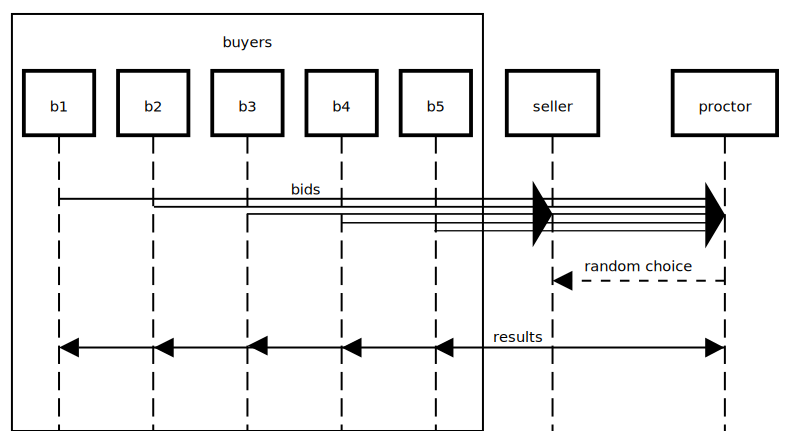
\includegraphics[width=13.5cm]{exercise.pdf}
  \end{minipage}
  \end{tabular}
  \caption{sequence diagram}
  \label{fig:usability-exercise-diagram}
    %%\Description{In the top section, twenty four lines of Haskell code using the MultiChor library, with a UML sequence diagram of that program.
%%	  }
  \end{mdframed}
\end{figure}


\end{document}
